\ifx\master\undefined% AUTOCOMPILE
% Allows for individual chapters to be compiled.

% Usage:
% \ifx\master\undefined% AUTOCOMPILE
% Allows for individual chapters to be compiled.

% Usage:
% \ifx\master\undefined% AUTOCOMPILE
% Allows for individual chapters to be compiled.

% Usage:
% \ifx\master\undefined\input{../settings/autocompile}\fi
% (place at start and end of chapter file)

\ifx\noprelim\undefined
    % first time included
    % input preamble files
    \input{../settings/phdsetup}

    \begin{document}
    \def\noprelim{}
\else
    % already included once
    % input post files

    \singlespacing
    \bibliographystyle{../bibliography/expanded}
    \bibliography{../bibliography/references}

    \end{document}
\fi\fi
% (place at start and end of chapter file)

\ifx\noprelim\undefined
    % first time included
    % input preamble files
    % [ USER VARIABLES ]

\def\PHDTITLE {Extensions of the Theory of Computational Mechanics}
\def\PHDAUTHOR{Evan Klose Friis}
\def\PHDSCHOOL{University of California, Davis}

\def\PHDMONTH {June}
\def\PHDYEAR  {2011}
\def\PHDDEPT {Physics}

\def\BSSCHOOL {University of California at San Diego}
\def\BSYEAR   {2005}

\def\PHDCOMMITTEEA{Professor John Conway}
\def\PHDCOMMITTEEB{Professor Robin Erbacher}
\def\PHDCOMMITTEEC{Professor Mani Tripathi}

% [ GLOBAL SETUP ]

\documentclass[letterpaper,oneside,11pt]{report}

\usepackage{calc}
\usepackage{breakcites}
\usepackage[newcommands]{ragged2e}

\usepackage[pdftex]{graphicx}
\usepackage{epstopdf}

%\usepackage{tikz}
%\usetikzlibrary{positioning} % [right=of ...]
%\usetikzlibrary{fit} % [fit= ...]

%\pgfdeclarelayer{background layer}
%\pgfdeclarelayer{foreground layer}
%\pgfsetlayers{background layer,main,foreground layer}

%\newenvironment{wrap}{\noindent\begin{minipage}[t]{\linewidth}\vspace{-0.5\normalbaselineskip}\centering}{\vspace{0.5\normalbaselineskip}\end{minipage}}

%% [Venn diagram environment]
%\newenvironment{venn2}
%{\begin{tikzpicture} [every pin/.style={text=black, text opacity=1.0, pin distance=0.5cm, pin edge={black!60, semithick}},
%% define a new style 'venn'
%venn/.style={circle, draw=black!60, semithick, minimum size = 4cm}]
%
%% create circle and give it external (pin) label
%\node[venn] (X) at (-1,0) [pin={150:$H[X]$}] {};
%\node[venn] (Y) at (1,0) [pin={30:$H[Y]$}] {};
%
%% place labels of the atoms by hand
%\node at (-1.9,0) {$H[X|Y]$};
%\node at (1.9,0) {$H[Y|X]$};
%\node at (0,0) {$I[X;Y]$};}
%{\end{tikzpicture}}

%\newcommand{\wrapmath}[1]{\begin{wrap}\begin{tikzpicture}[every node/.style={inner ysep=0ex, inner xsep=0em}]\node[] {$\displaystyle\begin{aligned} #1\end{aligned}$};\end{tikzpicture}\end{wrap}}

\renewenvironment{abstract}{\chapter*{Abstract}}{}
\renewcommand{\bibname}{Bibliography}
\renewcommand{\contentsname}{Table of Contents}

\makeatletter
\renewcommand{\@biblabel}[1]{\textsc{#1}}
\makeatother

% [ FONT SETTINGS ]

\usepackage[tbtags, intlimits, namelimits]{amsmath}
\usepackage[adobe-utopia]{mathdesign}

\DeclareSymbolFont{pazomath}{OMS}{zplm}{m}{n}
\DeclareSymbolFontAlphabet{\mathcal}{pazomath}
\SetMathAlphabet\mathcal{bold}{OMS}{zplm}{b}{n}

\SetSymbolFont{largesymbols}{normal}{OMX}{zplm}{m}{n}
\SetSymbolFont{largesymbols}{bold}{OMX}{zplm}{m}{n}
\SetSymbolFont{symbols}{normal}{OMS}{zplm}{m}{n}
\SetSymbolFont{symbols}{bold}{OMS}{zplm}{b}{n}

\renewcommand{\sfdefault}{phv}
\renewcommand{\ttdefault}{fvm}

\widowpenalty 8000
\clubpenalty  8000

% [ PAGE LAYOUT ]
\usepackage{geometry}
\geometry{lmargin = 1.5in}
\geometry{rmargin = 1.0in}
\geometry{tmargin = 1.0in}
\geometry{bmargin = 1.0in}

% [ PDF SETTINGS ]

\usepackage[final]{hyperref}
\hypersetup{breaklinks  = true}
\hypersetup{colorlinks  = true}
\hypersetup{linktocpage = false}
\hypersetup{linkcolor   = blue}
\hypersetup{citecolor   = green}
\hypersetup{urlcolor    = black}
\hypersetup{plainpages  = false}
\hypersetup{pageanchor  = true}
\hypersetup{pdfauthor   = {\PHDAUTHOR}}
\hypersetup{pdftitle    = {\PHDTITLE}}
\hypersetup{pdfsubject  = {Dissertation, \PHDSCHOOL}}
\urlstyle{same}

% [ LETTER SPACING ]

\usepackage[final]{microtype}
\microtypesetup{protrusion=compatibility}
\microtypesetup{expansion=false}

\newcommand{\upper}[1]{\MakeUppercase{#1}}
\let\lsscshape\scshape

\ifcase\pdfoutput\else\microtypesetup{letterspace=15}
\renewcommand{\scshape}{\lsscshape\lsstyle}
\renewcommand{\upper}[1]{\textls[50]{\MakeUppercase{#1}}}\fi

% [ LINE SPACING ]

\usepackage[doublespacing]{setspace}
\renewcommand{\displayskipstretch}{0.0}

\setlength{\parskip   }{0em}
\setlength{\parindent }{2em}

% [ TABLE FORMATTING ]

\usepackage{booktabs}
\setlength{\heavyrulewidth}{1.5\arrayrulewidth}
\setlength{\lightrulewidth}{1.0\arrayrulewidth}
\setlength{\doublerulesep }{2.0\arrayrulewidth}

% [ SECTION FORMATTING ]

\usepackage[largestsep,nobottomtitles*]{titlesec}
\renewcommand{\bottomtitlespace}{0.75in}

\titleformat{\chapter}[display]{\bfseries\huge\singlespacing}{\filleft\textsc{\LARGE \chaptertitlename\ \thechapter}}{-0.2ex}{\titlerule[3pt]\vspace{0.2ex}}[]

\titleformat{\section}{\LARGE}{\S\thesection\hspace{0.5em}}{0ex}{}
\titleformat{\subsection}{\Large}{\S\thesubsection\hspace{0.5em}}{0ex}{}
\titleformat{\subsubsection}{\large}{\thesubsubsection\hspace{0.5em}}{0ex}{}

\titlespacing*{\chapter}{0em}{6ex}{4ex plus 2ex minus 0ex}
\titlespacing*{\section}{0em}{2ex plus 3ex minus 1ex}{0.5ex plus 0.5ex minus 0.5ex}
\titlespacing*{\subsection}{0ex}{2ex plus 3ex minus 1ex}{0ex}
\titlespacing*{\subsubsection}{0ex}{2ex plus 0ex minus 1ex}{0ex}

% [ HEADER SETTINGS ]

\usepackage{fancyhdr}

\setlength{\headheight}{\normalbaselineskip}
\setlength{\footskip  }{0.5in}
\setlength{\headsep   }{0.5in-\headheight}

\fancyheadoffset[R]{0.5in}
\renewcommand{\headrulewidth}{0pt}
\renewcommand{\footrulewidth}{0pt}

\newcommand{\pagebox}{\parbox[r][\headheight][t]{0.5in}{\hspace\fill\thepage}}

\newcommand{\prelimheaders}{\ifx\prelim\undefined\renewcommand{\thepage}{\textit{\roman{page}}}\fancypagestyle{plain}{\fancyhf{}\fancyfoot[L]{\makebox[\textwidth-0.5in]{\thepage}}}\pagestyle{plain}\def\prelim{}\fi}

\newcommand{\normalheaders}{\renewcommand{\thepage}{\arabic{page}}\fancypagestyle{plain}{\fancyhf{}\fancyhead[R]{\pagebox}}\pagestyle{plain}}

\normalheaders{}

% [ CUSTOM COMMANDS ]

\newcommand{\signaturebox}[1]{\multicolumn{1}{p{4in}}{\vspace{3ex}}\\\midrule #1\\}

%\input{../includes/cmechabbrev}

% [some math stuff - maybe stick in sep file]
\usepackage{amsthm}
\usepackage{amscd}
\theoremstyle{plain}    \newtheorem{Lem}{Lemma}
\theoremstyle{plain}    \newtheorem*{ProLem}{Proof}
\theoremstyle{plain} 	\newtheorem{Cor}{Corollary}
\theoremstyle{plain} 	\newtheorem*{ProCor}{Proof}
\theoremstyle{plain} 	\newtheorem{The}{Theorem}
\theoremstyle{plain} 	\newtheorem*{ProThe}{Proof}
\theoremstyle{plain} 	\newtheorem{Prop}{Proposition}
\theoremstyle{plain} 	\newtheorem*{ProProp}{Proof}
\theoremstyle{plain} 	\newtheorem*{Conj}{Conjecture}
\theoremstyle{plain}	\newtheorem*{Rem}{Remark}
\theoremstyle{plain}	\newtheorem*{Def}{Definition} 
\theoremstyle{plain}	\newtheorem*{Not}{Notation}

% [uniform figure scaling - maybe this is not a good idea]
\def\figscale{.7}
\def\lscale{1.0}

% [FIX ME! - red makes it easier to spot]
\newcommand{\FIX}[1]{\textbf{\textcolor{red}{#1}}}


    \begin{document}
    \def\noprelim{}
\else
    % already included once
    % input post files

    \singlespacing
    \bibliographystyle{../bibliography/expanded}
    \bibliography{../bibliography/references}

    \end{document}
\fi\fi
% (place at start and end of chapter file)

\ifx\noprelim\undefined
    % first time included
    % input preamble files
    % [ USER VARIABLES ]

\def\PHDTITLE {Extensions of the Theory of Computational Mechanics}
\def\PHDAUTHOR{Evan Klose Friis}
\def\PHDSCHOOL{University of California, Davis}

\def\PHDMONTH {June}
\def\PHDYEAR  {2011}
\def\PHDDEPT {Physics}

\def\BSSCHOOL {University of California at San Diego}
\def\BSYEAR   {2005}

\def\PHDCOMMITTEEA{Professor John Conway}
\def\PHDCOMMITTEEB{Professor Robin Erbacher}
\def\PHDCOMMITTEEC{Professor Mani Tripathi}

% [ GLOBAL SETUP ]

\documentclass[letterpaper,oneside,11pt]{report}

\usepackage{calc}
\usepackage{breakcites}
\usepackage[newcommands]{ragged2e}

\usepackage[pdftex]{graphicx}
\usepackage{epstopdf}

%\usepackage{tikz}
%\usetikzlibrary{positioning} % [right=of ...]
%\usetikzlibrary{fit} % [fit= ...]

%\pgfdeclarelayer{background layer}
%\pgfdeclarelayer{foreground layer}
%\pgfsetlayers{background layer,main,foreground layer}

%\newenvironment{wrap}{\noindent\begin{minipage}[t]{\linewidth}\vspace{-0.5\normalbaselineskip}\centering}{\vspace{0.5\normalbaselineskip}\end{minipage}}

%% [Venn diagram environment]
%\newenvironment{venn2}
%{\begin{tikzpicture} [every pin/.style={text=black, text opacity=1.0, pin distance=0.5cm, pin edge={black!60, semithick}},
%% define a new style 'venn'
%venn/.style={circle, draw=black!60, semithick, minimum size = 4cm}]
%
%% create circle and give it external (pin) label
%\node[venn] (X) at (-1,0) [pin={150:$H[X]$}] {};
%\node[venn] (Y) at (1,0) [pin={30:$H[Y]$}] {};
%
%% place labels of the atoms by hand
%\node at (-1.9,0) {$H[X|Y]$};
%\node at (1.9,0) {$H[Y|X]$};
%\node at (0,0) {$I[X;Y]$};}
%{\end{tikzpicture}}

%\newcommand{\wrapmath}[1]{\begin{wrap}\begin{tikzpicture}[every node/.style={inner ysep=0ex, inner xsep=0em}]\node[] {$\displaystyle\begin{aligned} #1\end{aligned}$};\end{tikzpicture}\end{wrap}}

\renewenvironment{abstract}{\chapter*{Abstract}}{}
\renewcommand{\bibname}{Bibliography}
\renewcommand{\contentsname}{Table of Contents}

\makeatletter
\renewcommand{\@biblabel}[1]{\textsc{#1}}
\makeatother

% [ FONT SETTINGS ]

\usepackage[tbtags, intlimits, namelimits]{amsmath}
\usepackage[adobe-utopia]{mathdesign}

\DeclareSymbolFont{pazomath}{OMS}{zplm}{m}{n}
\DeclareSymbolFontAlphabet{\mathcal}{pazomath}
\SetMathAlphabet\mathcal{bold}{OMS}{zplm}{b}{n}

\SetSymbolFont{largesymbols}{normal}{OMX}{zplm}{m}{n}
\SetSymbolFont{largesymbols}{bold}{OMX}{zplm}{m}{n}
\SetSymbolFont{symbols}{normal}{OMS}{zplm}{m}{n}
\SetSymbolFont{symbols}{bold}{OMS}{zplm}{b}{n}

\renewcommand{\sfdefault}{phv}
\renewcommand{\ttdefault}{fvm}

\widowpenalty 8000
\clubpenalty  8000

% [ PAGE LAYOUT ]
\usepackage{geometry}
\geometry{lmargin = 1.5in}
\geometry{rmargin = 1.0in}
\geometry{tmargin = 1.0in}
\geometry{bmargin = 1.0in}

% [ PDF SETTINGS ]

\usepackage[final]{hyperref}
\hypersetup{breaklinks  = true}
\hypersetup{colorlinks  = true}
\hypersetup{linktocpage = false}
\hypersetup{linkcolor   = blue}
\hypersetup{citecolor   = green}
\hypersetup{urlcolor    = black}
\hypersetup{plainpages  = false}
\hypersetup{pageanchor  = true}
\hypersetup{pdfauthor   = {\PHDAUTHOR}}
\hypersetup{pdftitle    = {\PHDTITLE}}
\hypersetup{pdfsubject  = {Dissertation, \PHDSCHOOL}}
\urlstyle{same}

% [ LETTER SPACING ]

\usepackage[final]{microtype}
\microtypesetup{protrusion=compatibility}
\microtypesetup{expansion=false}

\newcommand{\upper}[1]{\MakeUppercase{#1}}
\let\lsscshape\scshape

\ifcase\pdfoutput\else\microtypesetup{letterspace=15}
\renewcommand{\scshape}{\lsscshape\lsstyle}
\renewcommand{\upper}[1]{\textls[50]{\MakeUppercase{#1}}}\fi

% [ LINE SPACING ]

\usepackage[doublespacing]{setspace}
\renewcommand{\displayskipstretch}{0.0}

\setlength{\parskip   }{0em}
\setlength{\parindent }{2em}

% [ TABLE FORMATTING ]

\usepackage{booktabs}
\setlength{\heavyrulewidth}{1.5\arrayrulewidth}
\setlength{\lightrulewidth}{1.0\arrayrulewidth}
\setlength{\doublerulesep }{2.0\arrayrulewidth}

% [ SECTION FORMATTING ]

\usepackage[largestsep,nobottomtitles*]{titlesec}
\renewcommand{\bottomtitlespace}{0.75in}

\titleformat{\chapter}[display]{\bfseries\huge\singlespacing}{\filleft\textsc{\LARGE \chaptertitlename\ \thechapter}}{-0.2ex}{\titlerule[3pt]\vspace{0.2ex}}[]

\titleformat{\section}{\LARGE}{\S\thesection\hspace{0.5em}}{0ex}{}
\titleformat{\subsection}{\Large}{\S\thesubsection\hspace{0.5em}}{0ex}{}
\titleformat{\subsubsection}{\large}{\thesubsubsection\hspace{0.5em}}{0ex}{}

\titlespacing*{\chapter}{0em}{6ex}{4ex plus 2ex minus 0ex}
\titlespacing*{\section}{0em}{2ex plus 3ex minus 1ex}{0.5ex plus 0.5ex minus 0.5ex}
\titlespacing*{\subsection}{0ex}{2ex plus 3ex minus 1ex}{0ex}
\titlespacing*{\subsubsection}{0ex}{2ex plus 0ex minus 1ex}{0ex}

% [ HEADER SETTINGS ]

\usepackage{fancyhdr}

\setlength{\headheight}{\normalbaselineskip}
\setlength{\footskip  }{0.5in}
\setlength{\headsep   }{0.5in-\headheight}

\fancyheadoffset[R]{0.5in}
\renewcommand{\headrulewidth}{0pt}
\renewcommand{\footrulewidth}{0pt}

\newcommand{\pagebox}{\parbox[r][\headheight][t]{0.5in}{\hspace\fill\thepage}}

\newcommand{\prelimheaders}{\ifx\prelim\undefined\renewcommand{\thepage}{\textit{\roman{page}}}\fancypagestyle{plain}{\fancyhf{}\fancyfoot[L]{\makebox[\textwidth-0.5in]{\thepage}}}\pagestyle{plain}\def\prelim{}\fi}

\newcommand{\normalheaders}{\renewcommand{\thepage}{\arabic{page}}\fancypagestyle{plain}{\fancyhf{}\fancyhead[R]{\pagebox}}\pagestyle{plain}}

\normalheaders{}

% [ CUSTOM COMMANDS ]

\newcommand{\signaturebox}[1]{\multicolumn{1}{p{4in}}{\vspace{3ex}}\\\midrule #1\\}

%%%% macros fro standard references
%\eqref provided by amsmath
\newcommand{\figref}[1]{Fig.~\ref{#1}}
\newcommand{\tableref}[1]{Table~\ref{#1}}
\newcommand{\refcite}[1]{Ref.~\cite{#1}}

% Abbreviations from CMPPSS:

\newcommand{\eM}     {\mbox{$\epsilon$-machine}}
\newcommand{\eMs}    {\mbox{$\epsilon$-machines}}
\newcommand{\EM}     {\mbox{$\epsilon$-Machine}}
\newcommand{\EMs}    {\mbox{$\epsilon$-Machines}}
\newcommand{\eT}     {\mbox{$\epsilon$-transducer}}
\newcommand{\eTs}    {\mbox{$\epsilon$-transducers}}
\newcommand{\ET}     {\mbox{$\epsilon$-Transducer}}
\newcommand{\ETs}    {\mbox{$\epsilon$-Transducers}}

% Processes and sequences

\newcommand{\Process}{\mathcal{P}}

\newcommand{\ProbMach}{\Prob_{\mathrm{M}}}
\newcommand{\Lmax}   { {L_{\mathrm{max}}}}
\newcommand{\MeasAlphabet}	{\mathcal{A}}
% Original
%\newcommand{\MeasSymbol}   { {S} }
%\newcommand{\meassymbol}   { {s} }
% New symbol
\newcommand{\MeasSymbol}   { {X} }
\newcommand{\meassymbol}   { {x} }
\newcommand{\BiInfinity}	{ \overleftrightarrow {\MeasSymbol} }
\newcommand{\biinfinity}	{ \overleftrightarrow {\meassymbol} }
\newcommand{\Past}	{ \overleftarrow {\MeasSymbol} }
\newcommand{\past}	{ {\overleftarrow {\meassymbol}} }
\newcommand{\pastprime}	{ {\past}^{\prime}}
\newcommand{\Future}	{ \overrightarrow{\MeasSymbol} }
\newcommand{\future}	{ \overrightarrow{\meassymbol} }
\newcommand{\futureprime}	{ {\future}^{\prime}}
\newcommand{\PastPrime}	{ {\Past}^{\prime}}
\newcommand{\FuturePrime}	{ {\overrightarrow{\meassymbol}}^\prime }
\newcommand{\PastDblPrime}	{ {\overleftarrow{\meassymbol}}^{\prime\prime} }
\newcommand{\FutureDblPrime}	{ {\overrightarrow{\meassymbol}}^{\prime\prime} }
\newcommand{\pastL}	{ {\overleftarrow {\meassymbol}}{}^L }
\newcommand{\PastL}	{ {\overleftarrow {\MeasSymbol}}{}^L }
\newcommand{\PastLt}	{ {\overleftarrow {\MeasSymbol}}_t^L }
\newcommand{\PastLLessOne}	{ {\overleftarrow {\MeasSymbol}}^{L-1} }
\newcommand{\futureL}	{ {\overrightarrow{\meassymbol}}{}^L }
\newcommand{\FutureL}	{ {\overrightarrow{\MeasSymbol}}{}^L }
\newcommand{\FutureLt}	{ {\overrightarrow{\MeasSymbol}}_t^L }
\newcommand{\FutureLLessOne}	{ {\overrightarrow{\MeasSymbol}}^{L-1} }
\newcommand{\pastLprime}	{ {\overleftarrow {\meassymbol}}^{L^\prime} }
\newcommand{\futureLprime}	{ {\overrightarrow{\meassymbol}}^{L^\prime} }
\newcommand{\AllPasts}	{ { \overleftarrow {\rm {\bf \MeasSymbol}} } }
\newcommand{\AllFutures}	{ \overrightarrow {\rm {\bf \MeasSymbol}} }
\newcommand{\FutureSet}	{ \overrightarrow{\bf \MeasSymbol}}

% Causal states and epsilon-machines
\newcommand{\CausalState}	{ \mathcal{S} }
\newcommand{\CausalStatePrime}	{ {\CausalState}^{\prime}}
\newcommand{\causalstate}	{ \sigma }
\newcommand{\CausalStateSet}	{ \boldsymbol{\CausalState} }
\newcommand{\AlternateState}	{ \mathcal{R} }
\newcommand{\AlternateStatePrime}	{ {\cal R}^{\prime} }
\newcommand{\alternatestate}	{ \rho }
\newcommand{\alternatestateprime}	{ {\rho^{\prime}} }
\newcommand{\AlternateStateSet}	{ \boldsymbol{\AlternateState} }
\newcommand{\PrescientState}	{ \widehat{\AlternateState} }
\newcommand{\prescientstate}	{ \widehat{\alternatestate} }
\newcommand{\PrescientStateSet}	{ \boldsymbol{\PrescientState}}
\newcommand{\CausalEquivalence}	{ {\sim}_{\epsilon} }
\newcommand{\CausalEquivalenceNot}	{ {\not \sim}_{\epsilon}}

\newcommand{\NonCausalEquivalence}	{ {\sim}_{\eta} }
\newcommand{\NextObservable}	{ {\overrightarrow {\MeasSymbol}}^1 }
\newcommand{\LastObservable}	{ {\overleftarrow {\MeasSymbol}}^1 }
%\newcommand{\Prob}		{ {\rm P}}
\newcommand{\Prob}      {\Pr} % use standard command
\newcommand{\ProbAnd}	{ {,\;} }
\newcommand{\LLimit}	{ {L \rightarrow \infty}}
\newcommand{\Cmu}		{C_\mu}
\newcommand{\hmu}		{h_\mu}
\newcommand{\EE}		{{\bf E}}
\newcommand{\Measurable}{{\bf \mu}}

% Process Crypticity
\newcommand{\PC}		{\chi}
\newcommand{\FuturePC}		{\PC^+}
\newcommand{\PastPC}		{\PC^-}
% Causal Irreversibility
\newcommand{\CI}		{\Xi}
\newcommand{\ReverseMap}	{r}
\newcommand{\ForwardMap}	{f}

% Abbreviations from IB:
% None that aren't already in CMPPSS

% Abbreviations from Extensive Estimation:
\newcommand{\EstCausalState}	{\widehat{\CausalState}}
\newcommand{\estcausalstate}	{\widehat{\causalstate}}
\newcommand{\EstCausalStateSet}	{\boldsymbol{\EstCausalState}}
\newcommand{\EstCausalFunc}	{\widehat{\epsilon}}
\newcommand{\EstCmu}		{\widehat{\Cmu}}
\newcommand{\PastLOne}	{{\Past}^{L+1}}
\newcommand{\pastLOne}	{{\past}^{L+1}}

% Abbreviations from $\epsilon$-Transducers:
\newcommand{\InAlphabet}	{ \mathcal{A}}
\newcommand{\insymbol}		{ a}
\newcommand{\OutAlphabet}	{ \mathcal{B}}
\newcommand{\outsymbol}		{ b}
\newcommand{\InputSimple}	{ X}
\newcommand{\inputsimple}	{ x}
\newcommand{\BottleneckVar}	{\tilde{\InputSimple}}
\newcommand{\bottleneckvar}	{\tilde{\inputsimple}}
\newcommand{\InputSpace}	{ \mathbf{\InputSimple}}
\newcommand{\InputBi}	{ \overleftrightarrow {\InputSimple} }
\newcommand{\inputbi}	{ \overleftrightarrow {\inputsimple} }
\newcommand{\InputPast}	{ \overleftarrow {\InputSimple} }
\newcommand{\inputpast}	{ \overleftarrow {\inputsimple} }
\newcommand{\InputFuture}	{ \overrightarrow {\InputSimple} }
\newcommand{\inputfuture}	{ \overrightarrow {\inputsimple} }
\newcommand{\NextInput}	{ {{\InputFuture}^{1}}}
\newcommand{\NextOutput}	{ {\OutputFuture}^{1}}
\newcommand{\OutputSimple}	{ Y}
\newcommand{\outputsimple}	{ y}
\newcommand{\OutputSpace}	{ \mathbf{\OutputSimple}}
\newcommand{\OutputBi}	{ \overleftrightarrow{\OutputSimple} }
\newcommand{\outputbi}	{ \overleftrightarrow{\outputsimple} }
\newcommand{\OutputPast}	{ \overleftarrow{\OutputSimple} }
\newcommand{\outputpast}	{ \overleftarrow{\outputsimple} }
\newcommand{\OutputFuture}	{ \overrightarrow{\OutputSimple} }
\newcommand{\outputfuture}	{ \overrightarrow{\outputsimple} }
\newcommand{\OutputL}	{ {\OutputFuture}^L}
\newcommand{\outputL}	{ {\outputfuture}^L}
\newcommand{\InputLLessOne}	{ {\InputFuture}^{L-1}}
\newcommand{\inputLlessone}	{ {\inputufutre}^{L-1}}
\newcommand{\OutputPastLLessOne}	{{\OutputPast}^{L-1}_{-1}}
\newcommand{\outputpastLlessone}	{{\outputpast}^{L-1}}
\newcommand{\OutputPastLessOne}	{{\OutputPast}_{-1}}
\newcommand{\outputpastlessone}	{{\outputpast}_{-1}}
\newcommand{\OutputPastL}	{{\OutputPast}^{L}}
\newcommand{\OutputLPlusOne}	{ {\OutputFuture}^{L+1}}
\newcommand{\outputLplusone}	{ {\outputfutre}^{L+1}}
\newcommand{\InputPastL}	{{\InputPast}^{L}}
\newcommand{\inputpastL}	{{\inputpast}^{L}}
\newcommand{\JointPast}	{{(\InputPast,\OutputPast)}}
\newcommand{\jointpast}	{{(\inputpast,\outputpast)}}
\newcommand{\jointpastone}	{{(\inputpast_1,\outputpast_1)}}
\newcommand{\jointpasttwo}	{{(\inputpast_2,\outputpast_2)}}
\newcommand{\jointpastprime} {{({\inputpast}^{\prime},{\outputpast}^{\prime})}}
\newcommand{\NextJoint}	{{(\NextInput,\NextOutput)}}
\newcommand{\nextjoint}	{{(\insymbol,\outsymbol)}}
\newcommand{\AllInputPasts}	{ { \overleftarrow {\rm \InputSpace}}}
\newcommand{\AllOutputPasts}	{ {\overleftarrow {\rm \OutputSpace}}}
\newcommand{\DetCausalState}	{ {{\cal S}_D }}
\newcommand{\detcausalstate}	{ {{\sigma}_D} }
\newcommand{\DetCausalStateSet}	{ \boldsymbol{{\CausalState}_D}}
\newcommand{\DetCausalEquivalence}	{ {\sim}_{{\epsilon}_{D}}}
\newcommand{\PrescientEquivalence}	{ {\sim}_{\widehat{\eta}}}
\newcommand{\FeedbackCausalState}	{ \mathcal{F}}
\newcommand{\feedbackcausalstate}	{ \phi}
\newcommand{\FeedbackCausalStateSet}	{ \mathbf{\FeedbackCausalState}}
\newcommand{\JointCausalState}		{ \mathcal{J}}
\newcommand{\JointCausalStateSet}	{ \mathbf{\JointCausalState}}
\newcommand{\UtilityFunctional}	{ {\mathcal{L}}}
\newcommand{\NatureState}	{ {\Omega}}
\newcommand{\naturestate}	{ {\omega}}
\newcommand{\NatureStateSpace}	{ {\mathbf{\NatureState}}}
\newcommand{\AnAction}	{ {A}}
\newcommand{\anaction}	{ {a}}
\newcommand{\ActionSpace}	{ {\mathbf{\AnAction}}}

% Abbreviations from RURO:
\newcommand{\InfoGain}[2] { \mathcal{D} \left( {#1} || {#2} \right) }

% Abbreviations from Upper Bound:
\newcommand{\lcm}	{{\rm lcm}}
% Double-check that this isn't in the math set already!

% Abbreviations from Emergence in Space
\newcommand{\ProcessAlphabet}	{\MeasAlphabet}
\newcommand{\ProbEst}			{ {\widehat{\Prob}_N}}
\newcommand{\STRegion}			{ {\mathrm K}}
\newcommand{\STRegionVariable}		{ K}
\newcommand{\stregionvariable}		{ k}
\newcommand{\GlobalPast}		{ \overleftarrow{G}} 
\newcommand{\globalpast}		{ \overleftarrow{g}} 
\newcommand{\GlobalFuture}		{ \overrightarrow{G}}
\newcommand{\globalfuture}		{ \overrightarrow{g}}
\newcommand{\GlobalState}		{ \mathcal{G}}
\newcommand{\globalstate}		{ \gamma}
\newcommand{\GlobalStateSet}		{ {\mathbf \GlobalState}}
\newcommand{\LocalPast}			{ \overleftarrow{L}} 
\newcommand{\localpast}			{ \overleftarrow{l}}
\newcommand{\AllLocalPasts}		{ \mathbf{\LocalPast}}
\newcommand{\LocalPastRegion}		{ \overleftarrow{\mathrm L}}
\newcommand{\LocalFuture}		{ \overrightarrow{L}}
\newcommand{\localfuture}		{ \overrightarrow{l}}
\newcommand{\LocalFutureRegion}		{ \overrightarrow{\mathrm L}}
\newcommand{\LocalState}		{ \mathcal{L}}
\newcommand{\localstate}		{ \lambda}
\newcommand{\LocalStateSet}		{ {\mathbf \LocalState}}
\newcommand{\PatchPast}			{ \overleftarrow{P}}
\newcommand{\patchpast}			{ \overleftarrow{p}}
\newcommand{\PatchPastRegion}		{ \overleftarrow{\mathrm P}}
\newcommand{\PatchFuture}		{ \overrightarrow{P}}
\newcommand{\patchfuture}		{ \overrightarrow{p}}
\newcommand{\PatchFutureRegion}		{ \overrightarrow{\mathrm P}}
\newcommand{\PatchState}		{ \mathcal{P}}
\newcommand{\patchstate}		{ \pi}
\newcommand{\PatchStateSet}		{ {\mathbf \PatchState}}
\newcommand{\LocalStatesInPatch}	{\vec{\LocalState}}
\newcommand{\localstatesinpatch}	{\vec{\localstate}}
\newcommand{\PointInstantX}		{ {\mathbf x}}
% Galles's original LaTeX for the cond. indep. symbol follows:
\newcommand{\compos}{\mbox{$~\underline{~\parallel~}~$}}
\newcommand{\ncompos}{\not\hspace{-.15in}\compos}
\newcommand{\indep}			{ \rotatebox{90}{$\models$}}
\newcommand{\nindep}	{\not\hspace{-.05in}\indep}
\newcommand{\LocalEE}	{{\EE}^{loc}}
\newcommand{\EEDensity}	{\overline{\LocalEE}}
\newcommand{\LocalCmu}	{{\Cmu}^{loc}}
\newcommand{\CmuDensity}	{\overline{\LocalCmu}}

%%%%%%%%%%% added by sasa
\newcommand{\FinPast}[1]	{ \overleftarrow {\MeasSymbol} \stackrel{{#1}}{}}
\newcommand{\finpast}[1]  	{ \overleftarrow {\meassymbol}  \stackrel{{#1}}{}}
\newcommand{\FinFuture}[1]		{ \overrightarrow{\MeasSymbol} \stackrel{{#1}}{}}
\newcommand{\finfuture}[1]		{ \overrightarrow{\meassymbol} \stackrel{{#1}}{}}

\newcommand{\Partition}	{ \AlternateState }
\newcommand{\partitionstate}	{ \alternatestate }
\newcommand{\PartitionSet}	{ \AlternateStateSet }
\newcommand{\Fdet}   { F_{\rm det} }

\newcommand{\Dkl}[2] { D_{\rm KL} \left( {#1} || {#2} \right) }

\newcommand{\Period}	{p}

% To take into account time direction
\newcommand{\forward}{+}
\newcommand{\reverse}{-}
%\newcommand{\forwardreverse}{\:\!\diamond} % \pm
\newcommand{\forwardreverse}{\pm} % \pm
\newcommand{\FutureProcess}	{ {\Process}^{\forward} }
\newcommand{\PastProcess}	{ {\Process}^{\reverse} }
\newcommand{\FutureCausalState}	{ {\CausalState}^{\forward} }
\newcommand{\futurecausalstate}	{ \sigma^{\forward} }
\newcommand{\altfuturecausalstate}	{ \sigma^{\forward\prime} }
\newcommand{\PastCausalState}	{ {\CausalState}^{\reverse} }
\newcommand{\pastcausalstate}	{ \sigma^{\reverse} }
\newcommand{\BiCausalState}		{ {\CausalState}^{\forwardreverse} }
\newcommand{\bicausalstate}		{ {\sigma}^{\forwardreverse} }
\newcommand{\FutureCausalStateSet}	{ {\CausalStateSet}^{\forward} }
\newcommand{\PastCausalStateSet}	{ {\CausalStateSet}^{\reverse} }
\newcommand{\BiCausalStateSet}	{ {\CausalStateSet}^{\forwardreverse} }
\newcommand{\eMachine}	{ M }
\newcommand{\FutureEM}	{ {\eMachine}^{\forward} }
\newcommand{\PastEM}	{ {\eMachine}^{\reverse} }
\newcommand{\BiEM}		{ {\eMachine}^{\forwardreverse} }
\newcommand{\BiEquiv}	{ {\sim}^{\forwardreverse} }
\newcommand{\Futurehmu}	{ h_\mu^{\forward} }
\newcommand{\Pasthmu}	{ h_\mu^{\reverse} }
\newcommand{\FutureCmu}	{ C_\mu^{\forward} }
\newcommand{\PastCmu}	{ C_\mu^{\reverse} }
\newcommand{\BiCmu}		{ C_\mu^{\forwardreverse} }
\newcommand{\FutureEps}	{ \epsilon^{\forward} }
\newcommand{\PastEps}	{ \epsilon^{\reverse} }
\newcommand{\BiEps}	{ \epsilon^{\forwardreverse} }
\newcommand{\FutureSim}	{ \sim^{\forward} }
\newcommand{\PastSim}	{ \sim^{\reverse} }
% Used arrows for awhile, more or less confusing?
%\newcommand{\FutureCausalState}	{ \overrightarrow{\CausalState} }
%\newcommand{\PastCausalState}	{ \overleftarrow{\CausalState} }
%\newcommand{\eMachine}	{ M }
%\newcommand{\FutureEM}	{ \overrightarrow{\eMachine} }
%\newcommand{\PastEM}	{ \overleftarrow{\eMachine} }
%\newcommand{\FutureCmu}	{ \overrightarrow{\Cmu} }
%\newcommand{\PastCmu}	{ \overleftarrow{\Cmu} }

%% time-reversing and mixed state presentation operators
\newcommand{\TR}{\mathcal{T}}
\newcommand{\MSP}{\mathcal{U}}
\newcommand{\one}{\mathbf{1}}

%% (cje)
%% Provide a command \ifpm which is true when \pm 
%% is meant to be understood as "+ or -". This is
%% different from the usage in TBA.
\newif\ifpm 
\edef\tempa{\forwardreverse}
\edef\tempb{\pm}
\ifx\tempa\tempb
   \pmfalse
\else
   \pmtrue  
\fi





% [some math stuff - maybe stick in sep file]
\usepackage{amsthm}
\usepackage{amscd}
\theoremstyle{plain}    \newtheorem{Lem}{Lemma}
\theoremstyle{plain}    \newtheorem*{ProLem}{Proof}
\theoremstyle{plain} 	\newtheorem{Cor}{Corollary}
\theoremstyle{plain} 	\newtheorem*{ProCor}{Proof}
\theoremstyle{plain} 	\newtheorem{The}{Theorem}
\theoremstyle{plain} 	\newtheorem*{ProThe}{Proof}
\theoremstyle{plain} 	\newtheorem{Prop}{Proposition}
\theoremstyle{plain} 	\newtheorem*{ProProp}{Proof}
\theoremstyle{plain} 	\newtheorem*{Conj}{Conjecture}
\theoremstyle{plain}	\newtheorem*{Rem}{Remark}
\theoremstyle{plain}	\newtheorem*{Def}{Definition} 
\theoremstyle{plain}	\newtheorem*{Not}{Notation}

% [uniform figure scaling - maybe this is not a good idea]
\def\figscale{.7}
\def\lscale{1.0}

% [FIX ME! - red makes it easier to spot]
\newcommand{\FIX}[1]{\textbf{\textcolor{red}{#1}}}


    \begin{document}
    \def\noprelim{}
\else
    % already included once
    % input post files

    \singlespacing
    \bibliographystyle{../bibliography/expanded}
    \bibliography{../bibliography/references}

    \end{document}
\fi\fi

\chapter{The Standard Model and Beyond}
\label{ch:theory}

\section{The Standard Model}
%
The standard model (SM) is a ``theory of almost everything'' that describes the
interactions of elementary particles.  The SM is a quantum
field theory, first appearing in its modern form in the middle of the 20th
century.  The model is the synthesis of the independent theories of
electromagnetism, and the weak and strong nuclear forces.  Each of these
theories was used to describe different phenomena, which each have extremely
different strengths and act at different scales.  The interaction of light and
matter is described by quantum electrodynamics~(QED), a relativistic field
extension of the theory of electromagnetism.  The physics of radioactivity and
nuclear decay was described by the Fermi theory of weak interactions and the
forces that strong nuclear force binds the nuclei of atoms was described by
Yukawa.  An overview of these theories will be presented in this chapter.  

The feature that united the disparate theories into the SM was the
application of the principle of local gauge invariance. The principle of
gauge invariance first found success in QED, which predicted electromagnetic
phenomenon with astounding accuracy.  Local gauge invariance is now believed to
a fundamental feature of nature that underpins all theories of elementary
particles.  Furthermore, the development of the complete SM as it is
known today was precipitated by Goldstones's work on spontaneous symmetry
breaking~\cite{Goldstone:1961eq,PhysRev.127.965}, which produces an effective
Lagrangian with additional massless ``Goldstone'' bosons.  Higgs (and
others)~\cite{PhysRevLett.13.321, PhysRevLett.13.508,PhysRevLett.13.585}
developed these ideas into what is ultimately called the ``Higgs mechanism,''
which uses a combination of new fields with broken symmetry to give mass to the
Goldstone bosons.

In the 1960s, Glashow~\cite{Glashow:1961tr}, Weinberg~\cite{Weinberg:1967tq}, 
and Salam~\cite{Salam:1968rm} developed the above ideas into the
electroweak model, which unified QED with the weak force using intermediate weak
bosons in a gauge theory with symmetry that is spontaneously broken using the Higgs
mechanism.  This unified theory has been incredibly experimentally successful
and is the foundation of modern particle theory.

\subsection{Quantum Electrodynamics and Gauge Invariance}
\label{sec:QEDandGaugeInvariance}
%
The theory of QED is a modern extension of Maxwell's theory of
electromagnetism, describing the interaction of matter with light.  The
development of QED is a result of efforts to develop a quantum mechanical
formulation of electromagnetism compatible with the theory of special relativity.
QED is a \emph{gauge} theory, which means that the physical observables are
invariant under local gauge transformations.  Requiring local gauge
invariance gives rise to a ``gauge'' field, which can be interpreted as 
particles that are exchanged during an interaction.  

In the following, we first describe the Dirac equation for a free electron,
which is the relativistic extension of the Schroedinger equation for spin~$1/2$
particles.  We then show that requiring the corresponding Lagrangian of the free
charged particle to be invariant under local gauge transformations creates an
effective gauge boson field.  This ``gauge field'' creates terms in the
Lagrangian that represent interactions between the particles.

% Dirac equation comes from pg. 215 of Griffiths
The Dirac equation is the equation of motion of a free spin~$1/2$ particle of
mass~$m$ and is derived from the energy--momentum relationship of relativity
\begin{equation}
  p^{\mu}p_\mu - m^2c^2 = 0.
  \label{eq:EnergyPRelationship}
\end{equation}
Dirac sought to express this relationship in the framework of quantum mechanics
by applying the transformation
\begin{equation}
  p_\mu \to i \hbar \partial_\mu 
  \label{eq:QuantizeMomentumTransformation}
\end{equation}
to equation Equation~\ref{eq:EnergyPRelationship}, but with the requirement that
the resulting equation be first order in time.\footnote{A detailed
discussion of this topic is available in~\cite{Griffiths:IntroParticle}.}
To achieve this, Dirac factorized Equation~\ref{eq:EnergyPRelationship} into 
\begin{equation}
  (\gamma^\kappa p_\kappa + mc)(\gamma^\mu p_\mu - mc) = 0,
  \label{eq:DiracEquationFactorized}
\end{equation}
where $\gamma^\mu$ is a set of four $4\times4$ matrices referred to as the Dirac
matrices.  The equation of motion is obtained by choosing either term (they are
equivalent) from the
left hand side of Equation~\ref{eq:DiracEquationFactorized} and
making the substitution in Equation~\ref{eq:QuantizeMomentumTransformation}.
\begin{equation}
  i \hbar \gamma^\mu \partial_\mu \psi - mc \psi = 0.
  \label{eq:DiracEquation}
\end{equation}
The solutions $\psi$ of the Dirac equation are called ``Dirac spinors,'' and
represent the quantum mechanical state of spin~$1/2$ particles.

The Lagrangian corresponding to the Dirac equation~(\ref{eq:DiracEquation}) is
\begin{equation}
  \mathcal{L} = \overline \psi (i\hbar c\gamma^\mu \partial_\mu - mc^2) \psi,
  \label{eq:FreeQEDLagrangian}
\end{equation}
where $\psi$ is the spinor field of the particle in question, $\hbar$ is Planck's
constant, $c$ the speed of light, and $\gamma^\mu$ are the Dirac matrices.  As
$\overline\psi$ is the Hermitian conjugate of $\psi$, the Lagrangian is invariant
under the global gauge transformation 
\begin{equation}
  \psi' \to e^{i\theta}\psi.
  \label{eq:U1GaugeTransform}
\end{equation}
The Lagrangian is invariant under \emph{local} gauge translations if $\theta$
can be defined differently at each point in space, \ie if $\theta = \theta(x)$
in Equation~\ref{eq:U1GaugeTransform}.  However, as the derivative operator
$\partial_\mu$ in Equation~\ref{eq:FreeQEDLagrangian} does not commute with
$\theta(x)$, the Lagrangian must be modified to satisfy local gauge invariance.
This modification is accomplished with the use of a ``gauge covariant
derivative.''  By making the replacement 
\begin{equation} 
  \partial_\mu \to D_\mu = \partial_\mu - \frac{ie}{\hbar}A^\mu      
  \nonumber
\end{equation}
in Equation~\ref{eq:FreeQEDLagrangian}, where 
$A^\mu = \partial^\mu \theta(x)$ and $e$ is the electric charge, the Lagrangian
becomes locally gauge invariant:
\begin{equation}
  \mathcal{L} = \overline \psi (i\hbar c\gamma^\mu D_\mu - mc^2) \psi.
  \label{eq:LocalQEDLagrangian}
\end{equation}
The difference between
the locally (\ref{eq:LocalQEDLagrangian}) and the globally 
(\ref{eq:FreeQEDLagrangian}) gauge invariant Lagrangian is then
\begin{equation}
  \mathcal{L}_{int} = \frac{e}{\hbar}\overline\psi\gamma^\mu\psi A_\mu.
  \nonumber
\end{equation}
This term can be interpreted as the coupling between the particle and the gauge
boson (force carrier) fields.  The coupling is proportional to the constant $e$,
which is associated with the electric charge.  This is consistent with the
experimental observation that particles with zero electric charge do not
interact electromagnetically with each other.  In this interpretation, the
electromagnetic force between two charged particles is caused by the exchange of
gauge bosons (photons).  The existence of this ``minimal coupling'' is
\emph{required} if the Lagrangian is to satisfy local gauge invariance. The
addition of a term with the gauge Field Strength Tensor to represent the kinetic
term of the gauge (photon) field yields the QED Lagrangian:
\begin{equation}
  \mathcal{L}_{QED} = \overline \psi (i\hbar c\gamma^\mu D_\mu - mc^2) \psi -
  \frac{1}{4\mu_0}F_{\mu\nu}F^{\mu\nu}.
  \nonumber
\end{equation}

The gauge symmetry group of QED is $U(1)$, the unitary group of degree 1.  This
symmetry can be visualized as a rotation of a two--dimensional unit vector. (The
application of the gauge transformation $e^{i\theta}$ rotates a number in the
complex plane.)  In a gauge theory the symmetry group of the gauge
transformation defines the behavior of the gauge bosons and thus the
interactions of the theory.  

\subsection{The Weak Interactions}
\label{sec:WeakInteractions}
The theory of Weak Interactions was created to describe the physics of
radioactive decay.  The first formulation of the theory was done by
Fermi~\cite{Fermi:1934hr} to explain the phenomenon of the $\beta$
decay of neutrons. The initial theory was a four-fermion ``contact'' theory.  In
a contact theory, all four fermions come involved in the $\beta$--decay are
connected at a single vertex.  The Fermi theory Hamiltonian for the
$\beta$--decay of a proton is then~\cite{Morii:SMandBSM}
\begin{equation}
  H = \frac{G_\beta}{\sqrt{2}}
  \left[\overline \psi_p \gamma_\mu (1 - g_A\gamma_5)\psi_n\right]
  \left[[\overline \psi_e \gamma^\mu (1 - \gamma_5) \psi_\nu\right] + h.c., 
 \label{eq:FermiTheoryHamiltonian}
\end{equation}
where $G_\beta$ is the Fermi constant and $g_A$ is the relative fraction of the
interaction with axially Lorentz structure.  The value of $g_A$ was determined
experimentally to be $1.26$.  One of the most notable things discovered about
the weak force is that weak interactions violate parity; that is, the physics of
the interaction change (or become disallowed) under inversion of the spatial
coordinates.  This is evidenced by the $(1-\gamma_5)$ term in
Equation~\ref{eq:FermiTheoryHamiltonian}.  This term is the ``helicity
operator''; the left and right ``handed'' helicity states are eigenstates states
of this term.
\begin{eqnarray}
  h = (1 - \gamma_5)/2 \nonumber \\
  h\psi_R = \frac{1}{2}\psi_R \nonumber \\ 
  h\psi_L = -\frac{1}{2}\psi_L \nonumber
\end{eqnarray}
It is observed that only left--chiral neutrinos (or right--chiral
anti--neutrinos) participate in the weak interaction.

The Fermi interaction can describe both nuclear $\beta$ decay ($p \to n + e^+ +
\overline{\nu}_e$) as well as the decay of a muon into an electron ($\mu \to
\nu_\mu + e + \overline{\nu}_e$, Figure~\ref{fig:MuonDecayContact}).
Furthermore, the coupling constant $G$ is found to be a \emph{universal}
constant in weak interactions, in that it is the same for interactions
regardless of the particle species participating in the interaction.  That is,
$G_\mu = G_e = G_F$.  Using an Hamiltonian analogous to
Equation~\ref{eq:FermiTheoryHamiltonian} for muon decay, the decay amplitude $M$
is found to be
\begin{equation}
  M = \frac{G_F}{\sqrt{2}}
  \left[\overline u_{\nu_\mu} \gamma_\rho \frac{1 - \gamma_5}{2} u_\mu\right]  
  \left[\overline u_{\nu_e} \gamma_\rho \frac{1 - \gamma_5}{2} u_e\right].
  \label{eq:ContactAmplitudeMuonDecay}
\end{equation}

However, the contact interaction form of
Fermi's theory is not complete.  When applied to scattering processes, the
interaction violates unitarity: the calculated cross section grows with the
center of mass energy, so that for some energy the probability for an
interaction is greater than one.  Furthermore, the techniques successfully used
to ``renormalize''\footnote{Renormalization of quantum field theories is a broad
topic beyond the scope of this thesis.  Briefly, the process involves
``absorbing'' infinite divergences that occur in higher--order interactions into
physical observables~\cite{Griffiths:IntroParticle}.} QED fail when applied to
the Fermi interaction.
\begin{figure}
  \centering
  \begin{fmffile}{muon_decay}
    \begin{fmfgraph*}(120,75)
    \fmfleft{i1}
    \fmfright{o1,o2,o3}
    %\fmftop{i2,d2,o2}
    \fmf{fermion}{i1,v1,o1}
    \fmf{fermion}{v1,o2}
    \fmf{fermion}{o3,v1}
    \fmflabel{$\mu^-$}{i1}
    \fmflabel{$\nu_\mu$}{o1}
    \fmflabel{$\overline \nu_e$}{o3}
    \fmflabel{$e^-$}{o2}
    \fmflabel{$G_F$}{v1}
    \end{fmfgraph*}
  \end{fmffile}
  \caption[Fermi contact interaction diagram]{Feynamn diagram of muon decay
  in Fermi contact interaction theory.}
  \label{fig:MuonDecayContact}
\end{figure}
\begin{figure}
  \centering
  \begin{fmffile}{muon_decay_propagator}
    \begin{fmfgraph*}(120,75)
    \fmfleft{i1}
    \fmfright{o1,o2,o3}
    %\fmftop{i2,d2,o2}
    \fmf{fermion}{i1,v1,o1}
    \fmf{photon, label=$W^-$}{v1,v2}
    \fmf{fermion}{v2,o2}
    \fmf{fermion}{v2,o3}
    \fmflabel{$\mu^-$}{i1}
    \fmflabel{$\nu_\mu$}{o1}
    \fmflabel{$\overline \nu_e$}{o3}
    \fmflabel{$e^-$}{o2}
    \end{fmfgraph*}
  \end{fmffile}
  \caption[Muon decaying through intermediate gauge boson]{Feynamn diagram of
  muon decay proceeding through an intermediate gauge boson $W^-$. }
  \label{fig:MuonDecayFeynmanDiagram}
\end{figure}

The first attempt to solve the problems with the Fermi theory was made by
introducing an intermediate weak boson~\cite{Glashow:1961tr}.  The contact
interaction is replaced by a massive propagator, the $W^\pm$ bosons.  The decay
of a muon to an electron and two neutrinos then proceeds as pictured in
Figure~\ref{fig:MuonDecayFeynmanDiagram} with an amplitude
given~\cite{Morii:SMandBSM} by
\begin{equation}
  M = - \left[\frac{g}{\sqrt{2}} \overline u_{\nu_\mu} \gamma_\rho \frac{1 -
  \gamma_5}{2} u_\mu\right] \frac{-g^{\rho\sigma} + \frac{q^\rho
  q^\sigma}{M_W^2}}{q^2 - M_W^2} 
  \left[\frac{g}{\sqrt{2}} \overline u_{\nu_e} \gamma_\rho \frac{1 -
  \gamma_5}{2} u_e\right].
  \label{eq:WeakPropagator}
\end{equation}
The presence of the large gauge boson mass term $M_W^2$ in the denominator of
the central term of Equation~\ref{eq:WeakPropagator} is the reason why the
contact interaction original formulated by Fermi effectively described 
low--energy weak phenomenon.  When the momentum transfer $q$ in the interaction
is small compared to $M_W$, the effect of the propagator is an effective
constant.  In the low energy limit, the full propagator in
Equation~\ref{eq:WeakPropagator} is equivalent to the Fermi contact
interaction in~\ref{eq:ContactAmplitudeMuonDecay} as
\begin{equation}
  \lim_{q/M_W \to 0}\frac{g^2}{8(q^2-M^2_W)} = \frac{G_F}{\sqrt{2}}.
  \label{eq:ContactVersusWeakBosonExchange}
\end{equation}
Unfortunately, the weak boson exchange model did not solve the problems of
unitarity and renormalizability in the weak interaction.   However, the form of
the boson--exchange propagator in
Equation~\ref{eq:ContactVersusWeakBosonExchange} suggests the observed
``weakness'' of the weak interactions is an artifact of the presence of the
massive propagator ($M_W$) and that the fundamental scale of the interaction $g$
is the same order of magnitude as that of QED, $g \approx e$.  This observation
lead to the unification of the electromagnetic and weak forces, which we
describe in the next sections.

\subsection{Spontaneous Symmetry Breaking}
\label{sec:SSB}
In the early 1960s Glashow, Weinberg, and Salam published a series of papers
describing how the electromagnetic and weak forces could be unified into a
common ``electroweak'' force.  The fact that at low energy the electromagnetic
and weak forces appear to be separate phenomena is due to the fact that the
symmetry of the electroweak gauge group is ``spontaneously broken.''  Modern
field theories (both the SM and beyond) are predicated on the idea
that the all interactions are part of a single, unified symmetry group and the 
differences between various scales (electromagnetic, weak, etc.) at lower
energies are due to the unified symmetry being spontaneously broken.

A symmetry of a Lagrangian is spontaneously broken when the ground state, or
vacuum, is at a value about which the Lagrangian is not symmetric.  In
quantum field theories, a particle is interpreted as quantized fluctuations of
its corresponding field about some constant (vacuum) ground state.  The
``effective'' Lagrangian that we observe in the (low energy) laboratory would be
the expansion of the Lagrangian about this stable point.  The effective
Lagrangian no longer obeys the original symmetry, which has been ``broken.''  We
give a brief example of the phenomenological effects of a spontaneously broken
symmetry in a toy model, following the treatment in~\cite{Morii:SMandBSM}.
\begin{equation}
  \mathcal{L} = 
  \frac{1}{2}\partial_\mu\phi_1\partial^\mu\phi_1 + 
  \frac{1}{2}\partial_\mu\phi_2\partial^\mu\phi_2 -
  V(\phi_1^2 + \phi_2^2)
  \label{eq:ToySSBLagrangian}
\end{equation}
The toy Lagrangian in Equation~\ref{eq:ToySSBLagrangian} has a global
$U(1)$\footnote{Technically, the symmetric transformation is 
\begin{equation}
  \left(\begin{array}{c} \phi_1 \\ \phi_2 \end{array}\right)
    \to
  \left(\begin{array}{c} \phi'_1 \\ \phi'_2 \end{array}\right)
    =
  \left(\begin{array}{cc} \cos\theta & -\sin\theta \\ 
    \sin\theta & \cos\theta \end{array}\right)
  \left(\begin{array}{c} \phi_1 \\ \phi_2 \end{array}\right),
    \nonumber
  \end{equation} which is $\mathcal{O}(2)$.  However, this transformation is equivalent to 
$U(1)$, as the two real fields $\phi_1$ and $\phi_2$ can be seen to correspond
to the real and imaginary parts of a complex field $\phi$ that does transform
according to $U(1)$.} symmetry and consists of two real-valued fields, $\phi_1$
and $\phi_2$.  The particle mass spectra of the theory is given by expanding the
field potential $V(\phi_1, \phi_2)$ about its minimum, $(\phi^{min}_1,
\phi^{min}_2)$.  The first three terms in the series are found by
\begin{eqnarray}
  V(\phi_1, \phi_2) &= &V(\phi^{min}_1, \phi^{min}_2) + 
  \sum_{a=1,2} \left(\frac {\partial V}{\partial \phi_a}\right)_{0} (\phi_a -
  \phi^{min}_a) \nonumber \\
  &+ &\frac{1}{2} \sum_{a,b=1,2} \left(\frac {\partial^2 V}{\partial \phi_a \partial
  \phi_b}\right)_{0} (\phi_a - \phi^{min}_a)(\phi_b - \phi^{min}_b) + \ldots
  \label{eq:ExpandedPotential}
\end{eqnarray}
Since at the minimum the partial derivative of $V$ is zero with respect to all
fields, the second term in Equation~\ref{eq:ExpandedPotential} is zero.  The
third term determines the masses of the particles in the theory.  Since a mass
term for a particle corresponding to a field $\phi_n$ in the Lagrangian appears
as $\frac{1}{2}m^2\phi_n\phi_n$, we can identify 
\begin{equation}
\left(\frac {\partial^2
V}{\partial \phi_a \partial \phi_b}\right)_{\phi^{min}}
\label{eq:MassMatrixTerms}
\end{equation}
as the $a$th row and $b$th column in the ``mass matrix''.  Off diagonal terms in
this matrix indicate mixing terms between the fields.  By diagonalizing the
matrix, the combinations of fields which correspond to the physical particles
(the ``mass eigenstates'') are found.  The $m^2$ of each particle is then the
corresponding entry in the diagonal of the mass matrix.

The particle spectra of the model depends heavily on the form of the potential.
An illustrative form (that is renormalizable and bounded from below) of a
possible configuration for the potential $V$ in
Equation~\ref{eq:ToySSBLagrangian} is 
\begin{equation}
  V(\phi_1^2 \phi_2^2) = \frac{m^2}{2}(\phi_1^2 + \phi_2^2) +
  \frac{\lambda}{4}(\phi_1^2+\phi_2^2)^2.
  \label{eq:SSBPotential}
\end{equation}
If the parameters $m^2$ and $\lambda$ are both positive, then the minimum of $V$
is at the origin $(\phi_1 = \phi_2 = 0)$.  In this case, the mass matrix term in
Equation~\ref{eq:ExpandedPotential} takes the form $\left(\frac {\partial^2
V}{\partial \phi_a \partial \phi_b}\right)_{0} = \frac{m^2}{2}\delta_{ab}$,
where $\delta_{ab}$ is the Kronecker delta function.  Therefore the mass matrix
is already diagonalized, and the $\phi_1$ and $\phi_2$ both correspond to
particles with mass $m$.  If the $m^2$ parameter in
Equation~\ref{eq:SSBPotential} is negative, the spectrum is dramatically
different.  After making the replacement $m^2 = -\mu^2 (\mu^2 > 0)$, the extrema
of $V$ are no longer unique.  The requirement of $\frac{\partial V}{\partial
\phi_i} = 0$ for all $i$ is satisfied in two cases:
\begin{eqnarray}
  (\phi^{min}_1, \phi^{min}_2) & = & (0,0) \label{eq:WignerPoint}\\
  (\phi^{min}_1)^2+ (\phi^{min}_2)^2 & = & \frac{\mu^2}{\lambda} = \nu^2. 
  \label{eq:NambuGoldstonePoint} 
\end{eqnarray}
If the vacuum state is defined at the point in Equation~\ref{eq:WignerPoint},
the symmetry is unbroken and the mass spectra is unchanged.  However, the system
is unstable at this point, as it is a local maximum.  The true global minimum is
defined as the set of points which satisfy
Equation~\ref{eq:NambuGoldstonePoint}, which form a continuous circle in
$\phi_1-\phi_2$ space (and is therefore infinitely degenerate).  We can choose
any point on the circle as the vacuum expectation value (VEV).  If the point
$(\phi_1^{min} = \nu, \phi_2^{min} = 0)$\footnote{The point chosen for the VEV
here is not arbitrary.  One can chose any point thats satisfies
Equation~\ref{eq:NambuGoldstonePoint} as the VEV\@.  However, after the mass
matrix is diagonalized, there will always be one physical field with a VEV$ =
\nu$ and one with a VEV$ = 0$.  Therefore the physical content of the theory
does not depend on the choice of VEV\@.} is chosen, evaluating
Equation~\ref{eq:MassMatrixTerms} yields the mass matrix 
\begin{equation}
  \left(\frac {\partial^2
  V}{\partial \phi_a \partial \phi_b}\right)_{\phi^{min}} = 
  \left(
  \begin{array}{cc}
    v^2 & 0 \\
    0 & 0 \\
  \end{array}
  \right).
  \nonumber
\end{equation}
Breaking the symmetry has changed the mass spectrum of the physical particles in
the model.  There is now a massive particle with $m=v^2$ and a massless
particle.  This massless particle is called the ``Goldstone boson.'' Goldstone
found~\cite{Goldstone:1961eq} that a massless particle appears for each
generator in the symmetry group that is broken.

\subsection{The Higgs Mechanism}
\label{sec:HiggsMech}

As in Section~\ref{sec:QEDandGaugeInvariance}, extending the gauge symmetry
requirement to be \emph{locally} invariant creates interesting consequences for
models that have spontaneously broken symmetry.  This gives rise to the ``Higgs
mechanism,'' which we overview here.  For simplicity we will again consider a
model with $U(1)$ symmetry.  The model is identical to the one presented in
Section~\ref{sec:SSB}, with two exceptions. First, we express the two real
fields $\phi_1$ and $\phi_2$ as a single complex--valued field $\phi$.  Second,
the model is required to be locally $U(1)$ invariant, and so uses the
gauge--covariant derivatives, minimal coupling to the gauge field, and contains
the kinetic term for the gauge field, as discussed in
Section~\ref{sec:QEDandGaugeInvariance}.  The unbroken Lagrangian is
\begin{eqnarray}
  \mathcal{L} &=& -\frac{1}{4} F_{\mu\nu}F^{\mu\nu} 
  + (D_\mu \phi^*)(D^\mu \phi) - V(\phi^*\phi) \label{eq:LocalInvariantU1} \\
  V(\phi^*\phi) &=& -\mu^2 \phi^*\phi + \lambda (\phi^*\phi)^2,
  \label{eq:PotentialLocalInvariantU1}
\end{eqnarray}
where $F_{\mu\nu}$ is related to the gauge field by $F_{\mu\nu} = \partial_\mu
A_\nu - \partial_\nu A_\mu$.  The Lagrangian is invariant under the local $U(1)$
gauge transformation
\begin{eqnarray}
  \phi \to \phi' &=& e^{-i \alpha(x)} \phi \nonumber \\
  A_\mu \to A_\mu' &=& A_\mu - \frac{1}{2} \partial_\mu \alpha(x).
  \nonumber
\end{eqnarray}
The potential is minimized when $\phi^*\phi = \frac{\mu^2}{2\lambda}$.  To
simplify the algebra, we can
re--parameterize the field into a real part $\eta(x)$ defined about $\nu$, the minimum of $V$, 
and a complex phase parameterized by $\theta(x)/\nu$
\begin{equation}
  \phi(x) = \frac{1}{\sqrt 2}(\nu + \eta(x))e^{i \theta(x)/\nu}.
  \label{eq:HiggsMechanismFieldParameterization}
\end{equation}
If the gauge transform is chosen to be $\alpha(x) = \theta(x)/\nu$, the fields
of are defined in the
so--called ``unitary gauge''\footnote{In the unitary gauge, the choice of gauge
ensures that the mass matrix is diagonalized.} and have the special forms
\begin{eqnarray}
  \phi(x) \to \phi'(x) &=& \frac{1}{\sqrt 2}(\nu + \eta(x)) \nonumber \\
  A_\mu(x) \to B_\mu(x) &=& A_\mu(x) - \frac{1}{e \nu}\partial_\mu \theta(x)
  \label{eq:AfterUnitaryGaugeTransformation}
\end{eqnarray}
The kinetic term of the gauge field $F_{\mu\nu}$ is invariant under this
transformation.  If the gauge transformations of
Equation~\ref{eq:AfterUnitaryGaugeTransformation} are substituted into the
Lagrangian~(\ref{eq:LocalInvariantU1}) the effective Lagrangian at the minimum
of $V$ is
\begin{eqnarray}
  \mathcal{L} &=& \frac{1}{2} \partial_\mu \eta \partial^\mu \eta -
  \mu^2 \eta^2  \nonumber \\
  &-& \frac{1}{4} F_{\mu\nu} F^{\mu\nu} + \frac{1}{2} (e\nu)^2 B_\mu B^\mu
  \nonumber \\
  &+& \frac{1}{2} e^2 B_\mu B^\mu \eta (\eta + 2 \nu) - \lambda \nu \eta^3 -
  \frac{\lambda }{4}\eta^4.
  \label{eq:HiggsMechanism}
\end{eqnarray}
The breaking of the original symmetry has dramatically altered the physical
consequences of the model.  In its unbroken form, the model described by
Equation~\ref{eq:LocalInvariantU1} would produce two real massive particles and
one massless gauge boson mandated by local gauge invariance.  After symmetry
breaking, the effective Lagrangian in Equation~\ref{eq:HiggsMechanism} contains
a massive scalar $\eta$ with $m = \sqrt{2\mu^2}$ and a \emph{massive} gauge
boson $B_\mu$ with mass $m = \sqrt 2 e\nu$.  By acquiring a mass, the gauge
boson $B_\mu$ has acquired the degree of freedom (as it can now be
longitudinally polarized) previously associated to the second degree of freedom
in the scalar $\phi$ field.  This phenomenon, known as the Higgs mechanism,
is a simplified version of the techniques successfully used to unify the
electromagnetic and weak forces that we will discuss in the next section.  

\subsection{Electroweak Unification}
\label{sec:ElectroweakUnification} In the 1960s, the ideas of local gauge
invariance in field theories, spontaneous symmetry breaking, and the Higgs
mechanism were combined by Glashow~\cite{Glashow:1961tr},
Weinberg~\cite{Weinberg:1967tq} and Salam~\cite{Salam:1968rm} to form the
unified theory of electroweak interactions, the nucleus of the SM\@.
This model successfully unified the electromagnetic and weak interactions into a
unified theory with a larger symmetry group.  The reason for the empirically
observed difference in scales between two interactions is due to the larger,
unified symmetry group being broken.  This broken symmetry creates heavy gauge
bosons via the Higgs mechanism, whose large mass decreases the strength of
``weak'' interactions at low energy, as discussed in
Section~\ref{sec:WeakInteractions}.  The model successfully predicted the
existence and approximate masses of the weak force carriers, the $W^\pm$ and $Z$
bosons.  These particles were later
observed~\cite{UA1WDiscovery,UA2WDiscovery,UA1ZDiscovery,UA2ZDiscovery} with the
predicted masses at the UA1 and UA2 experiments. 

To provide a simple introduction to the mechanisms of the model, we will start
with a model that includes only one family of leptons, the electron $e$ and its
associated neutrino $\nu_e$. Following once again the treatment
of~\cite{Morii:SMandBSM}, we describe the representation of the $e$ and $\nu_e$
in the chosen symmetry group of the model.  We then construct a locally gauge
invariant Lagrangian with spontaneously broken symmetry, and examine the
particle content of the resulting model.

The form of the charged current $J_\mu(x) = \overline u_{\nu_e} \gamma_\rho
\frac{1 - \gamma_5}{2} u_e$ in the weak interaction amplitudes
(\ref{eq:ContactAmplitudeMuonDecay}) indicates that the left--handed electron
and neutrino 
(remember that the $(1-\gamma_5)$ kills any right--handed spinors) can be
combined into a doublet $L$ of $SU(2)$.  
\begin{equation}
  L = \frac{1 - \gamma_5}{2}
  \left(\begin{array}{c} \nu_e \\ e^- \end{array}\right)
    = \left(\begin{array}{c} \nu_e \\ e^- \end{array}\right)_L
      \label{eq:EWDoubletForm}
\end{equation}
The operators that operate on ``weak isospin,'' the quantum of $SU(2)_L$,
are \begin{eqnarray}
  \tau^+ &=& \frac{\tau^1 + i \tau^2}{2} = 
  \left(\begin{array}{cc} 0 & 1 \\ 0 & 0 \end{array}\right) 
    \label{eq:Su2GeneratorPlus} \\
  \tau^- &=& \frac{\tau^1 - i \tau^2}{2} = 
  \left(\begin{array}{cc} 0 & 0 \\ 1 & 0 \end{array}\right),
    \label{eq:Su2GeneratorMinus}
\end{eqnarray}
where the $\tau^i$ are the Pauli matrices. The weak currents $J_\mu^\pm$ can be
written by combining
Equations~\ref{eq:EWDoubletForm}--\ref{eq:Su2GeneratorMinus}
\begin{equation}
  J_\mu^\pm = \overline L \gamma_\mu \tau^\pm L.
  \label{eq:WeakCurrentInSu2Doublets}
\end{equation}
Since $\tau^1$, $\tau^2$, and $\tau^3$ are the generators of the $SU(2)$ group,
we can complete the group by adding a neutral current to the charged currents of
Equation~\ref{eq:WeakCurrentInSu2Doublets}.  The $\tau^3$ generator is diagonal,
so the charge of the current is zero and no mixing of the fields occur:
\begin{eqnarray}
  J^3_\mu =& \overline L \gamma_\mu \frac{\tau^3}{2} L \nonumber \\
  =& \overline L \gamma_\mu  \frac{1}{2} 
  \left(\begin{array}{cc} 1 & 0 \\ 0 & -1 \end{array}\right) L \nonumber \\
    =&  \frac{1}{2} \overline \nu_e \gamma_\mu \nu_e - \frac{1}{2} \overline e_L
    \gamma_\mu e_L.
    \label{eq:EWNeutralCurrent}
\end{eqnarray}
Naively one might hope that the neutral current of
Equation~\ref{eq:EWNeutralCurrent} would correspond to the electromagnetic
(photon) current of QED\@.  However, this is impossible for two reasons.  First,
the right--handed component $e_R$ does not appear in the current, so this
interaction violates parity, a known symmetry of the electromagnetic
interactions.  Second, the current couples to neutrinos, which have no electric
charge.   Therefore, the ``charge'' corresponding to the $SU(2)$ gauge symmetry
generators $T^i = \int J_0^i(x)d^3x$ cannot be that of the QED\@, and the gauge
group must be enlarged to include an additional $U(1)$ symmetry.  The generator
of the new symmetry must commute with the generators of the $SU(2)_L$ group.
The symmetry cannot be directly extended with $U(1)_{em}$ as the electromagnetic
charge $Q = \int (e^\dag_L e_L +  e^\dag_R e_R) d^3x$ does not commute with
$T^i$.  The solution is to introduce the ``weak hypercharge'' $\frac{Y}{2} = Q -
T^3$, which commutes the generators of $SU(2)_L$.  Thus the symmetry group of the
electroweak model is $SU(2)_L\times U(1)_Y$.

The $SU(2)_L\times U(1)_Y$ gauge invariant Lagrangian is written 
\begin{eqnarray}
  \mathcal{L} &=& 
  \overline L i \gamma^\mu (\partial_\mu - i g \frac{\vec \tau}{2} \cdot \vec
  {A_\mu} + \frac{i}{2}g'B_\mu)L \nonumber \\
  &+& \overline R i \gamma^\mu (\partial_\mu + \frac{i}{2}g'B_\mu)R \nonumber \\
  &-& \frac{1}{4}F^i_{\mu\nu} F^{i\mu\nu} -\frac{1}{4}B_{\mu\nu} B^{\mu\nu}.  
  \nonumber
  %\label{eq:FermionAndGaugeLagrangianGWS}
\end{eqnarray}
As $R$ is a singlet in $SU(2)$, it does not couple to the $SU(2)$ gauge bosons
$A^i_\mu$.  For this Lagrangian to correspond to empirical observations at low
energy, the $SU(2)_L \times U(1)_Y$ must be broken.  As $U(1)_{em}$ symmetry 
is observed to be good symmetry at all scales the broken Lagrangian must
be invariant under $U(1)_{em}$.

To accomplish the symmetry breaking, we introduce a new $SU(2)$ doublet of
complex Higgs fields $\phi$ that have hypercharge $Y = 1$, and contribute
$\mathcal{L}_S$ to the Lagrangian:
\begin{eqnarray}
  \phi &=& \left(\begin{array}{c}\phi^+ \\ \phi^0\end{array}\right) \nonumber \\
  \mathcal{L}_S &=& (D_\mu \phi)^\dag(D^\mu \phi) - V(\phi^\dag\phi)\nonumber ,
\end{eqnarray}
where $D_\mu$ is the gauge covariant derivative containing couplings to both the
$SU(2)_L$ and $U(1)_Y$ gauge fields, and $V$ has a form analogous to $V$ in
Equation~\ref{eq:PotentialLocalInvariantU1}.  At this point we also add $SU(2)_L
\times U(1)_Y$ invariant ``Yukawa'' terms 
\begin{equation}
  \mathcal{L}_Y = -G_e(\overline L \phi R + \overline R \phi^\dag L) + h.c.
  \label{eq:YukawaTerms}
\end{equation}
to the Lagrangian which couple the fermions ($L$ and $R$) to the Higgs field.
After symmetry breaking these terms will allow the fermions to acquire masses.
By choosing the $m^2$ and $\lambda$ parameters of $V$ appropriately, the new
$\phi$ field acquires a non--zero VEV and the symmetry is spontaneously broken.

At the minimum of $V$, the Higgs field satisfies $\phi^\dag\phi =
\frac{\nu^2}{2}$ and the Higgs fields has a VEV of
\begin{equation}
  \phi_{min} = \left(\begin{array}{c} 0 \\ v/\sqrt{2} \end{array}\right).
    \nonumber
\end{equation}
The new symmetry of the model can be confirmed by looking at the action of the
different symmetry generators on the VEV\@.  If the generator acting on the
vacuum state has a non--zero value, then the corresponding symmetry is broken.
It can then be seen that the original symmetry generators $T^+$, $T^-$, $T^3$,
and $Y$ are all broken.  The vacuum \emph{is} invariant under $Q$, the generator
of $U(1)_{em}$:
\begin{equation}
  Q\phi_{min} = (T^3 + \frac{Y}{2})\left(\begin{array}{c} 0 \\ v/\sqrt{2}
  \end{array}\right) = 0 \nonumber,
\end{equation}
so the broken Lagrangian contains the correct symmetry properties.

The gauge boson content of the electroweak interaction is obtained by
parameterizing the Higgs field in the magnitude--phase notation of
Equation~\ref{eq:HiggsMechanismFieldParameterization} and using the unitary
gauge (see Section~\ref{sec:HiggsMech}), where the gauge transformation is
chosen so Higgs field is real.  The Higgs scalar doublet is then 
\begin{equation}
  \phi' =  \left(\begin{array}{c} 0 \\ \frac{1}{\sqrt 2}(\nu +
    H(x))\end{array}\right) = 
    \frac{1}{\sqrt 2}(\nu + H(x))\chi.
    %\label{eq:HiggsFieldParameterization}
    \nonumber
\end{equation}
The mass spectrum of the gauge bosons of the electroweak interaction (the
photon, $W^\pm$, and $Z$) is determined by the interaction of the gauge field
terms in the covariant derivative with the non--zero vacuum expectation value
$\nu$ of the scalar Higgs field $\phi$
\begin{equation}
  (D_\mu\phi)' = (\partial_\mu - i g \frac{\vec \tau}{2}\cdot \vec{A'_\mu} -
  \frac{i}{2}g'B'_\mu)\frac{1}{\sqrt 2}(\nu + H)\chi.
  \nonumber
\end{equation}
The terms in the expansion of the kinetic term of the Higgs field that are
quadratic in $\nu^2$ and a gauge boson field give the mass associated to that
boson, and can be written as
\begin{equation}
  \mathcal{L}_{mass} = \frac{\nu^2}{8}(
  g^2 A'^1_\mu A'^{1\mu} + g^2 A'^2_\mu A'^{2\mu} + (g A'^3_\mu - g'B'_\mu)^2).
  \label{eq:GaugeBosonMassTerms}
\end{equation}
The $A'^1_\mu$ and $A'^2_\mu$ fields can be combined such that the first two
terms in Equation~\ref{eq:GaugeBosonMassTerms} are equivalent to the mass term
of a charged boson
\begin{equation}
  W^\pm_\mu = \frac{A'^{1}_\mu \mp iA'^2_\mu}{2}.
  \nonumber
\end{equation}
This is the familiar $W^\pm$ boson of $\beta$ and muon decay, and has mass $M_W
= \frac{1}{2}g\nu$.  The third term in Equation~\ref{eq:GaugeBosonMassTerms} can
be written in matrix form and then diagonalized into mass eigenstates
\begin{eqnarray}
  &\frac{\nu^2}{8}(A'^3_\mu~B'_\mu) 
  \left(
  \begin{array}{cc}
    g^2 & -gg' \\
    -gg' & g'^2 
  \end{array}
  \right)
  \left(
  \begin{array}{c}
    A'^{3\mu} \\
    B'^\mu
  \end{array}
  \right) \nonumber \\
  \to & 
  \frac{\nu^2}{8}(Z_\mu~A_\mu) 
  \left(
  \begin{array}{cc}
    g^2 + g'^2  & 0\\
    0 & 0 
  \end{array}
  \right)
  \left(
  \begin{array}{c}
    Z^\mu \\
    A^\mu
  \end{array}
  \right), \nonumber 
\end{eqnarray}
giving a massive $Z$ boson with 
\begin{equation}
  M_Z = \frac{\nu}{2}\sqrt{g^2 + g'^2} 
  \label{eq:ZBosonMass}
\end{equation}
and the massless photon $A_\mu$ of QED\@.  The mass of the $Z$ is related to the
mass of the $W^\pm$ by 
\begin{equation}
  M_Z \equiv \frac{M_W}{\cos \theta_W},
  \nonumber
\end{equation}
where $\theta_W$ is the ``Weinberg angle,'' which must be determined from
experiment.  As the Fermi contact interaction of
Section~\ref{sec:WeakInteractions} is an effective theory of the weak sector,
the value of $G_F$ obtained from $\beta$ and muon decay experiments give clues
to the masses of the $W$ and $Z$.  
\begin{eqnarray}
  M_W = \frac{1}{2}(\frac{e^2}{\sqrt 2 G_F})^{(1/2)}\frac{1}{\sin\theta_W} \approx
  \frac{38 \GeV}{\sin\theta_W} > 37 \GeV \nonumber \\ 
  M_Z \approx \frac{76 \GeV}{\sin
  2\theta_W} > 76\GeV\nonumber.
\end{eqnarray}
The discovery of the $W$~\cite{UA1WDiscovery,UA2WDiscovery} and
$Z$~\cite{UA1ZDiscovery, UA2ZDiscovery} at the CERN SPS was a huge triumph for
the electroweak model.

The model that is presented in this section assumes only one species of leptons,
the electron and its associated neutrino.  The electroweak model is trivially
extended~\cite{Morii:SMandBSM} to include the other species ($\mu$, $\tau$) of
leptons and the three families of quarks. The masses of the fermions are
determined by the Yukawa terms in Equation~\ref{eq:YukawaTerms}.  Each particle
species has a Yukawa term relating the Higgs VEV to its mass that is not
constrained by the theory, and must be determined by experiment.

\subsection{Quantum Chromodynamics}

After electroweak unification, the SM is completed by the theory of
quantum chromodynamics (QCD), which describes the interactions between quarks
and gluons.  QCD is a broad field and only a brief introduction to its
motivations and the phenomenology relevant to the analysis presented in this
thesis is contained in this section.  The existence of quarks as composite
particles of hadrons was first proposed by Gell--Man and Zweig to explain the
spectroscopy of hadrons.  QCD is an $SU(3)$ non--Abelian gauge theory which is
invariant under \emph{color} transformations.  Color is the charge of QCD and
comes in three types: red, green and blue.  The gauge boson that carries the
force of QCD is called the gluon, which is massless as the $SU(3)_c$ color
symmetry is unbroken.

There are three marked differences between the photon of QED and the gluon of
QCD\@.  First, the gluon carries a color charge, while the photon is
electrically neutral.  This has the consequence that a gluon can couple to other
gluons.  Secondly, it is found that no colored object exists in nature. The
corollary of this is that it is believed to be impossible for a single ``bare''
quark or gluon to be observed.  The mechanism that gives rise to this effect is
called ``color confinement.''  The strength of the strong force between two
interacting colored objects increases with distance.  If two colored objects in
a hadron are pulled apart, the energy required to separate them will eventually
be large enough to produce new (anti--)colored objects, resulting in two (or more)
colorless hadrons.  Finally, at low energy, QCD is non--perturbative.  What this
means in practice is that when computing an amplitude from a QCD Feynman
diagram, additional gluon interactions contribute a value greater than one.  The
dominance of multi--loop diagrams is illustrated in
Figure~\ref{fig:QCDFeynmanDiagrams}.
\begin{figure}
  \centering
  \subfigure[]{\begin{fmffile}{perturbative_qcd_diagram}
    \begin{fmfgraph*}(150,100)
      \fmfleft{i1,i2}
      \fmfright{o1,o2}
      %\fmftop{i2,d2,o2}
      \fmf{fermion}{i1,v1,o1}
      \fmf{fermion}{i2,v2,o2}
      \fmffreeze
      \fmf{gluon}{v1,v2}
      \fmflabel{$u$}{i1}
      \fmflabel{$u$}{o1}
      \fmflabel{$d$}{i2}
      \fmflabel{$d$}{o2}
    \end{fmfgraph*}
  \end{fmffile}
  \label{fig:PerturbativeQCDDiagram}
  }
  \subfigure[]{\begin{fmffile}{nonperturbative_qcd_diagram}
    \begin{fmfgraph*}(150,100)
      \fmfleft{i1,i2}
      \fmfright{o1,o2}
      \fmf{fermion}{i1,v1,v2,o1}
      \fmf{phantom}{i2,v3,v4,v5,v6,o2}
      \fmf{fermion, tension=0.6}{i2,v3,v4,v5,v6,o2}
      \fmf{gluon,tension=0.5}{v1,v4}
      \fmf{gluon,tension=0.5}{v2,v5}
      \fmffreeze
      \fmf{gluon,left,tension=0.2}{v3,v6}
      \fmflabel{$u$}{i1}
      \fmflabel{$u$}{o1}
      \fmflabel{$d$}{i2}
      \fmflabel{$d$}{o2}
    \end{fmfgraph*}
  \end{fmffile}
  \label{fig:NonPerturbativeQCDDiagram}} \label{fig:QCDFeynmanDiagrams}
  \caption[QCD Feynman Diagrams]{Feynman diagrams of a
  first--order~\subref{fig:PerturbativeQCDDiagram} QCD interaction and a
  multi--loop~\subref{fig:NonPerturbativeQCDDiagram} QCD interaction that have
  the same initial and final states.  Each internal gluon propagator contributes
  a factor of $g_s$, the strong coupling constant, to the the amplitude.  Since
  $g_s > 1$, multi--loop diagrams have a larger contribution than simpler
  diagrams.}
\end{figure}
Thus higher order diagrams with many internal loops cannot be ignored in QCD\@
as is possible in the QED or Electroweak models.  In practice what is done is to
``factorize'' QCD interaction amplitudes into a perturbative (high--energy) part
and a non--perturbative part.  The perturbative portion is calculable using the
Feynman calculus; the non--perturbative must be estimated from parameterization
functions that are experimentally measured.

The practical consequence of color confinement to a physicist studying
electroweak phenomenon at a high--energy
particle physics experiment is the production of quark and gluon ``jets,'' which
are high multiplicity sprays of particles observed in the detector.  In a
proton--proton collision, quarks and gluons can be knocked off the incident
protons.  These quarks and gluons immediately ``hadronize,'' surrounding
themselves with additional hadrons, the majority of which are charged and
neutral pions.  Heavier quarks, such as the charm, beauty, and top quarks
undergo a flavor--changing weak decays, which can give rise to structure
(leptons, sub--jets) within the jet.  Furthermore, due to the relative strength
of the strong interaction compared that of the electroweak, collision events
involving only strong interactions are produced at rates many orders of
magnitudes larger than that of electroweak interactions.  This makes life
difficult for physicists studying the electroweak force at hadron colliders.
Sections~\ref{sec:Trigger}, and Chapters~\ref{ch:tanc}~and~\ref{ch:selections}
will discuss the techniques used to identify and remove QCD events from the data
at different stages of the analysis.

\section{Beyond the Standard Model}
\label{sec:BSM} The standard model is one of the most successful theories of the
natural world ever created.  The predictions of the SM have been tested to many
orders of magnitude and no experiment to date\footnote{The SM predicts that
lepton number is a good quantum number and that the neutrinos are massless.  It
has recently been found that the neutrinos do have non--zero mass, and that they
undergo oscillations between different neutrino species, violating lepton
number.} has found a result statistically incompatible with the SM\@. However,
there is a general consensus in the physics community that the SM is not
complete. It is believed that it is only an effective theory that is valid below
some energy scale $\Lambda$.  Above this energy, there must exist some other
``new physics,'' which unifies the forces of the SM and correctly describes the
natural world at all scales, while maintaining equivalence to the SM at low
energy.  This concept is analogous to the relationship between the effective
Fermi contact theory of Section~\ref{sec:WeakInteractions} and the unified
electroweak theory of Section~\ref{sec:ElectroweakUnification}. The size of the
cutoff scale $\Lambda$ is estimated~\cite{Morii:SMandBSM} to be
$\bigO{10^{15}}$~\GeV for a unified theory with $SU(5)$ symmetry and even
larger, $\bigO{10^{19}}~\GeV = M_{planck}$ if the theory is unified with
gravity.  

There are many compelling reasons that indicate
that the SM is incomplete.  One is the fact that the model does not
include gravity, which has still not been successfully reformulated into a quantum
mechanical theory.  Another is that cosmological observations indicate the
presences of massive amounts of ``dark matter'' in the universe.  Dark matter is
expected to be composed of a stable massive neutral particle which interacts
very weakly with other matter; no SM particle fits this description.
Finally, there is the ``hierarchy,'' or fine--tuning problem.  This problem
strongly affects the Higgs sector, and motivated the development of
Supersymmetry, which are the targets of the search presented in this thesis.  An
short overview of the hierarchy problem and Supersymmetry are presented in the
next sections.

\subsection{The Hierarchy Problem}
The enormous size of the cutoff scale $\Lambda$ in the SM causes a
major theoretical problem in the SM\@.  During renormalization of the
SM, amplitudes with divergent integrals are cut off at $\Lambda$.
These large constant terms are ``absorbed'' into the physical observables.  The
cutoff term appears directly in quantum corrections to the Higgs boson
mass~\cite{Martin:1997um}.  The Yukawa term $-\lambda_f H \overline f f$
coupling the fermion $f$ to the Higgs boson $H$ produces loop corrections to Higgs
boson mass.  The two types of corrections due to fermion loops and scalar loops are
illustrated in Figure~\ref{fig:HiggsMassLoopCorrections}.
\begin{figure}
  \centering
  \subfigure[]{\begin{fmffile}{higgs_correction}
    \begin{fmfgraph*}(150,100)
      \fmfleft{i}
      \fmfright{o}
      \fmf{dashes}{i,v1}
      \fmf{dashes}{v2,o}
      \fmf{fermion,left,tension=0.2,tag=1,lab=$f$}{v1,v2}
      \fmf{fermion,left,tension=0.2,tag=2}{v2,v1}
      \fmfdot{v1,v2} 
      \fmflabel{$H$}{i}
      \fmflabel{$H$}{o}
      \fmfposition
    \end{fmfgraph*}
  \end{fmffile}
  \label{fig:FermionLoopCorrection}
  }
  \hspace{15mm}
  \subfigure[]{\begin{fmffile}{higgs_scalar_correction}
    \begin{fmfgraph*}(150,100)
      \fmfleft{i}
      \fmfright{o}
      \fmf{dashes}{i,v1,v1,o}
      \fmfdot{v1} 
      \fmflabel{$H$}{i}
      \fmflabel{$H$}{o}
      \fmfposition
    \end{fmfgraph*}
  \end{fmffile}
  \label{fig:ScalarLoopCorrection}
  }
  \caption[Loop corrections to Higgs boson mass]{Feynman diagram of
  fermion \subref{fig:FermionLoopCorrection} and scalar
  \subref{fig:ScalarLoopCorrection} loop corrections to Higgs boson mass.}
  \label{fig:HiggsMassLoopCorrections}
\end{figure}
The contribution~\cite{Martin:1997um}  of the loop correction in
Figure~\ref{fig:FermionLoopCorrection} to the Higgs boson mass is
\begin{equation}
  m^2_H = -\frac{|\lambda_f|^2}{8 \pi^2} \Lambda^2 + \cdots.
  \label{eq:HiggsMassCorrection}
\end{equation}
The correction scales with $\Lambda^2$, which is many orders of magnitude larger
than the electroweak ($M_W$) scale.  The physical mass of the Higgs boson is expected
to have the same scale as $M_W$, $\bigO{100~\GeVcc}$.  The fact that each fermion
contributes a loop correction (Equation~\ref{eq:HiggsMassCorrection}) requires
that the ``bare mass'' of the Higgs boson to be tuned to the precision of
$(M_W/\Lambda)^2 \approx 10^{-26}$ for the renormalized mass to be correct!
This is the so--called fine--tuning problem: it is believed that in a natural
theory there will be only one scale.  The electroweak unification analogy is in
Equation~\ref{eq:ContactVersusWeakBosonExchange}, where it was noticed that the
difference between the QED and weak scale was due to the massive $M_W$
propagator term, and that the fundamental scale $g$ of the intermediate weak
boson theory was compatible with QED\@.  The most promising solution to the
hierarchy problem is the introduction of a new, ``super'' symmetry.

\subsection{Supersymmetry}
Supersymmetry extends the SM by positing that there exists a
symmetry between the integer--spin bosons ($\gamma, W^\pm, Z, H$) and the half
integer--spin fermions (quarks and leptons).  In Supersymmetry, every particle
in the SM has a ``superpartner'' with a spin differs by $1/2$.  All
of the other quantum numbers (including mass) of the superpartners are the same.
The introduction of this symmetry immediately solves the hierarchy problem.  For
every scalar loop correction (Figure~\ref{fig:ScalarLoopCorrection}) to the
Higgs boson mass there is now a corresponding fermion loop correction
(Figure~\ref{fig:FermionLoopCorrection}).  As the fermion and the scalar have
the same quantum numbers (except for spin) it turns out that these two diagrams
have the same value, but \emph{opposite} sign.  Thus the large $\Lambda^2$
superpartner loop corrections to the Higgs boson mass exactly cancel out the
problematic SM corrections.  It is clear that if Supersymmetry
exists, it must be broken.  We have not observed a scalar charged particle with
the same mass as the electron, for example.  An excellent overview of possible
mechanisms that create spontaneous symmetry breaking in supersymmetric models is
given in Chapter~6 of~\cite{Martin:1997um}.

\subsection{The Minimal Supersymmetric Extension to the Standard Model}
\label{sec:MSSMAndTaus} The simplest possible supersymmetric extension to the
SM is MSSM\@.  The model groups
superpartner pairs into chiral (a left or right--handed fermion field plus a
complex scalar field) and gauge (a spin--1 vector boson and a left or
right--handed \emph{gaugino} fermion) ``supermultiplets.''  As the weak
interactions of the SM fermions are chiral, they (and their
superpartners) must belong in a chiral supermultiplet.  It is interesting to
note that there is a different superpartner for the left and right--handed
components of the fermions, even though the superpartners are spin--0 and cannot
have any handedness. It is found that there must be two Higgs supermultiplets
for the MSSM to be viable.  As there are now fermionic particles in the Higgs
sector (the Higgsinos), if only one supermultiplet is introduced the MSSM suffers
from non--renormalizable gauge anomalies.\footnote{A gauge anomaly is a linear
divergence that occurs in diagrams containing a fermion loop with three gauge
bosons (total) in the initial and final states.  In the Electroweak model, the
sum of the fermion contributions cancel the anomaly.  Interestingly, the
requirement of anomaly cancellation is only achieved in the SM is achieved only
by requiring there be three types of color in QCD.}  By introducing an
additional Higgs supermultiplet with opposite hypercharge, the anomaly is
canceled. The scalar portion of the MSSM Higgs sector then contains two complex
doublet fields $H_u = (H^+_u, H^0_u)$ (up--type) and $H_d = (H^0_d, H^-_d)$
(down--type).  The complete chiral and gauge supermultiplets of the MSSM are
enumerated in Tables~\ref{tab:chiral} and~\ref{tab:gauge}, respectively.
\renewcommand{\arraystretch}{1.4}
\begin{table}[tb]
  \begin{center}
    \begin{tabular}{|c|c|c|c|c|}
      \hline
      \multicolumn{2}{|c|}{Names} 
      & spin 0 & spin 1/2 & $SU(3)_C ,\, SU(2)_L ,\, U(1)_Y$
      \\  \hline\hline
      squarks, quarks & $Q$ & $({\stilde u}_L\>\>\>{\stilde d}_L )$&
      $(u_L\>\>\>d_L)$ & $(\>{\bf 3},\>{\bf 2}\>,\>{1\over 6})$
      \\
      ($\times 3$ families) & $\sbar u$
      &${\stilde u}^*_R$ & $u^\dagger_R$ & 
      $(\>{\bf \overline 3},\> {\bf 1},\> -{2\over 3})$
      \\ & $\sbar d$ &${\stilde d}^*_R$ & $d^\dagger_R$ & 
      $(\>{\bf \overline 3},\> {\bf 1},\> {1\over 3})$
      \\  \hline
      sleptons, leptons & $L$ &$({\stilde \nu}\>\>{\stilde e}_L )$&
      $(\nu\>\>\>e_L)$ & $(\>{\bf 1},\>{\bf 2}\>,\>-{1\over 2})$
      \\
      ($\times 3$ families) & $\sbar e$
      &${\stilde e}^*_R$ & $e^\dagger_R$ & $(\>{\bf 1},\> {\bf 1},\>1)$
      \\  \hline
      Higgs, higgsinos &$H_u$ &$(H_u^+\>\>\>H_u^0 )$&
      $(\stilde H_u^+ \>\>\> \stilde H_u^0)$& 
      $(\>{\bf 1},\>{\bf 2}\>,\>+{1\over 2})$
      \\ &$H_d$ & $(H_d^0 \>\>\> H_d^-)$ & $(\stilde H_d^0 \>\>\> \stilde H_d^-)$& 
      $(\>{\bf 1},\>{\bf 2}\>,\>-{1\over 2})$
      \\  \hline
    \end{tabular}
    \caption[Chiral supermultiplets in the MSSM]{Chiral supermultiplets in the
    MSSM\@. The spin-$0$ fields are complex
    scalars, and the spin-$1/2$ fields are left-handed two-component Weyl
    fermions. Source:~\cite{Martin:1997um}\label{tab:chiral}} \vspace{-0.6cm}
  \end{center}
\end{table}
%
\renewcommand{\arraystretch}{1.55}
\begin{table}[t]
  \begin{center}
    \begin{tabular}{|c|c|c|c|}
      \hline
      Names & spin 1/2 & spin 1 & $SU(3)_C, \> SU(2)_L,\> U(1)_Y$\\
      \hline\hline
      gluino, gluon &$ \stilde g$& $g$ & $(\>{\bf 8},\>{\bf 1}\>,\> 0)$
      \\
      \hline
      winos, W bosons & $ \stilde W^\pm\>\>\> \stilde W^0 $&
      $W^\pm\>\>\> W^0$ & $(\>{\bf 1},\>{\bf 3}\>,\> 0)$
      \\
      \hline
      bino, B boson &$\stilde B^0$&
      $B^0$ & $(\>{\bf 1},\>{\bf 1}\>,\> 0)$
      \\
      \hline
    \end{tabular}
    \caption[Gauge supermultiplets in the MSSM]{Gauge supermultiplets in the
    MSSM\@. Source:~\cite{Martin:1997um}
    \label{tab:gauge}} \vspace{-0.45cm}
  \end{center}
\end{table}

The superpotential (like the scalar potential of Section~\ref{sec:SSB} but
invariant under supersymmetric transformations) of the MSSM is
then~\cite{Martin:1997um}
\begin{equation}
  W_{\rm MSSM} =
  \sbar u {\bf y_u} Q H_u -
  \sbar d {\bf y_d} Q H_d -
  \sbar e {\bf y_e} L H_d +
  \mu H_u H_d \>,
  \nonumber
\end{equation}
where $H_u$, $H_d$, $Q$, $L$, $\sbar u$, $\sbar d$, and $\sbar e$ are the
superfields defined in Table~\ref{tab:chiral}.  The ${\bf y}$ terms are Yukawa
$3 \times 3$ matrices which act on the different families.  It is important to
note that the up--type quarks couple to the up--type Higgs doublet $H_u$, while the
down--type quarks and leptons couple to the down--type Higgs doublet.  This feature has
large phenomenological consequences, which are discussed
in Section~\ref{sec:MSSMHiggsPhenom}.  The scalar portion of the $W_{\rm MSSM}$
potential defines the spontaneous symmetry breaking.  Similar to the scalar
potential $V$ symmetry breaking of Section~\ref{sec:SSB}, the potential of $V$
at the minimum is found\footnote{A clever choice of the $SU(2)_L$ gauge has
removed any contributions from the charged fields.  The charged Higgs fields
cannot have a VEV without breaking $U(1)_{em}$.} to be 
\begin{eqnarray}
  V =& &(|\mu|^2 + m^2_{H_u})|H^0_u|^2 + (|\mu|^2 + m^2_{H_d})|H^0_d|^2
  \nonumber \\ 
   &- &(b H^0_u H^0_d + c.c.) + \frac{1}{8}(g^2 + g'^2)(|H^0_u|^2 - |H^0_d|^2)^2.
  \label{eq:MSSMScalarPotential}
\end{eqnarray}
Under suitable choices\footnote{See Chapter 7 of~\cite{Martin:1997um} for a
detailed overview.} of the parameters in Equation~\ref{eq:MSSMScalarPotential},
the up--type and down--type neutral Higgs fields acquire a VEV, $\nu_u$ and
$\nu_d$, respectively.  The VEVs are related to the VEV of electroweak
symmetry breaking (Equation~\ref{eq:ZBosonMass}) in the SM,
\begin{equation}
  \nu_u^2 + \nu_d^2 = \nu^2 = \frac{2 M_Z^2}{g^2 + g'^2} \approx (174 \GeV)^2.
  \nonumber
\end{equation}
The ratio of the VEVs is expressed as
\begin{equation}
  \tanb \equiv \frac{\nu_u}{\nu_d},
  \nonumber
\end{equation}
which is an important parameter of the MSSM\@.  As there are two complex doublets,
there are a total of eight degrees of freedom in the MSSM Higgs sector.  After
the symmetry breaking, three of the degrees of freedom are (like the Standard
Model) eaten by the $W^\pm$ and $Z$ weak gauge bosons.  The remaining five
degrees of freedom create five massive Higgs bosons: two CP--even neutral
scalars $h^0$ and $H^0$, a CP--odd neutral scalar $A^0$, and two (positive and
negative) charged scalars $H^\pm$.  The masses are of the different Higgs boson mass
eigenstates are related to each other and \tanb at tree level by
\begin{eqnarray}
  \mhZero^2 = \frac{1}{2}(\ma^2 + \mz^2 - \sqrt{
  (\ma^2 - \mz^2)^2 + 4\mz^2\ma^2\sin^2(2\beta)}) 
  \label{eq:MSSMLittleHiggsMassRelationshipTreeLevel} \\
  \mHZero^2 = \frac{1}{2}(\ma^2 + \mz^2 + \sqrt{
  (\ma^2 - \mz^2)^2 + 4\mz^2\ma^2\sin^2(2\beta)}). 
  \nonumber
  %\label{eq:MSSMHiggs0MassRelationshipTreeLevel}
\end{eqnarray}
It can be seen that the tree level mass \mhZero of
Equation~\ref{eq:MSSMLittleHiggsMassRelationshipTreeLevel} is bounded from above
by $\mhZero < \mz|\cos(2\beta)| < 90~\GeVcc$.  If this is true the model would
have been excluded by the LEP experiment(see next section).  However, there are
important quantum corrections to \mhZero from the top--quark and top--squark
loop diagrams which increase \mhZero.  The Yukawa couplings in the MSSM depend
on \tanb.  The relationships for the most massive members of each family are
\begin{equation}
  m_t \,=\, y_t v \sin\beta
  ,
  \qquad\quad
  m_b \,=\, y_b v \cos\beta
  ,
  \qquad\quad
  m_\tau = y_\tau v \cos\beta.\phantom{xxx}
  \nonumber
  %\label{eq:YukawaTanBeta}
\end{equation}
The Yukawa couplings are free parameters determined by experimentally observed
masses.  This means that when \tanb is large ($\beta \to \pi$), the Yukawa terms
$y$ for the $b$ quarks and $\tau$ leptons must be enhanced to maintain the
observed masses.  The effect of \tanb on the Higgs boson mass spectrum and couplings
in the MSSM will be discussed further in Section~\ref{sec:MSSMHiggsPhenom}.
%
\section{Searches for the Higgs Boson}
\label{sec:PreviousSearches} The discovery of the Higgs boson is one of the
biggest prizes in science today.  Dozens of experiments, thousands of scientists
and billions of dollars (a human hierarchy problem) have been spent in efforts
to discover the Higgs boson.  In this section we discuss how the Higgs boson and the MSSM
could appear in modern colliders (with an emphasis on the LHC) and the current
limits placed on the Higgs boson by the Large Electron--Positron Collider (LEP) and
Tevatron experiments.  
%
\subsection{Standard Model Higgs Boson Phenomenology}
\label{sec:SMHiggsPhenom}
The phenomenology of the Higgs boson is strongly coupled to its relationship
with mass. The coupling of the Higgs boson to the fermions is determined by the
Yukawa terms (Equation~\ref{eq:YukawaTerms}) in the Lagrangian.  Taking the
electron as an example, after symmetry breaking, the Yukawa term is found to be 
\begin{equation}
  \mathcal{L}_e = -\frac{G_e}{\sqrt 2} (\nu + H(x)) \overline e e = 
  - \frac{G_e \nu}{\sqrt 2} \overline e e - \frac{G_e}{\sqrt 2}
  H(x) \overline e e.
  \label{eq:ElectronYukawa}
\end{equation}
The value of $G_e$ is a free parameter of the theory and is thus determined by
the measurement of the electron mass and $\nu$, the VEV of the Higgs field
\begin{equation}
  \frac{G_e \nu}{\sqrt 2} = \frac{m_e}{\nu}.
  \label{eq:HiggsVEVtoCoupling}
\end{equation}
The left--hand side of Equation~\ref{eq:HiggsVEVtoCoupling} is the same as the
constant in the electron--Higgs boson coupling term ($H(x)\overline e e$) in
Equation~\ref{eq:ElectronYukawa}.  Therefore the coupling between the fermions
and Higgs boson is proportional to their mass!  This remarkable fact shapes the
possible production modes and the branching fractions of Higgs boson decays.
%
\begin{figure}
  \centering
  \begin{fmffile}{Higgstrahlung}
    \begin{fmfgraph*}(150,100)
      \fmfleft{i1,i2}
      \fmfright{o1,o2}
      \fmf{fermion}{i1,v1}
      \fmf{fermion}{v1,i2}
      \fmf{boson,label=$Z^*$}{v1,v2}
      \fmf{boson}{v2,o2}
      \fmf{dashes}{v2,o1}
      \fmflabel{$e^-$}{i1}
      \fmflabel{$e^+$}{i2}
      \fmflabel{$H$}{o1}
      \fmflabel{$Z$}{o2}
    \end{fmfgraph*}
  \end{fmffile}
  \label{fig:HiggsStrahlung} \caption{Higgstrahlung production diagram at
  $e^+e^-$ colliders}
\end{figure}
%
\begin{figure}
  \centering
  \begin{fmffile}{GluonFusion}
  \begin{fmfgraph*}(250,200)
    \fmfbottom{P1,P2} \fmftop{P1',H',P2'}
    \fmf{fermion,tension=2,lab=$P_1$}{P1,g1}
    \fmf{fermion,tension=2,lab=$P_2$}{P2,g2}
    \fmfblob{.16w}{g1,g2}
    \fmf{gluon,lab.side=right}{g1,v1}
    \fmf{gluon,lab.side=right}{v2,g2}
    \fmf{fermion,tension=.6}{H,v1,v2,H}
    \fmfdot{H,v1,v2}
    \fmf{dashes,lab=$H$}{H,H'}
    \fmf{fermion}{g1,P1'}
    \fmf{fermion}{g2,P2'}
    \fmfv{lab=$g(x_1,,Q^2)$,lab.dist=.1w}{g1}
    \fmfv{lab=$g(x_2,,Q^2)$,lab.dist=.1w}{g2}
    \fmffreeze
    \renewcommand{\P}[3]{\fmfi{plain}{%
    vpath(__#1,__#2) shifted (thick*(#3))}}
    \P{P1}{g1}{2,0} \P{P1}{g1}{-2,1}
    \P{P2}{g2}{2,1} \P{P2}{g2}{-2,0}
    \P{g1}{P1'}{-2,-1} \P{g1}{P1'}{2,0}
    \P{g2}{P2'}{-2,0} \P{g2}{P2'}{2,-1}
  \end{fmfgraph*}
  \end{fmffile}
  \label{fig:GluonFusion} \caption[Gluon fusion Higgs boson production diagram]{Gluon
  fusion Higgs boson production mechanism in a proton--proton collision.  The Higgs
  mass coupling favors the heavy top quark in the central loop.  Image
  credit:~\cite{FeynmanDiagrams}}
\end{figure}
%
\begin{figure}
  \centering
  \begin{fmffile}{VBFProdDiagram}
  \begin{fmfgraph*}(250,200)
    \fmfbottom{P1,P2} \fmftop{P1',H',P2'}
    \fmf{fermion,tension=2,lab=$P_1$}{P1,g1}
    \fmf{fermion,tension=2,lab=$P_2$}{P2,g2}
    \fmfblob{.16w}{g1,g2}
    \fmf{boson,lab.side=right,lab=$Z$}{g1,H}
    \fmf{boson,lab.side=right,lab=$Z$}{H,g2}
    %\fmf{fermion,tension=.6}{H,v1,v2,H}
    %\fmfdot{H,v1,v2}
    \fmf{dashes,lab=$H$}{H,H'}
    \fmf{fermion}{g1,P1'}
    \fmf{fermion}{g2,P2'}
    \fmfv{lab=$g(x_1,,Q^2)$,lab.dist=.1w}{g1}
    \fmfv{lab=$g(x_2,,Q^2)$,lab.dist=.1w}{g2}
    \fmffreeze
    \renewcommand{\P}[3]{\fmfi{plain}{%
    vpath(__#1,__#2) shifted (thick*(#3))}}
    \P{P1}{g1}{2,0} \P{P1}{g1}{-2,1}
    \P{P2}{g2}{2,1} \P{P2}{g2}{-2,0}
    \P{g1}{P1'}{-2,-1} \P{g1}{P1'}{2,0}
    \P{g2}{P2'}{-2,0} \P{g2}{P2'}{2,-1}
  \end{fmfgraph*}
  \end{fmffile}
  \label{fig:VBFProdDiagram} \caption[Vector boson fusion Higgs boson production
  diagram]{Vector boson fusion (VBF) Higgs boson production mechanism in
  proton--proton collisions.  The VBF
  mechanism is notable for the lack of color--flow between the two incident
  protons, producing events with low jet activity in the central region.}
\end{figure}
  
The dominant modes of Higgs boson production depend on the type of experiment.
In general, Higgs boson production is favored through high--mass intermediate states,
due to the mass$^2$ proportional coupling.  At the Tevatron and LEP experiments,
which will be introduced in the next section, the dominant SM Higgs boson production
mode is ``Higgstrahlung,'' where a virtual $W^\pm$ or $Z$ gauge boson is
produced and then radiates a Higgs boson.  Higgstrahlung is illustrated in
Figure~\ref{fig:HiggsStrahlung}.  At the Large Hadron Collider, higher gluon
luminosities (see Figure~\ref{fig:GluonLumiRatio}) result in the favored cross
section being ``gluon fusion,'' (illustrated in Figure~\ref{fig:GluonFusion})
where two gluons from the incident protons combine in a quark (dominated by the
massive top quark) loop which then radiates a Higgs boson.  Another important
channel~\cite{Rainwater:1998kj} is ``vector boson fusion,''
(Figure~\ref{fig:VBFProdDiagram}) where weak gauge bosons ($W^\pm$ or $Z$) are
radiated from the incoming quarks and fuse to produce a Higgs boson.  This is a
notable channel due to the lack of ``color--flow'' (gluons) between the two
protons, producing an event with low central jet activity and two ``tag--jets''
in the forward and backward regions.  The theoretical cross sections for the SM
Higgs boson at the LHC are shown for the various production mechanisms in
Figure~\ref{fig:LHCSMHiggsXsec}.
\begin{figure}
  \centering
  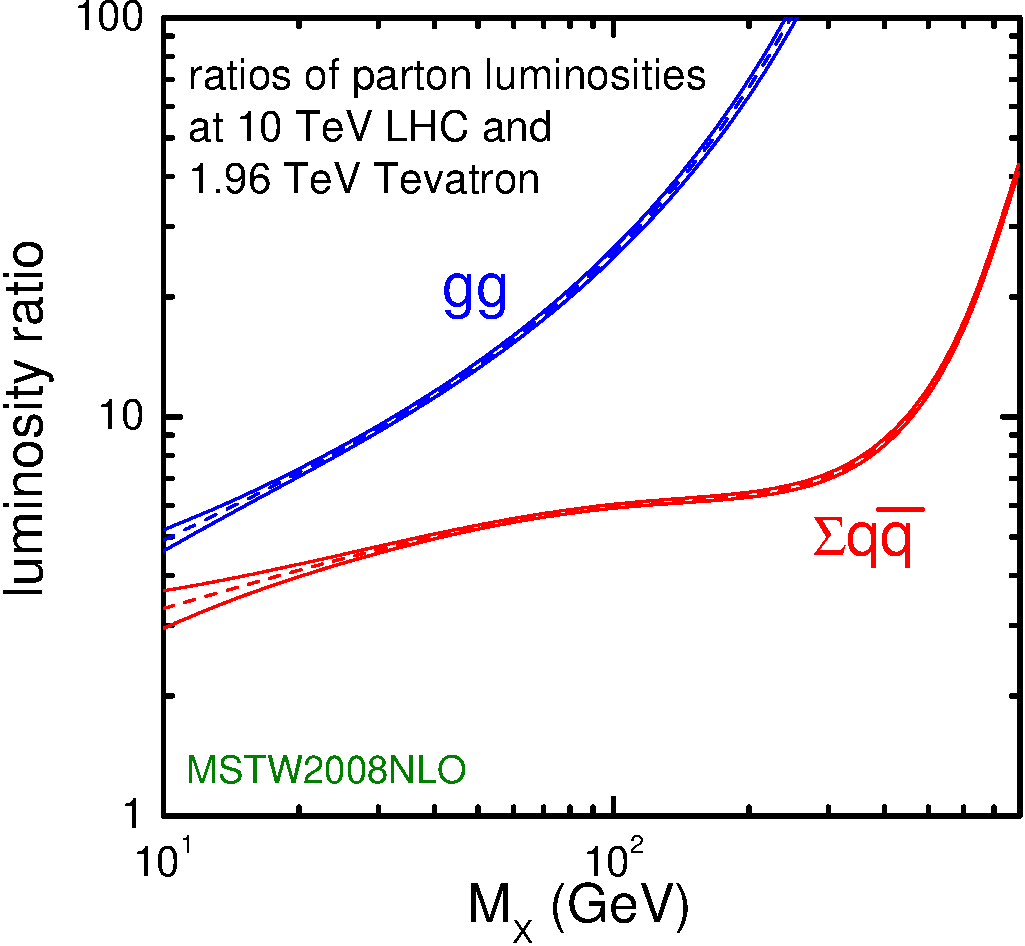
\includegraphics[width=90mm,angle=0]{theory_chapter/figures/parton_lumis_10TeV_vs_2TeV.pdf}
  \caption[Parton luminosity comparison of the LHC and Tevatron]{Ratio of the
  parton luminosity (the amount of luminosity contributed by the different
  species that compose the proton) of the LHC (at \mbox{$\sqrt s = 10~\TeV$}) and the
  Tevatron.  The large increase in gluon--gluon luminosity affects the favored
  production mechanisms of the Higgs boson.  } \label{fig:GluonLumiRatio}
\end{figure}
\begin{figure}
  \centering
  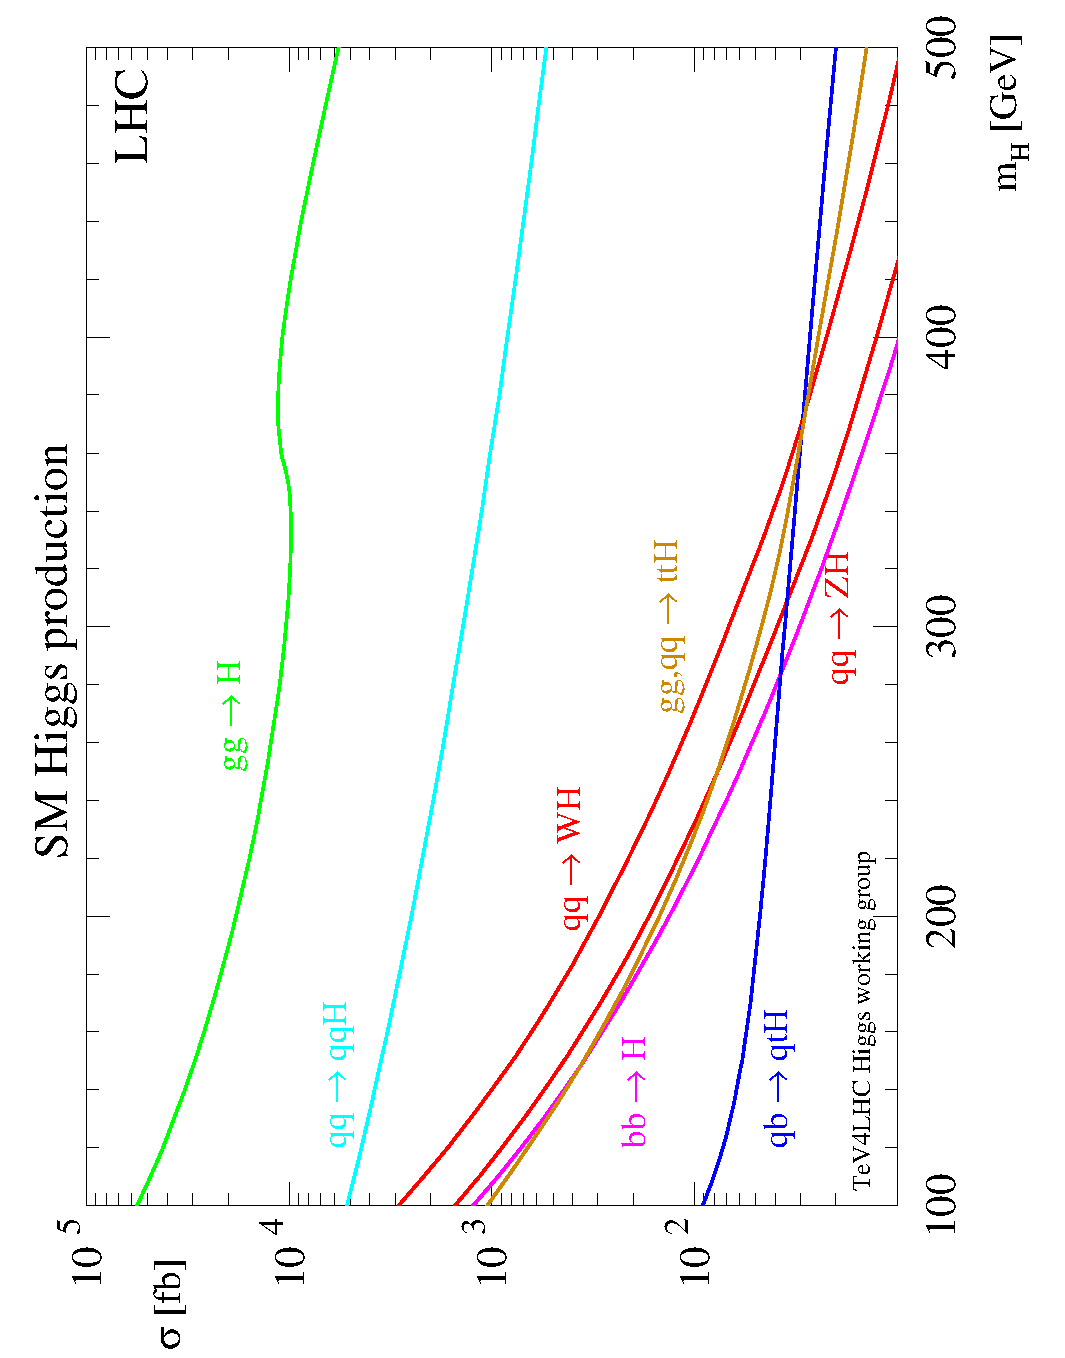
\includegraphics[width=90mm,angle=270]{theory_chapter/figures/lhcxs_mh.pdf}
  \caption[SM Higgs boson cross sections at the LHC]{Cross section of the SM Higgs
  boson versus the Higgs boson mass.  The different curves give the contribution
  to the cross section from different production mechanisms.
  Source:~\cite{PDG}.} \label{fig:LHCSMHiggsXsec}
\end{figure}

The branching fractions of the different decay modes of the SM Higgs boson
depend strongly on the mass of the Higgs boson.  In general, the Higgs prefers
(due to the Yukawa couplings) to decay pairs of the particles with the highest
mass possible.  Below the threshold to decay to pairs of weak bosons ($M_H <
160 \GeVcc$), the Higgs boson decays predominantly to either $b$--quarks (\bbbar,
90\%) or a pair of $\tau$ leptons (\TT, $\approx 10\%$).  Above the $W^\pm W^\mp$
threshold, decays to vector bosons ($H \to W^\pm W^\mp$ and $H \to ZZ$)
dominate.  The dependence of branching fraction on $M_H$ and the other rare
decay modes are illustrated in Figure~\ref{fig:SMHiggsBR}.  
\begin{figure}
  \centering
  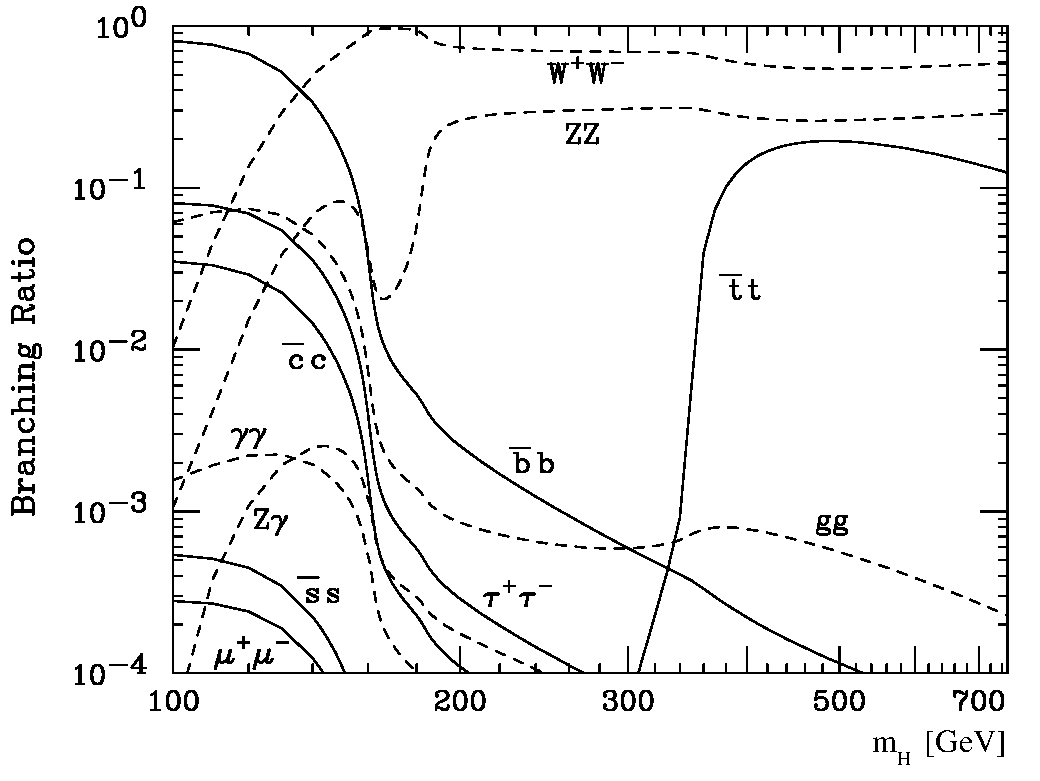
\includegraphics[width=90mm,angle=0]{theory_chapter/figures/smhiggsbr2_mh.pdf}
  \caption[SM Higgs boson branching fractions]{Branching fraction of the SM Higgs
  bosons for different values of $M_H$. Source:~\cite{PDG}.}
  \label{fig:SMHiggsBR}
\end{figure}
For low mass Higgs bosons,
the \TT decay mode plays a particularly important role.  The dominant decay mode
$H \to \bbbar$ suffers from enormous backgrounds from QCD jet production.
It is important to understand the magnitude of difference between expected Higgs
boson production and the rates of various backgrounds.
\begin{figure}
  \centering
  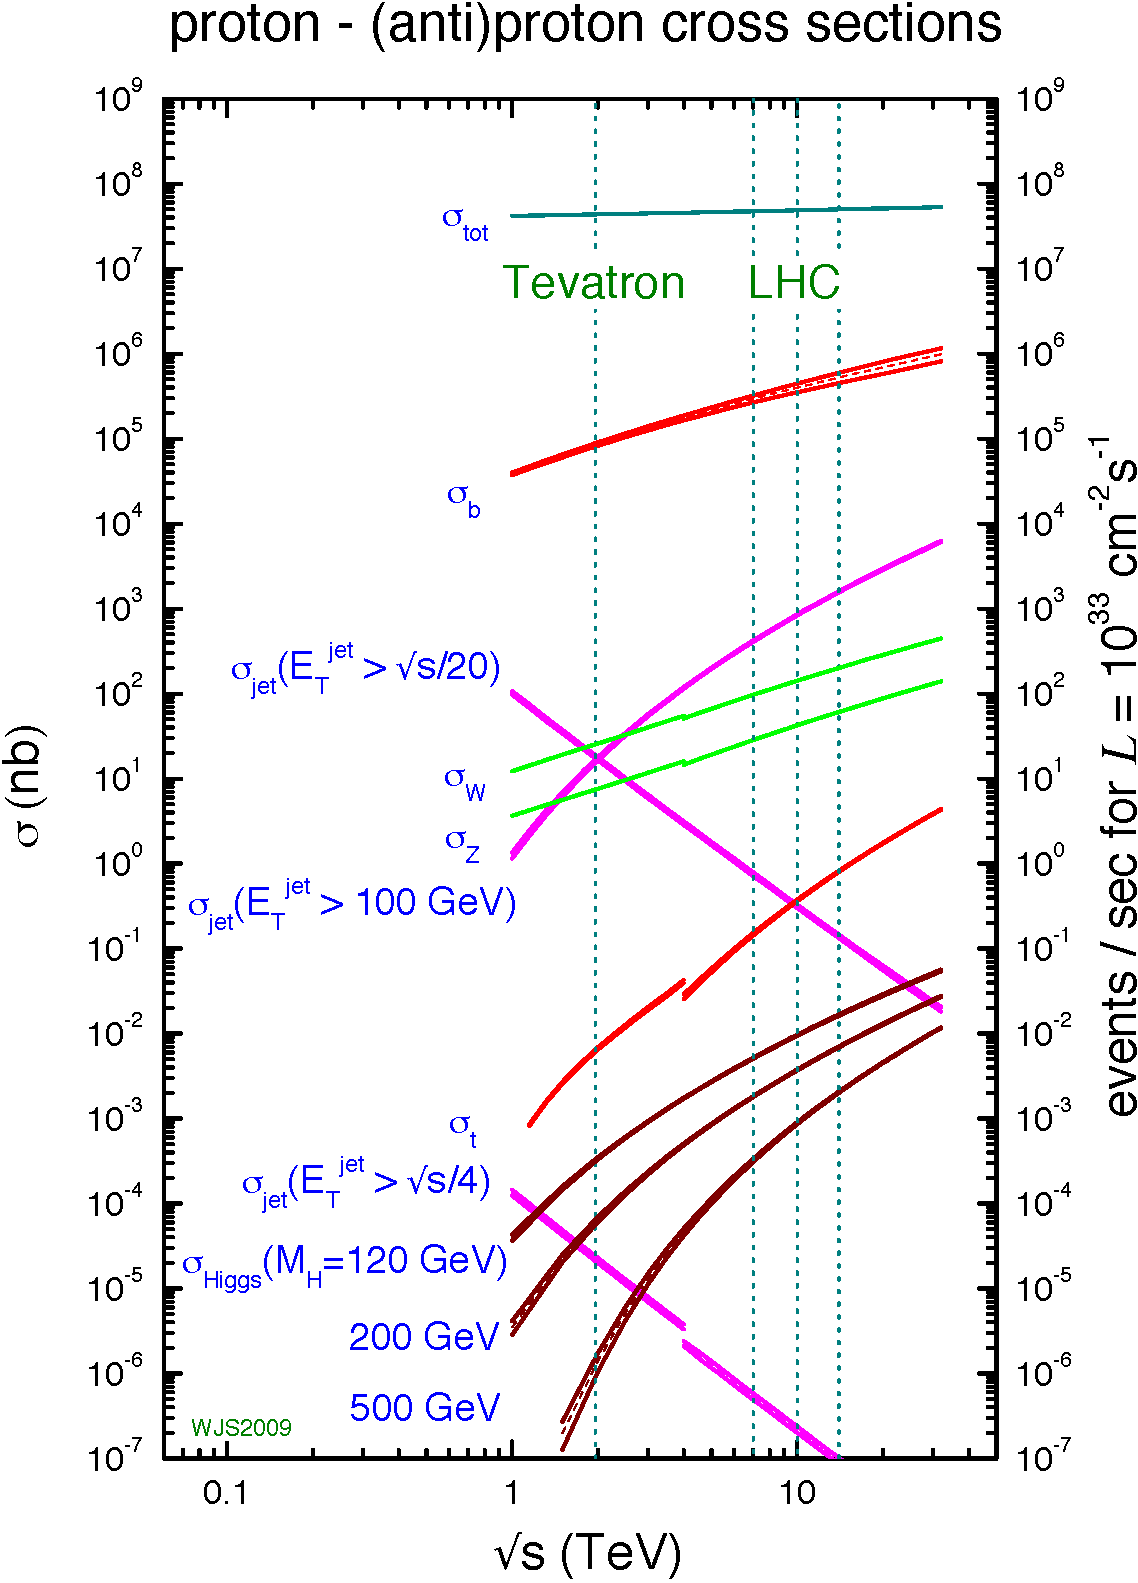
\includegraphics[width=100mm,angle=00]{theory_chapter/figures/collider_crosssections.pdf}
  \caption[Cross sections of interest at hadron colliders]{Cross sections of
  various processes at hadron colliders.  The horizontal axis represents the
  center of mass energy of the collision.  Of note is the vast difference in
  scales between Higgs boson production (maroon lines, $\bigO{10^{-2}~\text{nb}}$) and the QCD
  cross section to produce \bbbar pairs (red line, $\bigO{10^4~\text{nb}}$).
  Source:~\cite{MSTWXSectionPlots}.} 
  \label{fig:HadronColliderCrossSections}
\end{figure}
Figure~\ref{fig:HadronColliderCrossSections} illustrates the cross sections for
different SM processes at hadron colliders.  The rate of Higgs boson production is
many orders of magnitude ($\bigO{10^{-7}}$) smaller than that of QCD production.  It
is important to therefore design searches to use handles that can reject the
vast majority of the uninteresting events at hadron colliders.  

\subsection{MSSM Higgs Boson Phenomenology}
\label{sec:MSSMHiggsPhenom} The phenomenology of the Higgs sector of the MSSM is
similar to the SM in some respects, but differs in some key aspects which have
important implications for final states involving $\tau$ leptons and $b$ quarks.
When the parameter \tanb is large, the coupling factor between the Higgs bosons and the
down--type quarks and leptons (effectively the $\tau$ and $b$ quark) is enhanced
by $\tan\beta$.  The gluon--gluon cross section is therefore increased by
$\tan^2\beta$, where the top quark loop in Figure~\ref{fig:GluonFusion} is
replaced by a (\tanb enhanced) $b$ quark loop.  Additionally, MSSM Higgs
production with associated $b$--quarks, illustrated in
Figure~\ref{fig:AssociatedBProduction}, becomes an important production mode. 
\begin{figure}
  \centering
  \begin{fmffile}{AssociatedBProduction}
  \begin{fmfgraph*}(250,200)
    \fmfbottom{P1,P2} \fmftop{P1',b1,H',b2,P2'}
    \fmf{fermion,tension=2,lab=$P_1$}{P1,g1}
    \fmf{fermion,tension=2,lab=$P_2$}{P2,g2}
    \fmfblob{.16w}{g1,g2}
    \fmf{gluon,lab.side=right}{g1,v1}
    \fmf{gluon,lab.side=right}{v2,g2}
    \fmf{fermion,tension=.6}{b1,H,v1,v2,b2}
    \fmfdot{H,v1,v2}
    \fmf{dashes,lab=$H$,tension=0}{H,H'}
    \fmf{fermion}{g1,P1'}
    \fmf{fermion}{g2,P2'}
    \fmfv{lab=$g(x_1,,Q^2)$,lab.dist=.1w}{g1}
    \fmfv{lab=$g(x_2,,Q^2)$,lab.dist=.1w}{g2}
    \fmflabel{$\overline b$}{b1}
    \fmflabel{$b$}{b2}
    \fmffreeze
    \renewcommand{\P}[3]{\fmfi{plain}{%
    vpath(__#1,__#2) shifted (thick*(#3))}}
    \P{P1}{g1}{2,0} \P{P1}{g1}{-2,1}
    \P{P2}{g2}{2,1} \P{P2}{g2}{-2,0}
    \P{g1}{P1'}{-2,-1} \P{g1}{P1'}{2,0}
    \P{g2}{P2'}{-2,0} \P{g2}{P2'}{2,-1}
  \end{fmfgraph*}
  \end{fmffile}
  \label{fig:AssociatedBProduction} \caption[MSSM Higgs boson production with
  association $b$--quarks]{One possible diagram for an MSSM Higgs boson produced with
  associated $b$--quarks in a proton--proton collision.}
\end{figure}
At tree--level, the MSSM can be defined by the mass of the CP--odd Higgs boson \ma and
\tanb.  For a reasonably high \tanb, there is always one CP--even Higgs boson ($h^0$
or $H^0$) which is mass--degenerate with the $A^0$.  When \tanb and \ma are both
large, associated $b$ production dominates the total cross section~\cite{LHCHiggsXSecGroup}. The cross sections of the different MSSM
neutral Higgs bosons are shown in Figure~\ref{fig:MSSMXSectionsTanBeta}.
\begin{figure}
  \centering
  \subfigure[]{\includegraphics*[width=0.47\textwidth,angle=00]{theory_chapter/figures/YRHXS_MSSM_neutral_fig6a.pdf}
  \label{fig:MSSMXSectionsTanBeta5}
  }
  \subfigure[]{\includegraphics*[width=0.47\textwidth,angle=00]{theory_chapter/figures/YRHXS_MSSM_neutral_fig6b.pdf}
  \label{fig:MSSMXSectionsTanBeta30}
  }
  \caption[MSSM Higgs boson cross sections at the LHC]{Cross sections for the
  different MSSM Higgs bosons versus \ma in the $m_{h^{max}}$ benchmark
  scenario~\cite{MHMaxBenchmark} scenario for
  $\tanb=5$~\subref{fig:MSSMXSectionsTanBeta5} and
  $\tanb=30$~\subref{fig:MSSMXSectionsTanBeta30}.  Source:~\cite{LHCHiggsXSecGroup}
  }
  \label{fig:MSSMXSectionsTanBeta}
\end{figure}
The \tanb enhancement of the MSSM Higgs boson coupling to the $b$ quarks and $\tau$
leptons causes the branching fraction of all neutral MSSM Higgs states to be
$H\to\bbbar$~(90\%) and $H\to\TT$~(10\%) across the entire range of \ma.  The
enhanced production rate and the high branching fraction to $\tau$ leptons make
the MSSM Higgs bosons decaying to $\tau$ leptons an exciting and promising channel to
search for Higgs bosons and supersymmetric physics at colliders.

\subsection{Results from LEP and Tevatron}
\label{sec:lepAndTevatron}
The LEP and Tevatron experiments have both set limits on the existence of the
SM and MSSM Higgs boson.  Precision electroweak measurements
give additional hints on the prospects for both models.

LEP was an $e^+e^-$ collider at CERN and has effectively excluded the presence
of a low (less than $114~\GeVcc$) mass Higgs boson.  The dominant SM Higgs boson
production mode at LEP is Higgstrahlung, where the Higgs boson is produced in
association with a $Z$ boson (see Figure~\ref{fig:HiggsStrahlung}).  The search
at LEP utilized a number of different decay channels~\cite{PDG}.  The decay
channels used in the LEP search are summarized in Table~\ref{tab:LEPModes}.
\begin{table}
   \centering
   \begin{tabular}{|c|c|}
     \hline
     Higgs Decay & $Z$ Decay \\
     \hline
     \bbbar & \qqbar \\
     \TT & \qqbar \\
     \bbbar & \ttbar \\
     \bbbar & \nunubar \\
     \bbbar & \MM \\
     \bbbar & \EE \\
     \hline
   \end{tabular}
   \label{tab:LEPModes} 
   \caption[Higgs boson search channels at LEP]{Different channels used at LEP to
   search for Higgs bosons produced with the Higgstrahlung mechanism.}
\end{table}

The results using all channels from the four LEP experiments\footnote{ALEPH,
DELPHI, L3, and OPAL} have been combined into a single limit, shown in
Figure~\ref{fig:LEPHiggsLimit}.  The analysis sets a limit on the ratio $\xi^2 =
(g_\text{HZZ}/g_\text{HZZ})^2$, the upper limit on the HZZ coupling divided by
the predicted value of the SM\@.  For Higgs boson masses below $114~\GeVcc$, the
ratio is below unity at the 95\% confidence level, ruling out a SM
Higgs boson below that mass.
\begin{figure}
  \centering
  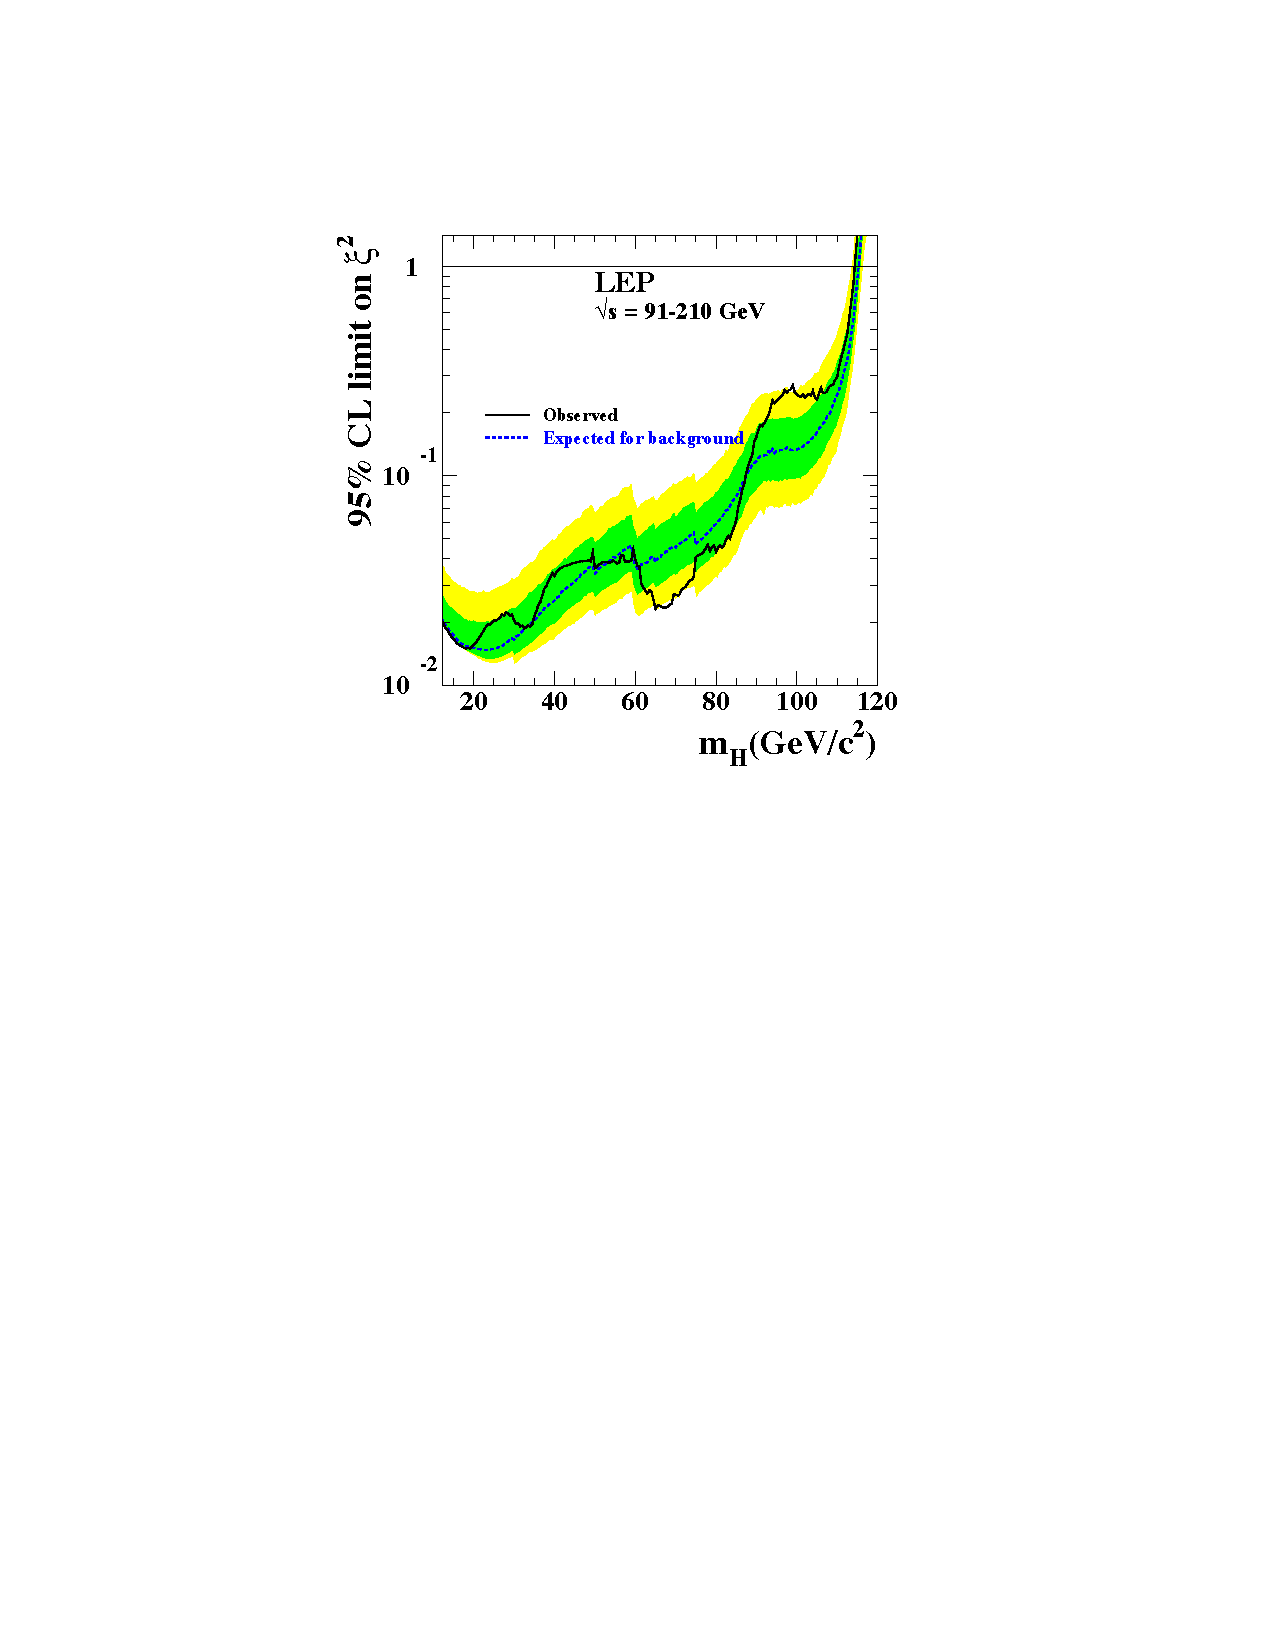
\includegraphics[width=100mm,angle=00]{theory_chapter/figures/lep_sm_limit.pdf}
  \caption[LEP SM Higgs boson limit plot]{Combined LEP upper limit set on the quantity
  \mbox{$\xi^2 = (g_\text{HZZ}/g_\text{HZZ})^2$} at 95\% confidence level.
  Regions where the observed ratio is less than one exclude the SM\@. The dashed
  line gives the expected limit for the null (background only) hypothesis, with
  the green and yellow bands representing the expected variance at one and two
  sigma, respectively, of the limit.  The solid line is the observed limit from
  the combined LEP data. Reference:~\cite{PDG} } \label{fig:LEPHiggsLimit}
\end{figure}

The Tevatron is a proton--antiproton collider with a center--of--mass energy of
$\sqrt s = 1.96~\TeV$.  There are two general purpose detectors at the Tevatron,
CDF and \DZERO\@. The dominant Higgs boson production modes at the Tevatron are
Higgstrahlung and gluon fusion (see Figure~\ref{fig:GluonFusion}).  For low mass
\mbox{($m_H < 135~\GeVcc$)} Higgs bosons the dominant channel at the Tevatron is
the Higgstrahlung production mode and \mbox{$H\to\bbbar$} decays.  Large
multi--jet backgrounds prevent the \mbox{$H\to\bbbar$} decay mode from being
useful for searching for Higgs bosons produced by gluon fusion.  The $H\to\TT$
and $H \to \gamma \gamma$ decays are additionally used in an inclusive search at
low mass, but do not dominate the search sensitivity.  The combined low--mass
limit on the SM Higgs boson from both Tevatron experiments is shown in
Figure~\ref{fig:TevatronLowMassHiggsLimit}.  The Tevatron currently sets an
upper limit on the SM Higgs boson cross section of about 2.5 times the SM
expectation.
\begin{figure}
  \centering
  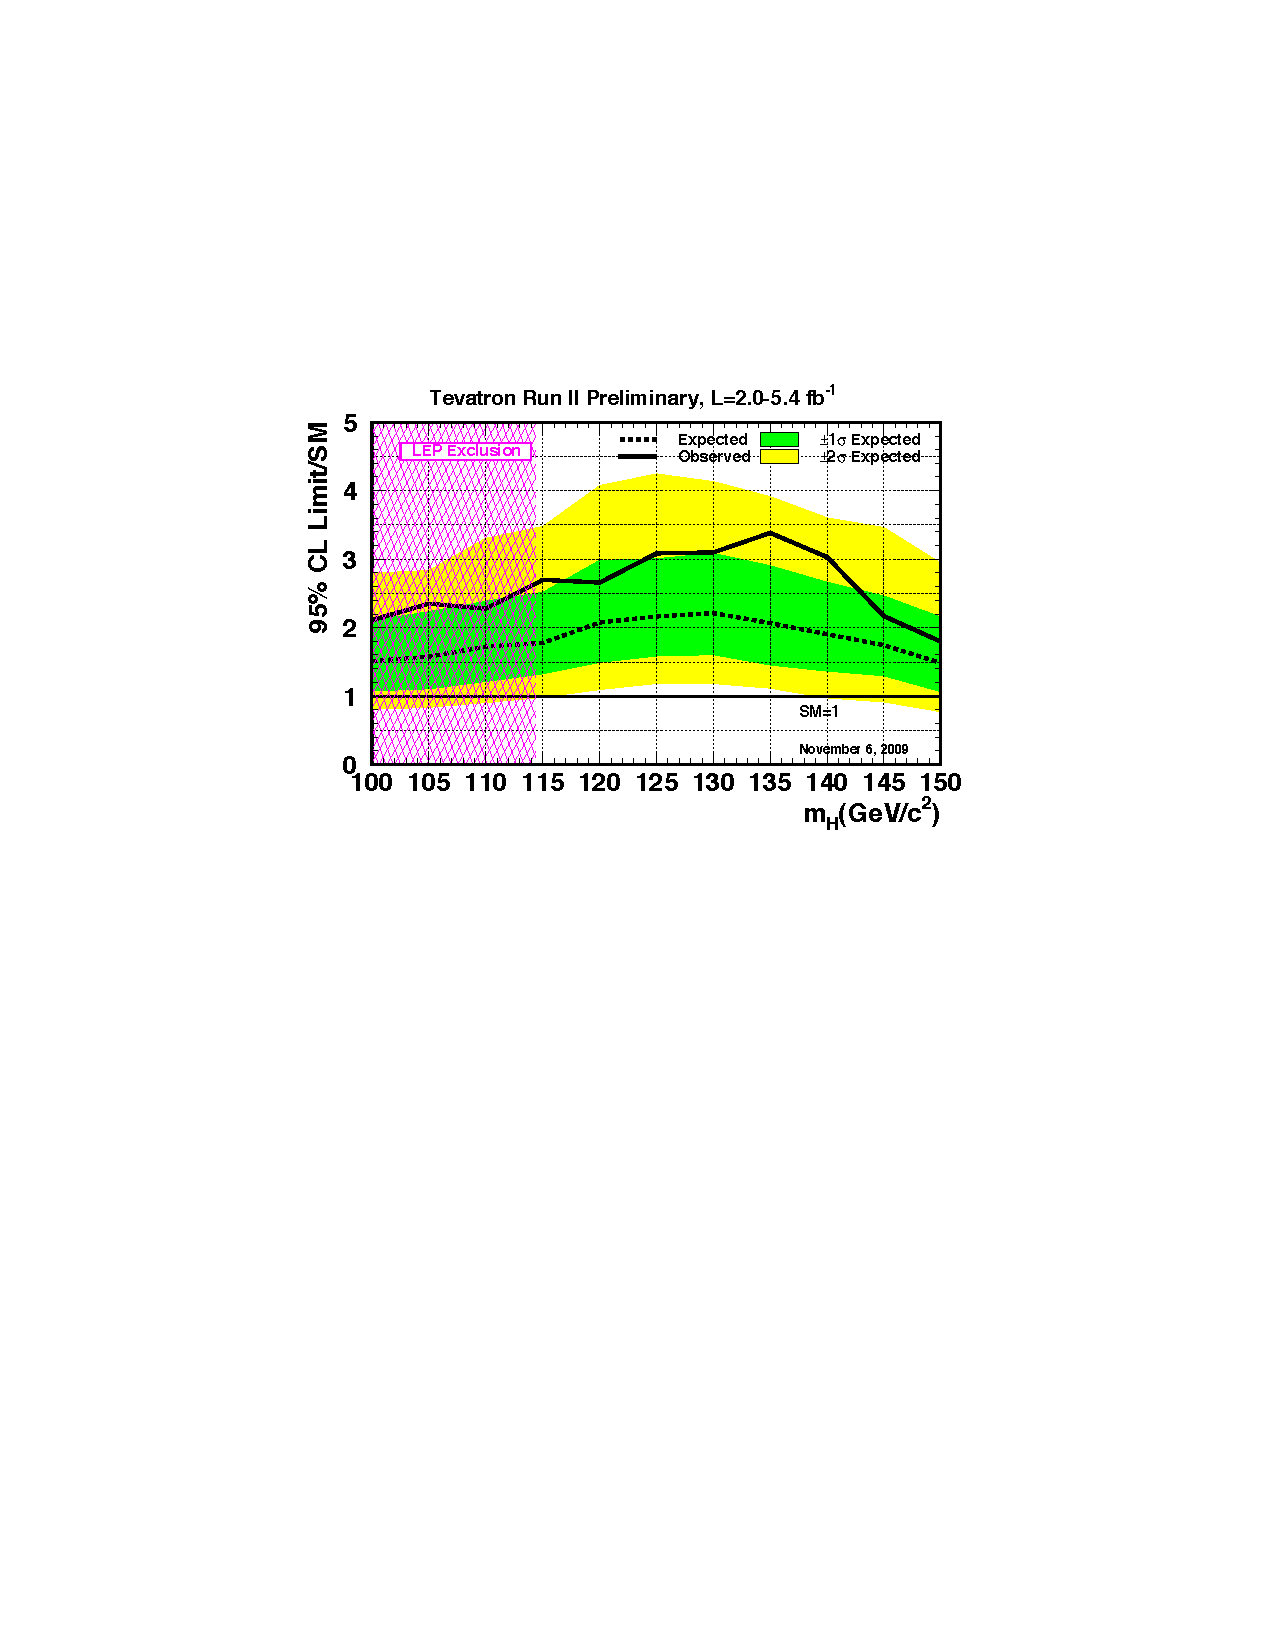
\includegraphics[height=100mm,angle=00]{theory_chapter/figures/tevatron_low_mass_sm_higgs_limit.pdf}
  \caption[Tevatron low mass standard model Higgs boson limit plot]{Combined CDF and
  \DZERO RunII upper limit on the cross section of a standard model--like Higgs
  boson.  The LEP limit is shown in pink. Reference:~\cite{PDG}}
  \label{fig:TevatronLowMassHiggsLimit}
\end{figure}

When \mbox{($m_H < 135~\GeVcc$)} the $H\to W^{+} W^{-}$ decay mode becomes
significant.  Low di--boson backgrounds allow this decay mode to probe both the
Higgstrahlung and gluon fusion production modes. The combined results of the CDF
and \DZERO searches using the $W^+W^-$ have decay mode recently excluded (See
Figure~\ref{fig:TevatronHighMassHiggsLimit}) a SM Higgs boson with a mass
between 162 and 166~\GeVcc.  This is the first exclusion in SM Higgs boson
mass parameter space since the LEP result.
\begin{figure}
  \centering
  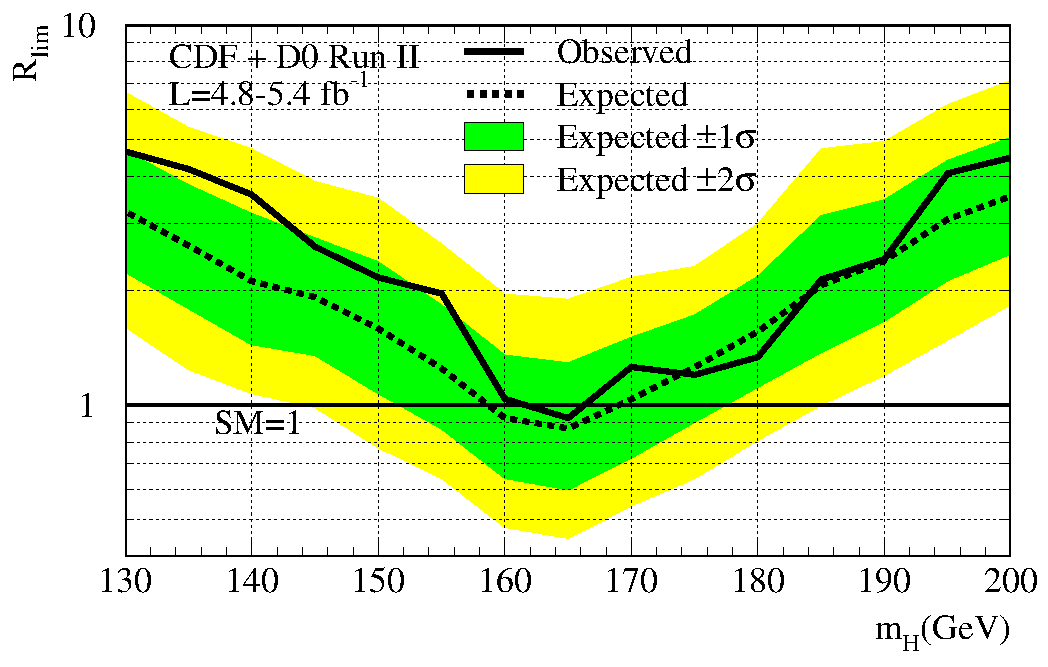
\includegraphics[width=0.75\textwidth]{theory_chapter/figures/tevwwlimits.pdf}
  \caption[Tevatron high mass standard model Higgs boson limit plot]{Combined CDF and
  \DZERO RunII upper limit on the cross section of a SM--like Higgs
  boson using the $H \to W^+W^-$ decay mode.  The SM is excluded for
  Higgs boson masses between 162 and 166~\GeVcc. Reference:~\cite{PDG}}
  \label{fig:TevatronHighMassHiggsLimit}
\end{figure}

Analyses at LEP and Tevatron have also addressed excluded regions of the MSSM\@.
At LEP, the dominant production modes of the MSSM Higgs bosons are Higgstrahlung
and pair production, where $e^+e^- \to h^0 A^0$ or $H^0 A^0$.  For the
Higgstrahlung production mode, the SM search can be reinterpreted in
terms of the MSSM\@.  To address the pair production mode, searches were
performed in the $e^+e^- \to h^0 A^0 \to \bbbar \bbbar$ and $\TT \qqbar$ decay
modes.  Finally, LEP is also sensitive to associated MSSM Higgs boson production at
low $\ma$ and high $\tan\beta$ to $\EE \to {\cal f}\overline{\cal f} \phi$,
where the associated fermions ${\cal f}$ are \mbox{$b$--quarks} or tau leptons.
The combined limits from LEP in the \mbox{$\ma--\tan\beta$} plane are shown in
Figure~\ref{fig:LEPMSSMLimits}.
\begin{figure}
  \centering
  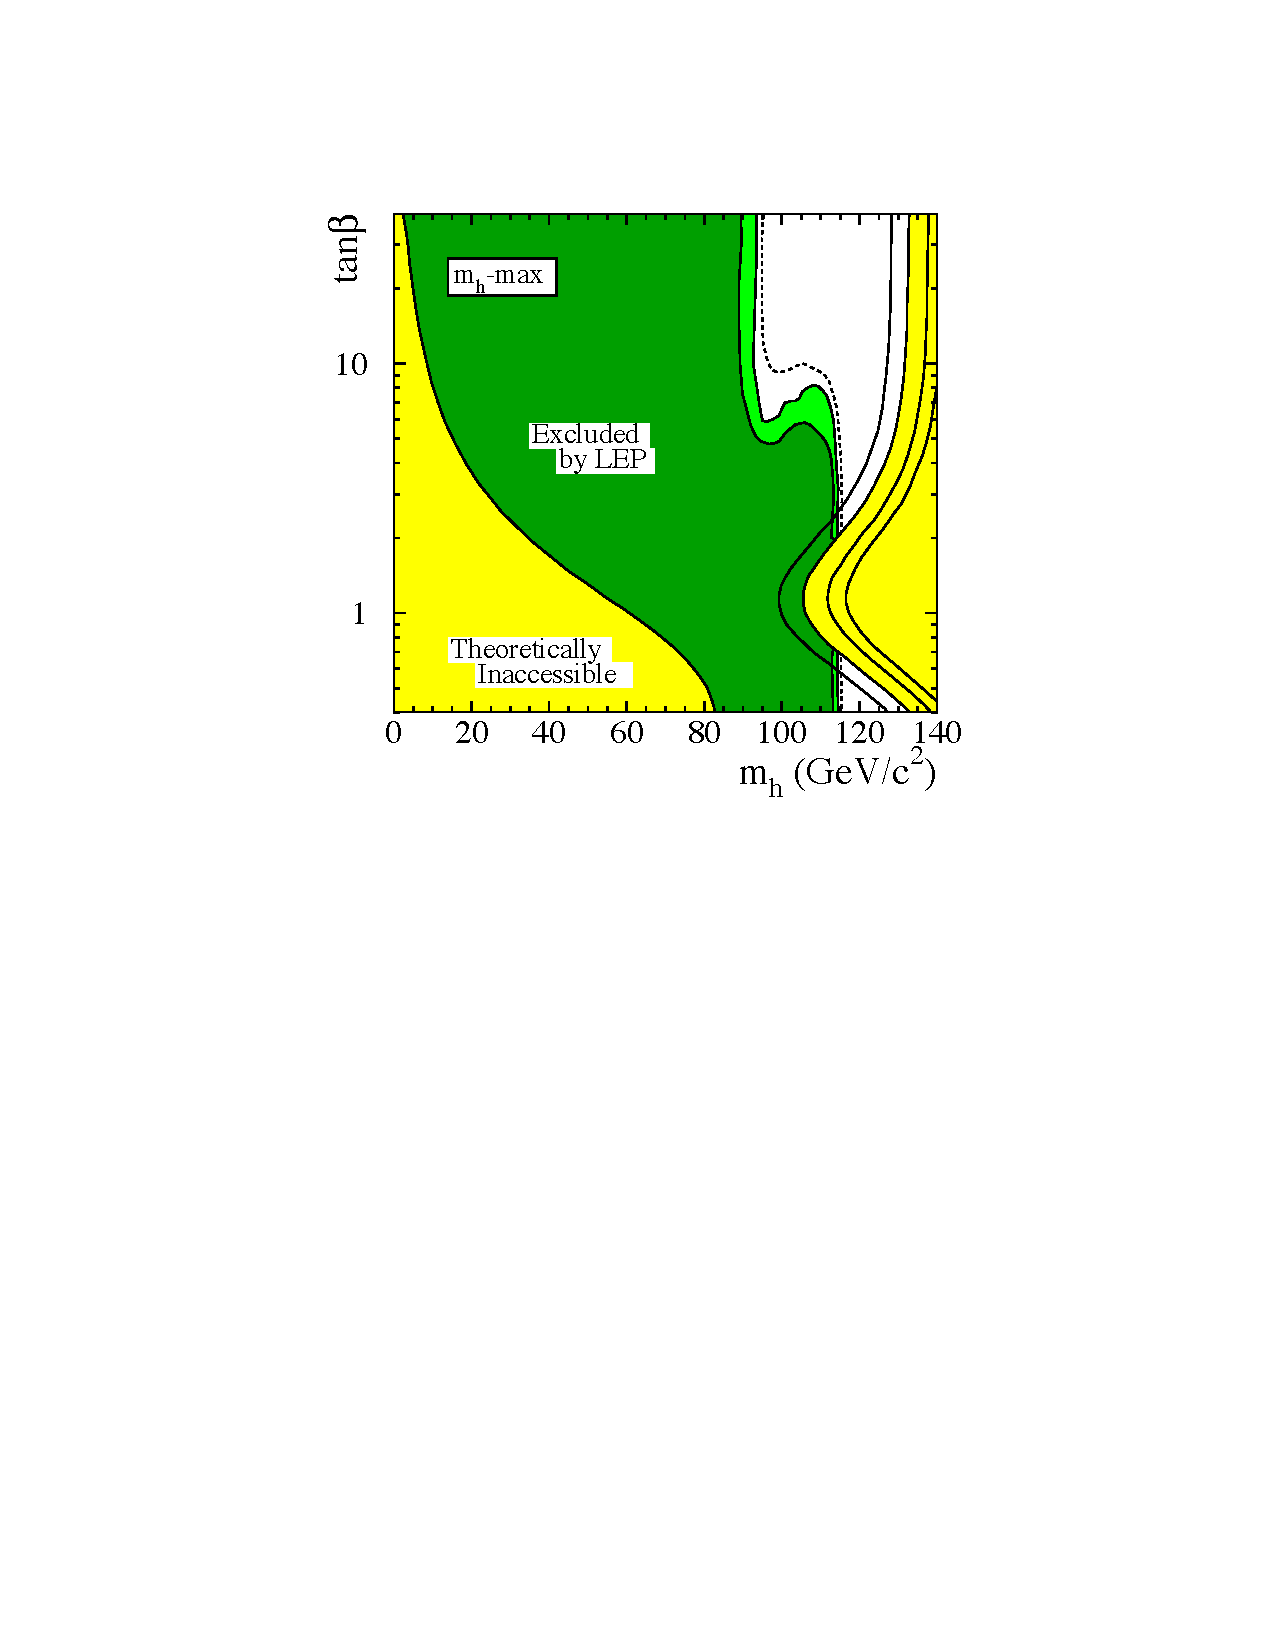
\includegraphics[width=0.75\textwidth]{theory_chapter/figures/lep_mssm_exclusion.pdf}
  \caption[LEP MSSM exclusion limits]{Combined LEP limits on the MSSM\@.  The
  results are interpreted in the context of the \mbox{$m_h$--max}
  benchmark~\cite{MHMaxBenchmark} scenario of the MSSM\@.  Reference:~\cite{PDG}}
  \label{fig:LEPMSSMLimits}
\end{figure}

At the Tevatron, CDF and \DZERO have set a combined limit on the MSSM using the
inclusive $H\to\TT$ channel.  The analysis presented in this thesis is very  
similar to the approaches used at the Tevatron.  Results from the Tevatron have
excluded the MSSM for $\tan\beta$ greater than approximately 35 for MSSM Higgs
boson mass $\ma < 200~\GeVcc$.   The full
exclusion plot for the \mbox{$m_h$--max} and ``no mixing'' MSSM benchmark
scenarios are shown in Figure~\ref{fig:TevMSSMLimits}.
\begin{figure}
  \centering
  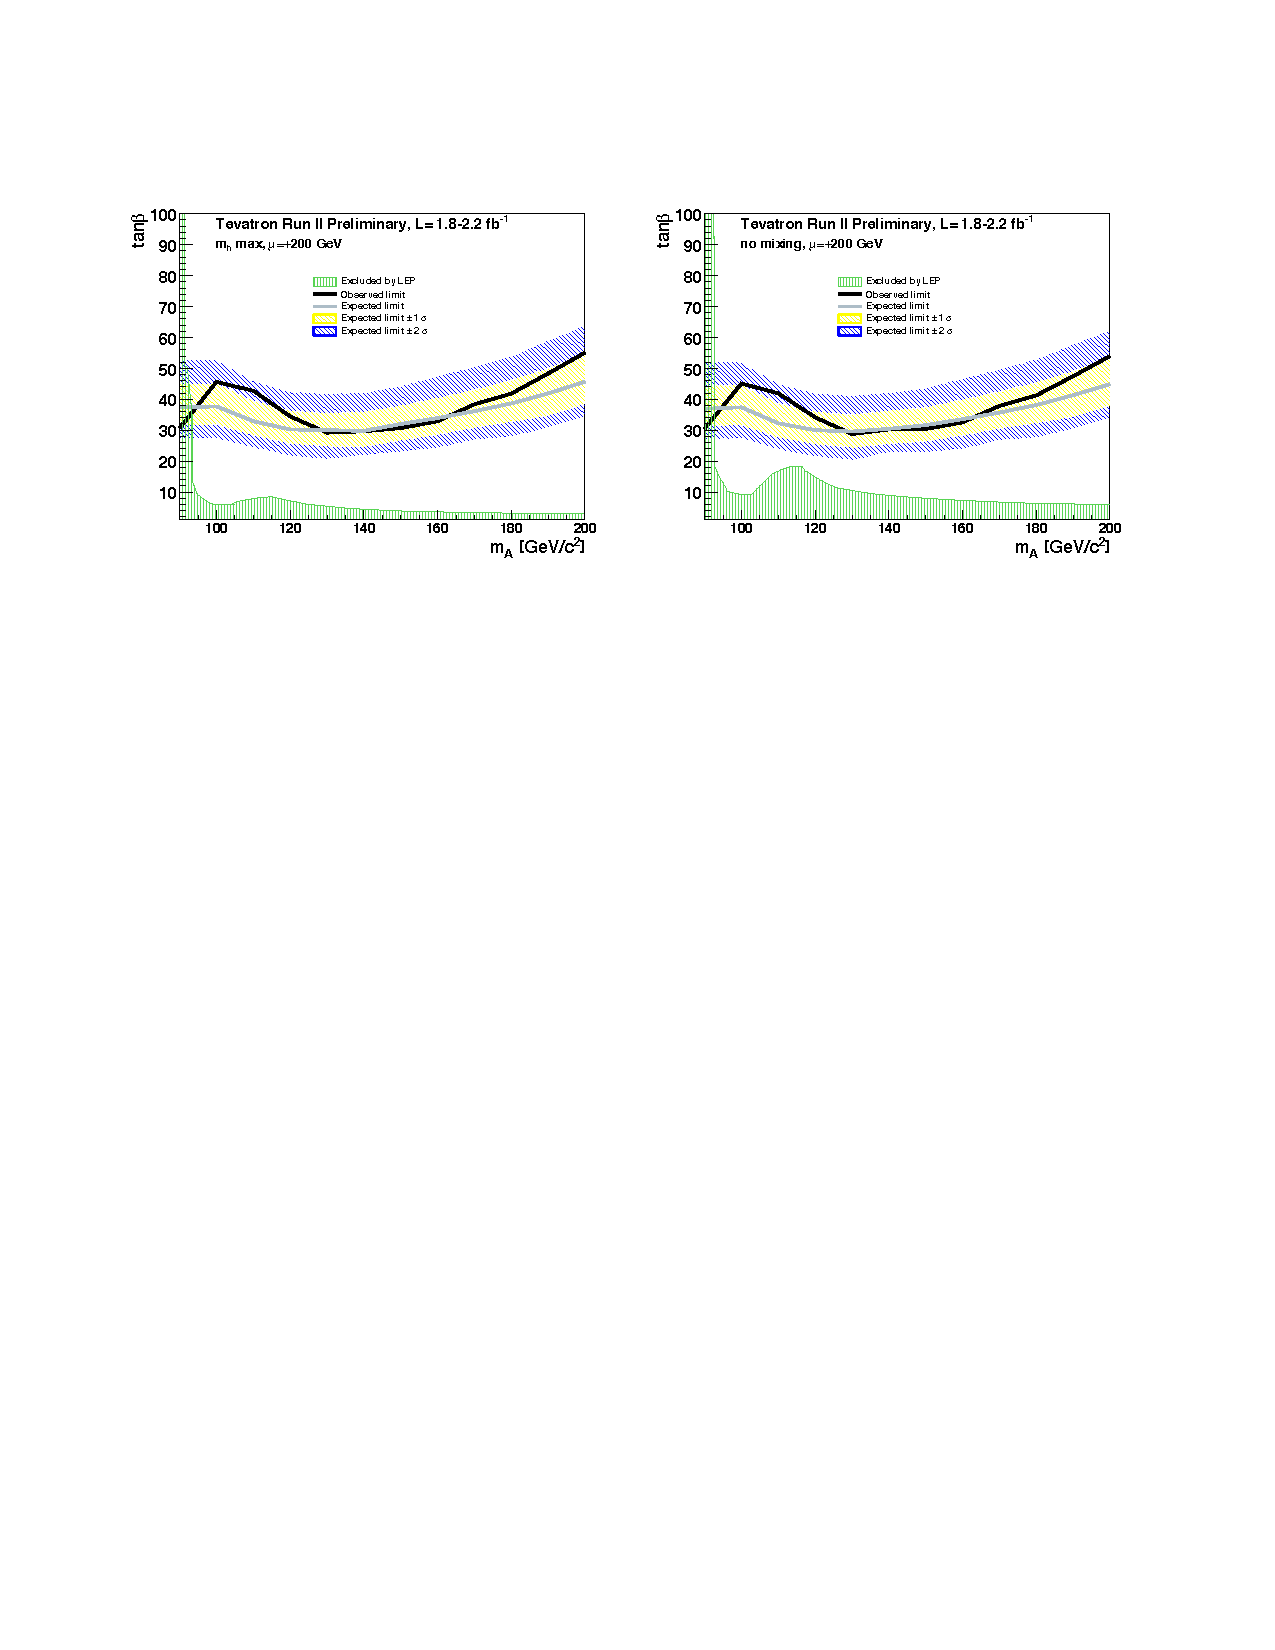
\includegraphics[width=0.99\textwidth]{theory_chapter/figures/tev_mssm_limits_mhmax_and_nomixing.pdf}
  \caption[Tevatron MSSM exclusion limits]{Combined Tevatron limits on the
  MSSM\@.  The grey line and blue and yellow bands gives the expected limit and
  its one and two sigma contours.  The black line is the observed limit.
  The results are interpreted in the context of the \mbox{$m_h$--max}
  benchmark (left) and ``no mixing'' (right) MSSM scenarios.  The limit from LEP
  is shown in green.
  Reference:~\cite{PDG}} \label{fig:TevMSSMLimits}
\end{figure}

\section{The Physics of the Tau Lepton}
As discussed in Sections~\ref{sec:SMHiggsPhenom} and~\ref{sec:MSSMAndTaus}, the
$\tau$ lepton is an important probe of Higgs physics.  The \taul has some
unusual properties which make it particularly challenging at hadron colliders.
With a mass of 1.78~\GeVcc, the \taul is heaviest of the leptons.  The nominal
decay distance $c\tau$ of the \taul is 87~\micron, which in practice means that
the $\tau$ will always decay before reaching the first layer of the detector.
Tau decays can be effectively classified into two types. ``Leptonic'' decays
consist of a $\tau$ decaying to a light lepton ($\ell = e, \mu$) and two
neutrinos $\tau^+ \to \ell^+ \nu_\tau \overline{ \nu_{\ell}}$.  ``Hadronic''
decays consist of a low--multiplicity collimated group of hadrons, typically
\Pgppm~and \Pgpz~mesons.  The hadronic decays of the \taul compose approximately
$65\%$ of the \taul branching fraction, with the remainder shared approximately
equally by the leptonic decays.  The branching fractions for the leptonic and
most common hadronic decays are shown in Table~\ref{tab:decay_modes}.
\begin{table}
   \centering
   \begin{tabular}{lccc}
      Visible Decay Products  & Resonance & Mass (\MeVcc) &
      Fraction~\cite{PDG} \\
      \hline
      \hline
      \multicolumn{4}{c}{Leptonic modes} \\
      \hline
      $e^- \nu_\tau \overline \nu_e$             & -      & 0.5  & 17.8\% \\
      $\mu^-\nu_\tau \overline \nu_\mu$          & -      & 105  & 17.4\% \\
      \hline
      \multicolumn{4}{c}{Hadronic modes} \\
      \hline
      $\pi^{-} \nu_\tau$                    & -      & 135  & 10.9\% \\
      $\pi^{-}\pi^0 \nu_\tau$               & $\rho$ & 770  & 25.5\% \\
      $\pi^{-}\pi^0\pi^0 \nu_\tau$          & $a1$   & 1200 & 9.3\% \\
      $\pi^{-}\pi^{-}\pi^{+} \nu_\tau$      & $a1$   & 1200 & 9.0\% \\
      $\pi^{-}\pi^{-}\pi^{+}\pi^0 \nu_\tau$ & $a1$   & 1200 & 4.5\% \\
      \hline
      Total                                 &        &      & 94.4\% \\
      \hline
   \end{tabular}
   \label{tab:decay_modes} \caption[Decay modes of the $\tau$ lepton]{Resonances
   and branching ratios of the dominant decay modes of the \taul.  The decay
   products listed correspond to a negatively charged \taul; the table is
   identical under charge conjugation.}
\end{table}

The tau is also a challenging object in that the decay of the tau always
includes neutrinos.  The associated neutrinos are weakly interacting and do not
create a signal in any detector at CMS\@.  The only sign that the neutrinos are
there is an imbalance in the total transverse\footnote{At proton colliders, the
constituent quarks/gluons of the proton share the total proton momentum.  As the
total fraction of momentum carried by the parton involved in a hard collision is
unknown, longitudinal momentum is not conserved.} energy in the event.  This
thesis will describe a novel way to reconstruct the neutrinos associated to tau
decays in Chapter~\ref{ch:svfit}.  

A tau with produced with energy $E$ travels on average 
\begin{equation}
  \gamma c \tau = \frac{E}{1.78~\GeV} 87~\micro\meter \nonumber
\end{equation}
before decaying in the detector.  These lengths are comparable to the resolution
of the CMS tracker, therefore it is possible to reconstruct a vertex
corresponding to a tau decay that is displaced with respect to the primary
vertex.  This can be used as an additional discriminant against QCD, which is
expected to decay promptly.  Furthermore, in Chapter~\ref{ch:svfit} we will see
it may be possible to use it when reconstructing the associated neutrinos.

\ifx\master\undefined% AUTOCOMPILE
% Allows for individual chapters to be compiled.

% Usage:
% \ifx\master\undefined% AUTOCOMPILE
% Allows for individual chapters to be compiled.

% Usage:
% \ifx\master\undefined% AUTOCOMPILE
% Allows for individual chapters to be compiled.

% Usage:
% \ifx\master\undefined\input{../settings/autocompile}\fi
% (place at start and end of chapter file)

\ifx\noprelim\undefined
    % first time included
    % input preamble files
    \input{../settings/phdsetup}

    \begin{document}
    \def\noprelim{}
\else
    % already included once
    % input post files

    \singlespacing
    \bibliographystyle{../bibliography/expanded}
    \bibliography{../bibliography/references}

    \end{document}
\fi\fi
% (place at start and end of chapter file)

\ifx\noprelim\undefined
    % first time included
    % input preamble files
    % [ USER VARIABLES ]

\def\PHDTITLE {Extensions of the Theory of Computational Mechanics}
\def\PHDAUTHOR{Evan Klose Friis}
\def\PHDSCHOOL{University of California, Davis}

\def\PHDMONTH {June}
\def\PHDYEAR  {2011}
\def\PHDDEPT {Physics}

\def\BSSCHOOL {University of California at San Diego}
\def\BSYEAR   {2005}

\def\PHDCOMMITTEEA{Professor John Conway}
\def\PHDCOMMITTEEB{Professor Robin Erbacher}
\def\PHDCOMMITTEEC{Professor Mani Tripathi}

% [ GLOBAL SETUP ]

\documentclass[letterpaper,oneside,11pt]{report}

\usepackage{calc}
\usepackage{breakcites}
\usepackage[newcommands]{ragged2e}

\usepackage[pdftex]{graphicx}
\usepackage{epstopdf}

%\usepackage{tikz}
%\usetikzlibrary{positioning} % [right=of ...]
%\usetikzlibrary{fit} % [fit= ...]

%\pgfdeclarelayer{background layer}
%\pgfdeclarelayer{foreground layer}
%\pgfsetlayers{background layer,main,foreground layer}

%\newenvironment{wrap}{\noindent\begin{minipage}[t]{\linewidth}\vspace{-0.5\normalbaselineskip}\centering}{\vspace{0.5\normalbaselineskip}\end{minipage}}

%% [Venn diagram environment]
%\newenvironment{venn2}
%{\begin{tikzpicture} [every pin/.style={text=black, text opacity=1.0, pin distance=0.5cm, pin edge={black!60, semithick}},
%% define a new style 'venn'
%venn/.style={circle, draw=black!60, semithick, minimum size = 4cm}]
%
%% create circle and give it external (pin) label
%\node[venn] (X) at (-1,0) [pin={150:$H[X]$}] {};
%\node[venn] (Y) at (1,0) [pin={30:$H[Y]$}] {};
%
%% place labels of the atoms by hand
%\node at (-1.9,0) {$H[X|Y]$};
%\node at (1.9,0) {$H[Y|X]$};
%\node at (0,0) {$I[X;Y]$};}
%{\end{tikzpicture}}

%\newcommand{\wrapmath}[1]{\begin{wrap}\begin{tikzpicture}[every node/.style={inner ysep=0ex, inner xsep=0em}]\node[] {$\displaystyle\begin{aligned} #1\end{aligned}$};\end{tikzpicture}\end{wrap}}

\renewenvironment{abstract}{\chapter*{Abstract}}{}
\renewcommand{\bibname}{Bibliography}
\renewcommand{\contentsname}{Table of Contents}

\makeatletter
\renewcommand{\@biblabel}[1]{\textsc{#1}}
\makeatother

% [ FONT SETTINGS ]

\usepackage[tbtags, intlimits, namelimits]{amsmath}
\usepackage[adobe-utopia]{mathdesign}

\DeclareSymbolFont{pazomath}{OMS}{zplm}{m}{n}
\DeclareSymbolFontAlphabet{\mathcal}{pazomath}
\SetMathAlphabet\mathcal{bold}{OMS}{zplm}{b}{n}

\SetSymbolFont{largesymbols}{normal}{OMX}{zplm}{m}{n}
\SetSymbolFont{largesymbols}{bold}{OMX}{zplm}{m}{n}
\SetSymbolFont{symbols}{normal}{OMS}{zplm}{m}{n}
\SetSymbolFont{symbols}{bold}{OMS}{zplm}{b}{n}

\renewcommand{\sfdefault}{phv}
\renewcommand{\ttdefault}{fvm}

\widowpenalty 8000
\clubpenalty  8000

% [ PAGE LAYOUT ]
\usepackage{geometry}
\geometry{lmargin = 1.5in}
\geometry{rmargin = 1.0in}
\geometry{tmargin = 1.0in}
\geometry{bmargin = 1.0in}

% [ PDF SETTINGS ]

\usepackage[final]{hyperref}
\hypersetup{breaklinks  = true}
\hypersetup{colorlinks  = true}
\hypersetup{linktocpage = false}
\hypersetup{linkcolor   = blue}
\hypersetup{citecolor   = green}
\hypersetup{urlcolor    = black}
\hypersetup{plainpages  = false}
\hypersetup{pageanchor  = true}
\hypersetup{pdfauthor   = {\PHDAUTHOR}}
\hypersetup{pdftitle    = {\PHDTITLE}}
\hypersetup{pdfsubject  = {Dissertation, \PHDSCHOOL}}
\urlstyle{same}

% [ LETTER SPACING ]

\usepackage[final]{microtype}
\microtypesetup{protrusion=compatibility}
\microtypesetup{expansion=false}

\newcommand{\upper}[1]{\MakeUppercase{#1}}
\let\lsscshape\scshape

\ifcase\pdfoutput\else\microtypesetup{letterspace=15}
\renewcommand{\scshape}{\lsscshape\lsstyle}
\renewcommand{\upper}[1]{\textls[50]{\MakeUppercase{#1}}}\fi

% [ LINE SPACING ]

\usepackage[doublespacing]{setspace}
\renewcommand{\displayskipstretch}{0.0}

\setlength{\parskip   }{0em}
\setlength{\parindent }{2em}

% [ TABLE FORMATTING ]

\usepackage{booktabs}
\setlength{\heavyrulewidth}{1.5\arrayrulewidth}
\setlength{\lightrulewidth}{1.0\arrayrulewidth}
\setlength{\doublerulesep }{2.0\arrayrulewidth}

% [ SECTION FORMATTING ]

\usepackage[largestsep,nobottomtitles*]{titlesec}
\renewcommand{\bottomtitlespace}{0.75in}

\titleformat{\chapter}[display]{\bfseries\huge\singlespacing}{\filleft\textsc{\LARGE \chaptertitlename\ \thechapter}}{-0.2ex}{\titlerule[3pt]\vspace{0.2ex}}[]

\titleformat{\section}{\LARGE}{\S\thesection\hspace{0.5em}}{0ex}{}
\titleformat{\subsection}{\Large}{\S\thesubsection\hspace{0.5em}}{0ex}{}
\titleformat{\subsubsection}{\large}{\thesubsubsection\hspace{0.5em}}{0ex}{}

\titlespacing*{\chapter}{0em}{6ex}{4ex plus 2ex minus 0ex}
\titlespacing*{\section}{0em}{2ex plus 3ex minus 1ex}{0.5ex plus 0.5ex minus 0.5ex}
\titlespacing*{\subsection}{0ex}{2ex plus 3ex minus 1ex}{0ex}
\titlespacing*{\subsubsection}{0ex}{2ex plus 0ex minus 1ex}{0ex}

% [ HEADER SETTINGS ]

\usepackage{fancyhdr}

\setlength{\headheight}{\normalbaselineskip}
\setlength{\footskip  }{0.5in}
\setlength{\headsep   }{0.5in-\headheight}

\fancyheadoffset[R]{0.5in}
\renewcommand{\headrulewidth}{0pt}
\renewcommand{\footrulewidth}{0pt}

\newcommand{\pagebox}{\parbox[r][\headheight][t]{0.5in}{\hspace\fill\thepage}}

\newcommand{\prelimheaders}{\ifx\prelim\undefined\renewcommand{\thepage}{\textit{\roman{page}}}\fancypagestyle{plain}{\fancyhf{}\fancyfoot[L]{\makebox[\textwidth-0.5in]{\thepage}}}\pagestyle{plain}\def\prelim{}\fi}

\newcommand{\normalheaders}{\renewcommand{\thepage}{\arabic{page}}\fancypagestyle{plain}{\fancyhf{}\fancyhead[R]{\pagebox}}\pagestyle{plain}}

\normalheaders{}

% [ CUSTOM COMMANDS ]

\newcommand{\signaturebox}[1]{\multicolumn{1}{p{4in}}{\vspace{3ex}}\\\midrule #1\\}

%\input{../includes/cmechabbrev}

% [some math stuff - maybe stick in sep file]
\usepackage{amsthm}
\usepackage{amscd}
\theoremstyle{plain}    \newtheorem{Lem}{Lemma}
\theoremstyle{plain}    \newtheorem*{ProLem}{Proof}
\theoremstyle{plain} 	\newtheorem{Cor}{Corollary}
\theoremstyle{plain} 	\newtheorem*{ProCor}{Proof}
\theoremstyle{plain} 	\newtheorem{The}{Theorem}
\theoremstyle{plain} 	\newtheorem*{ProThe}{Proof}
\theoremstyle{plain} 	\newtheorem{Prop}{Proposition}
\theoremstyle{plain} 	\newtheorem*{ProProp}{Proof}
\theoremstyle{plain} 	\newtheorem*{Conj}{Conjecture}
\theoremstyle{plain}	\newtheorem*{Rem}{Remark}
\theoremstyle{plain}	\newtheorem*{Def}{Definition} 
\theoremstyle{plain}	\newtheorem*{Not}{Notation}

% [uniform figure scaling - maybe this is not a good idea]
\def\figscale{.7}
\def\lscale{1.0}

% [FIX ME! - red makes it easier to spot]
\newcommand{\FIX}[1]{\textbf{\textcolor{red}{#1}}}


    \begin{document}
    \def\noprelim{}
\else
    % already included once
    % input post files

    \singlespacing
    \bibliographystyle{../bibliography/expanded}
    \bibliography{../bibliography/references}

    \end{document}
\fi\fi
% (place at start and end of chapter file)

\ifx\noprelim\undefined
    % first time included
    % input preamble files
    % [ USER VARIABLES ]

\def\PHDTITLE {Extensions of the Theory of Computational Mechanics}
\def\PHDAUTHOR{Evan Klose Friis}
\def\PHDSCHOOL{University of California, Davis}

\def\PHDMONTH {June}
\def\PHDYEAR  {2011}
\def\PHDDEPT {Physics}

\def\BSSCHOOL {University of California at San Diego}
\def\BSYEAR   {2005}

\def\PHDCOMMITTEEA{Professor John Conway}
\def\PHDCOMMITTEEB{Professor Robin Erbacher}
\def\PHDCOMMITTEEC{Professor Mani Tripathi}

% [ GLOBAL SETUP ]

\documentclass[letterpaper,oneside,11pt]{report}

\usepackage{calc}
\usepackage{breakcites}
\usepackage[newcommands]{ragged2e}

\usepackage[pdftex]{graphicx}
\usepackage{epstopdf}

%\usepackage{tikz}
%\usetikzlibrary{positioning} % [right=of ...]
%\usetikzlibrary{fit} % [fit= ...]

%\pgfdeclarelayer{background layer}
%\pgfdeclarelayer{foreground layer}
%\pgfsetlayers{background layer,main,foreground layer}

%\newenvironment{wrap}{\noindent\begin{minipage}[t]{\linewidth}\vspace{-0.5\normalbaselineskip}\centering}{\vspace{0.5\normalbaselineskip}\end{minipage}}

%% [Venn diagram environment]
%\newenvironment{venn2}
%{\begin{tikzpicture} [every pin/.style={text=black, text opacity=1.0, pin distance=0.5cm, pin edge={black!60, semithick}},
%% define a new style 'venn'
%venn/.style={circle, draw=black!60, semithick, minimum size = 4cm}]
%
%% create circle and give it external (pin) label
%\node[venn] (X) at (-1,0) [pin={150:$H[X]$}] {};
%\node[venn] (Y) at (1,0) [pin={30:$H[Y]$}] {};
%
%% place labels of the atoms by hand
%\node at (-1.9,0) {$H[X|Y]$};
%\node at (1.9,0) {$H[Y|X]$};
%\node at (0,0) {$I[X;Y]$};}
%{\end{tikzpicture}}

%\newcommand{\wrapmath}[1]{\begin{wrap}\begin{tikzpicture}[every node/.style={inner ysep=0ex, inner xsep=0em}]\node[] {$\displaystyle\begin{aligned} #1\end{aligned}$};\end{tikzpicture}\end{wrap}}

\renewenvironment{abstract}{\chapter*{Abstract}}{}
\renewcommand{\bibname}{Bibliography}
\renewcommand{\contentsname}{Table of Contents}

\makeatletter
\renewcommand{\@biblabel}[1]{\textsc{#1}}
\makeatother

% [ FONT SETTINGS ]

\usepackage[tbtags, intlimits, namelimits]{amsmath}
\usepackage[adobe-utopia]{mathdesign}

\DeclareSymbolFont{pazomath}{OMS}{zplm}{m}{n}
\DeclareSymbolFontAlphabet{\mathcal}{pazomath}
\SetMathAlphabet\mathcal{bold}{OMS}{zplm}{b}{n}

\SetSymbolFont{largesymbols}{normal}{OMX}{zplm}{m}{n}
\SetSymbolFont{largesymbols}{bold}{OMX}{zplm}{m}{n}
\SetSymbolFont{symbols}{normal}{OMS}{zplm}{m}{n}
\SetSymbolFont{symbols}{bold}{OMS}{zplm}{b}{n}

\renewcommand{\sfdefault}{phv}
\renewcommand{\ttdefault}{fvm}

\widowpenalty 8000
\clubpenalty  8000

% [ PAGE LAYOUT ]
\usepackage{geometry}
\geometry{lmargin = 1.5in}
\geometry{rmargin = 1.0in}
\geometry{tmargin = 1.0in}
\geometry{bmargin = 1.0in}

% [ PDF SETTINGS ]

\usepackage[final]{hyperref}
\hypersetup{breaklinks  = true}
\hypersetup{colorlinks  = true}
\hypersetup{linktocpage = false}
\hypersetup{linkcolor   = blue}
\hypersetup{citecolor   = green}
\hypersetup{urlcolor    = black}
\hypersetup{plainpages  = false}
\hypersetup{pageanchor  = true}
\hypersetup{pdfauthor   = {\PHDAUTHOR}}
\hypersetup{pdftitle    = {\PHDTITLE}}
\hypersetup{pdfsubject  = {Dissertation, \PHDSCHOOL}}
\urlstyle{same}

% [ LETTER SPACING ]

\usepackage[final]{microtype}
\microtypesetup{protrusion=compatibility}
\microtypesetup{expansion=false}

\newcommand{\upper}[1]{\MakeUppercase{#1}}
\let\lsscshape\scshape

\ifcase\pdfoutput\else\microtypesetup{letterspace=15}
\renewcommand{\scshape}{\lsscshape\lsstyle}
\renewcommand{\upper}[1]{\textls[50]{\MakeUppercase{#1}}}\fi

% [ LINE SPACING ]

\usepackage[doublespacing]{setspace}
\renewcommand{\displayskipstretch}{0.0}

\setlength{\parskip   }{0em}
\setlength{\parindent }{2em}

% [ TABLE FORMATTING ]

\usepackage{booktabs}
\setlength{\heavyrulewidth}{1.5\arrayrulewidth}
\setlength{\lightrulewidth}{1.0\arrayrulewidth}
\setlength{\doublerulesep }{2.0\arrayrulewidth}

% [ SECTION FORMATTING ]

\usepackage[largestsep,nobottomtitles*]{titlesec}
\renewcommand{\bottomtitlespace}{0.75in}

\titleformat{\chapter}[display]{\bfseries\huge\singlespacing}{\filleft\textsc{\LARGE \chaptertitlename\ \thechapter}}{-0.2ex}{\titlerule[3pt]\vspace{0.2ex}}[]

\titleformat{\section}{\LARGE}{\S\thesection\hspace{0.5em}}{0ex}{}
\titleformat{\subsection}{\Large}{\S\thesubsection\hspace{0.5em}}{0ex}{}
\titleformat{\subsubsection}{\large}{\thesubsubsection\hspace{0.5em}}{0ex}{}

\titlespacing*{\chapter}{0em}{6ex}{4ex plus 2ex minus 0ex}
\titlespacing*{\section}{0em}{2ex plus 3ex minus 1ex}{0.5ex plus 0.5ex minus 0.5ex}
\titlespacing*{\subsection}{0ex}{2ex plus 3ex minus 1ex}{0ex}
\titlespacing*{\subsubsection}{0ex}{2ex plus 0ex minus 1ex}{0ex}

% [ HEADER SETTINGS ]

\usepackage{fancyhdr}

\setlength{\headheight}{\normalbaselineskip}
\setlength{\footskip  }{0.5in}
\setlength{\headsep   }{0.5in-\headheight}

\fancyheadoffset[R]{0.5in}
\renewcommand{\headrulewidth}{0pt}
\renewcommand{\footrulewidth}{0pt}

\newcommand{\pagebox}{\parbox[r][\headheight][t]{0.5in}{\hspace\fill\thepage}}

\newcommand{\prelimheaders}{\ifx\prelim\undefined\renewcommand{\thepage}{\textit{\roman{page}}}\fancypagestyle{plain}{\fancyhf{}\fancyfoot[L]{\makebox[\textwidth-0.5in]{\thepage}}}\pagestyle{plain}\def\prelim{}\fi}

\newcommand{\normalheaders}{\renewcommand{\thepage}{\arabic{page}}\fancypagestyle{plain}{\fancyhf{}\fancyhead[R]{\pagebox}}\pagestyle{plain}}

\normalheaders{}

% [ CUSTOM COMMANDS ]

\newcommand{\signaturebox}[1]{\multicolumn{1}{p{4in}}{\vspace{3ex}}\\\midrule #1\\}

%%%% macros fro standard references
%\eqref provided by amsmath
\newcommand{\figref}[1]{Fig.~\ref{#1}}
\newcommand{\tableref}[1]{Table~\ref{#1}}
\newcommand{\refcite}[1]{Ref.~\cite{#1}}

% Abbreviations from CMPPSS:

\newcommand{\eM}     {\mbox{$\epsilon$-machine}}
\newcommand{\eMs}    {\mbox{$\epsilon$-machines}}
\newcommand{\EM}     {\mbox{$\epsilon$-Machine}}
\newcommand{\EMs}    {\mbox{$\epsilon$-Machines}}
\newcommand{\eT}     {\mbox{$\epsilon$-transducer}}
\newcommand{\eTs}    {\mbox{$\epsilon$-transducers}}
\newcommand{\ET}     {\mbox{$\epsilon$-Transducer}}
\newcommand{\ETs}    {\mbox{$\epsilon$-Transducers}}

% Processes and sequences

\newcommand{\Process}{\mathcal{P}}

\newcommand{\ProbMach}{\Prob_{\mathrm{M}}}
\newcommand{\Lmax}   { {L_{\mathrm{max}}}}
\newcommand{\MeasAlphabet}	{\mathcal{A}}
% Original
%\newcommand{\MeasSymbol}   { {S} }
%\newcommand{\meassymbol}   { {s} }
% New symbol
\newcommand{\MeasSymbol}   { {X} }
\newcommand{\meassymbol}   { {x} }
\newcommand{\BiInfinity}	{ \overleftrightarrow {\MeasSymbol} }
\newcommand{\biinfinity}	{ \overleftrightarrow {\meassymbol} }
\newcommand{\Past}	{ \overleftarrow {\MeasSymbol} }
\newcommand{\past}	{ {\overleftarrow {\meassymbol}} }
\newcommand{\pastprime}	{ {\past}^{\prime}}
\newcommand{\Future}	{ \overrightarrow{\MeasSymbol} }
\newcommand{\future}	{ \overrightarrow{\meassymbol} }
\newcommand{\futureprime}	{ {\future}^{\prime}}
\newcommand{\PastPrime}	{ {\Past}^{\prime}}
\newcommand{\FuturePrime}	{ {\overrightarrow{\meassymbol}}^\prime }
\newcommand{\PastDblPrime}	{ {\overleftarrow{\meassymbol}}^{\prime\prime} }
\newcommand{\FutureDblPrime}	{ {\overrightarrow{\meassymbol}}^{\prime\prime} }
\newcommand{\pastL}	{ {\overleftarrow {\meassymbol}}{}^L }
\newcommand{\PastL}	{ {\overleftarrow {\MeasSymbol}}{}^L }
\newcommand{\PastLt}	{ {\overleftarrow {\MeasSymbol}}_t^L }
\newcommand{\PastLLessOne}	{ {\overleftarrow {\MeasSymbol}}^{L-1} }
\newcommand{\futureL}	{ {\overrightarrow{\meassymbol}}{}^L }
\newcommand{\FutureL}	{ {\overrightarrow{\MeasSymbol}}{}^L }
\newcommand{\FutureLt}	{ {\overrightarrow{\MeasSymbol}}_t^L }
\newcommand{\FutureLLessOne}	{ {\overrightarrow{\MeasSymbol}}^{L-1} }
\newcommand{\pastLprime}	{ {\overleftarrow {\meassymbol}}^{L^\prime} }
\newcommand{\futureLprime}	{ {\overrightarrow{\meassymbol}}^{L^\prime} }
\newcommand{\AllPasts}	{ { \overleftarrow {\rm {\bf \MeasSymbol}} } }
\newcommand{\AllFutures}	{ \overrightarrow {\rm {\bf \MeasSymbol}} }
\newcommand{\FutureSet}	{ \overrightarrow{\bf \MeasSymbol}}

% Causal states and epsilon-machines
\newcommand{\CausalState}	{ \mathcal{S} }
\newcommand{\CausalStatePrime}	{ {\CausalState}^{\prime}}
\newcommand{\causalstate}	{ \sigma }
\newcommand{\CausalStateSet}	{ \boldsymbol{\CausalState} }
\newcommand{\AlternateState}	{ \mathcal{R} }
\newcommand{\AlternateStatePrime}	{ {\cal R}^{\prime} }
\newcommand{\alternatestate}	{ \rho }
\newcommand{\alternatestateprime}	{ {\rho^{\prime}} }
\newcommand{\AlternateStateSet}	{ \boldsymbol{\AlternateState} }
\newcommand{\PrescientState}	{ \widehat{\AlternateState} }
\newcommand{\prescientstate}	{ \widehat{\alternatestate} }
\newcommand{\PrescientStateSet}	{ \boldsymbol{\PrescientState}}
\newcommand{\CausalEquivalence}	{ {\sim}_{\epsilon} }
\newcommand{\CausalEquivalenceNot}	{ {\not \sim}_{\epsilon}}

\newcommand{\NonCausalEquivalence}	{ {\sim}_{\eta} }
\newcommand{\NextObservable}	{ {\overrightarrow {\MeasSymbol}}^1 }
\newcommand{\LastObservable}	{ {\overleftarrow {\MeasSymbol}}^1 }
%\newcommand{\Prob}		{ {\rm P}}
\newcommand{\Prob}      {\Pr} % use standard command
\newcommand{\ProbAnd}	{ {,\;} }
\newcommand{\LLimit}	{ {L \rightarrow \infty}}
\newcommand{\Cmu}		{C_\mu}
\newcommand{\hmu}		{h_\mu}
\newcommand{\EE}		{{\bf E}}
\newcommand{\Measurable}{{\bf \mu}}

% Process Crypticity
\newcommand{\PC}		{\chi}
\newcommand{\FuturePC}		{\PC^+}
\newcommand{\PastPC}		{\PC^-}
% Causal Irreversibility
\newcommand{\CI}		{\Xi}
\newcommand{\ReverseMap}	{r}
\newcommand{\ForwardMap}	{f}

% Abbreviations from IB:
% None that aren't already in CMPPSS

% Abbreviations from Extensive Estimation:
\newcommand{\EstCausalState}	{\widehat{\CausalState}}
\newcommand{\estcausalstate}	{\widehat{\causalstate}}
\newcommand{\EstCausalStateSet}	{\boldsymbol{\EstCausalState}}
\newcommand{\EstCausalFunc}	{\widehat{\epsilon}}
\newcommand{\EstCmu}		{\widehat{\Cmu}}
\newcommand{\PastLOne}	{{\Past}^{L+1}}
\newcommand{\pastLOne}	{{\past}^{L+1}}

% Abbreviations from $\epsilon$-Transducers:
\newcommand{\InAlphabet}	{ \mathcal{A}}
\newcommand{\insymbol}		{ a}
\newcommand{\OutAlphabet}	{ \mathcal{B}}
\newcommand{\outsymbol}		{ b}
\newcommand{\InputSimple}	{ X}
\newcommand{\inputsimple}	{ x}
\newcommand{\BottleneckVar}	{\tilde{\InputSimple}}
\newcommand{\bottleneckvar}	{\tilde{\inputsimple}}
\newcommand{\InputSpace}	{ \mathbf{\InputSimple}}
\newcommand{\InputBi}	{ \overleftrightarrow {\InputSimple} }
\newcommand{\inputbi}	{ \overleftrightarrow {\inputsimple} }
\newcommand{\InputPast}	{ \overleftarrow {\InputSimple} }
\newcommand{\inputpast}	{ \overleftarrow {\inputsimple} }
\newcommand{\InputFuture}	{ \overrightarrow {\InputSimple} }
\newcommand{\inputfuture}	{ \overrightarrow {\inputsimple} }
\newcommand{\NextInput}	{ {{\InputFuture}^{1}}}
\newcommand{\NextOutput}	{ {\OutputFuture}^{1}}
\newcommand{\OutputSimple}	{ Y}
\newcommand{\outputsimple}	{ y}
\newcommand{\OutputSpace}	{ \mathbf{\OutputSimple}}
\newcommand{\OutputBi}	{ \overleftrightarrow{\OutputSimple} }
\newcommand{\outputbi}	{ \overleftrightarrow{\outputsimple} }
\newcommand{\OutputPast}	{ \overleftarrow{\OutputSimple} }
\newcommand{\outputpast}	{ \overleftarrow{\outputsimple} }
\newcommand{\OutputFuture}	{ \overrightarrow{\OutputSimple} }
\newcommand{\outputfuture}	{ \overrightarrow{\outputsimple} }
\newcommand{\OutputL}	{ {\OutputFuture}^L}
\newcommand{\outputL}	{ {\outputfuture}^L}
\newcommand{\InputLLessOne}	{ {\InputFuture}^{L-1}}
\newcommand{\inputLlessone}	{ {\inputufutre}^{L-1}}
\newcommand{\OutputPastLLessOne}	{{\OutputPast}^{L-1}_{-1}}
\newcommand{\outputpastLlessone}	{{\outputpast}^{L-1}}
\newcommand{\OutputPastLessOne}	{{\OutputPast}_{-1}}
\newcommand{\outputpastlessone}	{{\outputpast}_{-1}}
\newcommand{\OutputPastL}	{{\OutputPast}^{L}}
\newcommand{\OutputLPlusOne}	{ {\OutputFuture}^{L+1}}
\newcommand{\outputLplusone}	{ {\outputfutre}^{L+1}}
\newcommand{\InputPastL}	{{\InputPast}^{L}}
\newcommand{\inputpastL}	{{\inputpast}^{L}}
\newcommand{\JointPast}	{{(\InputPast,\OutputPast)}}
\newcommand{\jointpast}	{{(\inputpast,\outputpast)}}
\newcommand{\jointpastone}	{{(\inputpast_1,\outputpast_1)}}
\newcommand{\jointpasttwo}	{{(\inputpast_2,\outputpast_2)}}
\newcommand{\jointpastprime} {{({\inputpast}^{\prime},{\outputpast}^{\prime})}}
\newcommand{\NextJoint}	{{(\NextInput,\NextOutput)}}
\newcommand{\nextjoint}	{{(\insymbol,\outsymbol)}}
\newcommand{\AllInputPasts}	{ { \overleftarrow {\rm \InputSpace}}}
\newcommand{\AllOutputPasts}	{ {\overleftarrow {\rm \OutputSpace}}}
\newcommand{\DetCausalState}	{ {{\cal S}_D }}
\newcommand{\detcausalstate}	{ {{\sigma}_D} }
\newcommand{\DetCausalStateSet}	{ \boldsymbol{{\CausalState}_D}}
\newcommand{\DetCausalEquivalence}	{ {\sim}_{{\epsilon}_{D}}}
\newcommand{\PrescientEquivalence}	{ {\sim}_{\widehat{\eta}}}
\newcommand{\FeedbackCausalState}	{ \mathcal{F}}
\newcommand{\feedbackcausalstate}	{ \phi}
\newcommand{\FeedbackCausalStateSet}	{ \mathbf{\FeedbackCausalState}}
\newcommand{\JointCausalState}		{ \mathcal{J}}
\newcommand{\JointCausalStateSet}	{ \mathbf{\JointCausalState}}
\newcommand{\UtilityFunctional}	{ {\mathcal{L}}}
\newcommand{\NatureState}	{ {\Omega}}
\newcommand{\naturestate}	{ {\omega}}
\newcommand{\NatureStateSpace}	{ {\mathbf{\NatureState}}}
\newcommand{\AnAction}	{ {A}}
\newcommand{\anaction}	{ {a}}
\newcommand{\ActionSpace}	{ {\mathbf{\AnAction}}}

% Abbreviations from RURO:
\newcommand{\InfoGain}[2] { \mathcal{D} \left( {#1} || {#2} \right) }

% Abbreviations from Upper Bound:
\newcommand{\lcm}	{{\rm lcm}}
% Double-check that this isn't in the math set already!

% Abbreviations from Emergence in Space
\newcommand{\ProcessAlphabet}	{\MeasAlphabet}
\newcommand{\ProbEst}			{ {\widehat{\Prob}_N}}
\newcommand{\STRegion}			{ {\mathrm K}}
\newcommand{\STRegionVariable}		{ K}
\newcommand{\stregionvariable}		{ k}
\newcommand{\GlobalPast}		{ \overleftarrow{G}} 
\newcommand{\globalpast}		{ \overleftarrow{g}} 
\newcommand{\GlobalFuture}		{ \overrightarrow{G}}
\newcommand{\globalfuture}		{ \overrightarrow{g}}
\newcommand{\GlobalState}		{ \mathcal{G}}
\newcommand{\globalstate}		{ \gamma}
\newcommand{\GlobalStateSet}		{ {\mathbf \GlobalState}}
\newcommand{\LocalPast}			{ \overleftarrow{L}} 
\newcommand{\localpast}			{ \overleftarrow{l}}
\newcommand{\AllLocalPasts}		{ \mathbf{\LocalPast}}
\newcommand{\LocalPastRegion}		{ \overleftarrow{\mathrm L}}
\newcommand{\LocalFuture}		{ \overrightarrow{L}}
\newcommand{\localfuture}		{ \overrightarrow{l}}
\newcommand{\LocalFutureRegion}		{ \overrightarrow{\mathrm L}}
\newcommand{\LocalState}		{ \mathcal{L}}
\newcommand{\localstate}		{ \lambda}
\newcommand{\LocalStateSet}		{ {\mathbf \LocalState}}
\newcommand{\PatchPast}			{ \overleftarrow{P}}
\newcommand{\patchpast}			{ \overleftarrow{p}}
\newcommand{\PatchPastRegion}		{ \overleftarrow{\mathrm P}}
\newcommand{\PatchFuture}		{ \overrightarrow{P}}
\newcommand{\patchfuture}		{ \overrightarrow{p}}
\newcommand{\PatchFutureRegion}		{ \overrightarrow{\mathrm P}}
\newcommand{\PatchState}		{ \mathcal{P}}
\newcommand{\patchstate}		{ \pi}
\newcommand{\PatchStateSet}		{ {\mathbf \PatchState}}
\newcommand{\LocalStatesInPatch}	{\vec{\LocalState}}
\newcommand{\localstatesinpatch}	{\vec{\localstate}}
\newcommand{\PointInstantX}		{ {\mathbf x}}
% Galles's original LaTeX for the cond. indep. symbol follows:
\newcommand{\compos}{\mbox{$~\underline{~\parallel~}~$}}
\newcommand{\ncompos}{\not\hspace{-.15in}\compos}
\newcommand{\indep}			{ \rotatebox{90}{$\models$}}
\newcommand{\nindep}	{\not\hspace{-.05in}\indep}
\newcommand{\LocalEE}	{{\EE}^{loc}}
\newcommand{\EEDensity}	{\overline{\LocalEE}}
\newcommand{\LocalCmu}	{{\Cmu}^{loc}}
\newcommand{\CmuDensity}	{\overline{\LocalCmu}}

%%%%%%%%%%% added by sasa
\newcommand{\FinPast}[1]	{ \overleftarrow {\MeasSymbol} \stackrel{{#1}}{}}
\newcommand{\finpast}[1]  	{ \overleftarrow {\meassymbol}  \stackrel{{#1}}{}}
\newcommand{\FinFuture}[1]		{ \overrightarrow{\MeasSymbol} \stackrel{{#1}}{}}
\newcommand{\finfuture}[1]		{ \overrightarrow{\meassymbol} \stackrel{{#1}}{}}

\newcommand{\Partition}	{ \AlternateState }
\newcommand{\partitionstate}	{ \alternatestate }
\newcommand{\PartitionSet}	{ \AlternateStateSet }
\newcommand{\Fdet}   { F_{\rm det} }

\newcommand{\Dkl}[2] { D_{\rm KL} \left( {#1} || {#2} \right) }

\newcommand{\Period}	{p}

% To take into account time direction
\newcommand{\forward}{+}
\newcommand{\reverse}{-}
%\newcommand{\forwardreverse}{\:\!\diamond} % \pm
\newcommand{\forwardreverse}{\pm} % \pm
\newcommand{\FutureProcess}	{ {\Process}^{\forward} }
\newcommand{\PastProcess}	{ {\Process}^{\reverse} }
\newcommand{\FutureCausalState}	{ {\CausalState}^{\forward} }
\newcommand{\futurecausalstate}	{ \sigma^{\forward} }
\newcommand{\altfuturecausalstate}	{ \sigma^{\forward\prime} }
\newcommand{\PastCausalState}	{ {\CausalState}^{\reverse} }
\newcommand{\pastcausalstate}	{ \sigma^{\reverse} }
\newcommand{\BiCausalState}		{ {\CausalState}^{\forwardreverse} }
\newcommand{\bicausalstate}		{ {\sigma}^{\forwardreverse} }
\newcommand{\FutureCausalStateSet}	{ {\CausalStateSet}^{\forward} }
\newcommand{\PastCausalStateSet}	{ {\CausalStateSet}^{\reverse} }
\newcommand{\BiCausalStateSet}	{ {\CausalStateSet}^{\forwardreverse} }
\newcommand{\eMachine}	{ M }
\newcommand{\FutureEM}	{ {\eMachine}^{\forward} }
\newcommand{\PastEM}	{ {\eMachine}^{\reverse} }
\newcommand{\BiEM}		{ {\eMachine}^{\forwardreverse} }
\newcommand{\BiEquiv}	{ {\sim}^{\forwardreverse} }
\newcommand{\Futurehmu}	{ h_\mu^{\forward} }
\newcommand{\Pasthmu}	{ h_\mu^{\reverse} }
\newcommand{\FutureCmu}	{ C_\mu^{\forward} }
\newcommand{\PastCmu}	{ C_\mu^{\reverse} }
\newcommand{\BiCmu}		{ C_\mu^{\forwardreverse} }
\newcommand{\FutureEps}	{ \epsilon^{\forward} }
\newcommand{\PastEps}	{ \epsilon^{\reverse} }
\newcommand{\BiEps}	{ \epsilon^{\forwardreverse} }
\newcommand{\FutureSim}	{ \sim^{\forward} }
\newcommand{\PastSim}	{ \sim^{\reverse} }
% Used arrows for awhile, more or less confusing?
%\newcommand{\FutureCausalState}	{ \overrightarrow{\CausalState} }
%\newcommand{\PastCausalState}	{ \overleftarrow{\CausalState} }
%\newcommand{\eMachine}	{ M }
%\newcommand{\FutureEM}	{ \overrightarrow{\eMachine} }
%\newcommand{\PastEM}	{ \overleftarrow{\eMachine} }
%\newcommand{\FutureCmu}	{ \overrightarrow{\Cmu} }
%\newcommand{\PastCmu}	{ \overleftarrow{\Cmu} }

%% time-reversing and mixed state presentation operators
\newcommand{\TR}{\mathcal{T}}
\newcommand{\MSP}{\mathcal{U}}
\newcommand{\one}{\mathbf{1}}

%% (cje)
%% Provide a command \ifpm which is true when \pm 
%% is meant to be understood as "+ or -". This is
%% different from the usage in TBA.
\newif\ifpm 
\edef\tempa{\forwardreverse}
\edef\tempb{\pm}
\ifx\tempa\tempb
   \pmfalse
\else
   \pmtrue  
\fi





% [some math stuff - maybe stick in sep file]
\usepackage{amsthm}
\usepackage{amscd}
\theoremstyle{plain}    \newtheorem{Lem}{Lemma}
\theoremstyle{plain}    \newtheorem*{ProLem}{Proof}
\theoremstyle{plain} 	\newtheorem{Cor}{Corollary}
\theoremstyle{plain} 	\newtheorem*{ProCor}{Proof}
\theoremstyle{plain} 	\newtheorem{The}{Theorem}
\theoremstyle{plain} 	\newtheorem*{ProThe}{Proof}
\theoremstyle{plain} 	\newtheorem{Prop}{Proposition}
\theoremstyle{plain} 	\newtheorem*{ProProp}{Proof}
\theoremstyle{plain} 	\newtheorem*{Conj}{Conjecture}
\theoremstyle{plain}	\newtheorem*{Rem}{Remark}
\theoremstyle{plain}	\newtheorem*{Def}{Definition} 
\theoremstyle{plain}	\newtheorem*{Not}{Notation}

% [uniform figure scaling - maybe this is not a good idea]
\def\figscale{.7}
\def\lscale{1.0}

% [FIX ME! - red makes it easier to spot]
\newcommand{\FIX}[1]{\textbf{\textcolor{red}{#1}}}


    \begin{document}
    \def\noprelim{}
\else
    % already included once
    % input post files

    \singlespacing
    \bibliographystyle{../bibliography/expanded}
    \bibliography{../bibliography/references}

    \end{document}
\fi\fi
